% Options for packages loaded elsewhere
\PassOptionsToPackage{unicode}{hyperref}
\PassOptionsToPackage{hyphens}{url}
%
\documentclass[
]{book}
\usepackage{amsmath,amssymb}
\usepackage{iftex}
\ifPDFTeX
  \usepackage[T1]{fontenc}
  \usepackage[utf8]{inputenc}
  \usepackage{textcomp} % provide euro and other symbols
\else % if luatex or xetex
  \usepackage{unicode-math} % this also loads fontspec
  \defaultfontfeatures{Scale=MatchLowercase}
  \defaultfontfeatures[\rmfamily]{Ligatures=TeX,Scale=1}
\fi
\usepackage{lmodern}
\ifPDFTeX\else
  % xetex/luatex font selection
\fi
% Use upquote if available, for straight quotes in verbatim environments
\IfFileExists{upquote.sty}{\usepackage{upquote}}{}
\IfFileExists{microtype.sty}{% use microtype if available
  \usepackage[]{microtype}
  \UseMicrotypeSet[protrusion]{basicmath} % disable protrusion for tt fonts
}{}
\makeatletter
\@ifundefined{KOMAClassName}{% if non-KOMA class
  \IfFileExists{parskip.sty}{%
    \usepackage{parskip}
  }{% else
    \setlength{\parindent}{0pt}
    \setlength{\parskip}{6pt plus 2pt minus 1pt}}
}{% if KOMA class
  \KOMAoptions{parskip=half}}
\makeatother
\usepackage{xcolor}
\usepackage{longtable,booktabs,array}
\usepackage{calc} % for calculating minipage widths
% Correct order of tables after \paragraph or \subparagraph
\usepackage{etoolbox}
\makeatletter
\patchcmd\longtable{\par}{\if@noskipsec\mbox{}\fi\par}{}{}
\makeatother
% Allow footnotes in longtable head/foot
\IfFileExists{footnotehyper.sty}{\usepackage{footnotehyper}}{\usepackage{footnote}}
\makesavenoteenv{longtable}
\usepackage{graphicx}
\makeatletter
\def\maxwidth{\ifdim\Gin@nat@width>\linewidth\linewidth\else\Gin@nat@width\fi}
\def\maxheight{\ifdim\Gin@nat@height>\textheight\textheight\else\Gin@nat@height\fi}
\makeatother
% Scale images if necessary, so that they will not overflow the page
% margins by default, and it is still possible to overwrite the defaults
% using explicit options in \includegraphics[width, height, ...]{}
\setkeys{Gin}{width=\maxwidth,height=\maxheight,keepaspectratio}
% Set default figure placement to htbp
\makeatletter
\def\fps@figure{htbp}
\makeatother
\setlength{\emergencystretch}{3em} % prevent overfull lines
\providecommand{\tightlist}{%
  \setlength{\itemsep}{0pt}\setlength{\parskip}{0pt}}
\setcounter{secnumdepth}{5}
\usepackage{booktabs}
\ifLuaTeX
  \usepackage{selnolig}  % disable illegal ligatures
\fi
\usepackage[]{natbib}
\bibliographystyle{plainnat}
\usepackage{bookmark}
\IfFileExists{xurl.sty}{\usepackage{xurl}}{} % add URL line breaks if available
\urlstyle{same}
\hypersetup{
  pdftitle={Tópico Especiais em Eletrônica},
  pdfauthor={Ryan Da Costa Sousa - 202033940007},
  hidelinks,
  pdfcreator={LaTeX via pandoc}}

\title{Tópico Especiais em Eletrônica}
\author{Ryan Da Costa Sousa - 202033940007}
\date{2024-07-15}

\begin{document}
\maketitle

{
\setcounter{tocdepth}{1}
\tableofcontents
}
\chapter{INTRODUÇÃO}\label{introduuxe7uxe3o}

A disciplina de Tópicos Especiais em Eletrônica foi ministrada pelo professor Rafael Bayma para a turma de Engenharia Elétrica de 2020, no FABLAB CamTuc. Que é um laboratório de fabricação digital, um espaço que reúne diversas máquinas e está aberto ao público para auxiliar o aprendizado e a prática da fabricação digital.

O objetivo da disciplina foi apresentar e ensinar a utilização das máquinas e ferramentas do laboratório para os alunos, capacitando-os para resolver problemas relacionados com a área. Cada aluno teve que desenvolver um projeto final, colocando em prática os conhecimentos adquiridos ao longo da disciplina e do curso como um todo.

Durante a disciplina, foram abordadas várias tecnologias e equipamentos, como as máquinas CNC (Controle Numérico Computadorizado) do laboratório, sendo elas as impressoras 3D, máquinas de corte e gravação a laser, fresadoras e a plotter. Com isso os alunos aprenderam sobre modelagem 3D, desenhos 2D, projeto e fabricação de circuitos impressos, programação de microcontroladores e utilização da estação de solda.

O FABLAB CamTuc, com suas variadas ferramentas e ambiente colaborativo, foi essencial para que os alunos pudessem experimentar e aprender de forma prática, reforçando a importância de espaços assim no processo educativo.

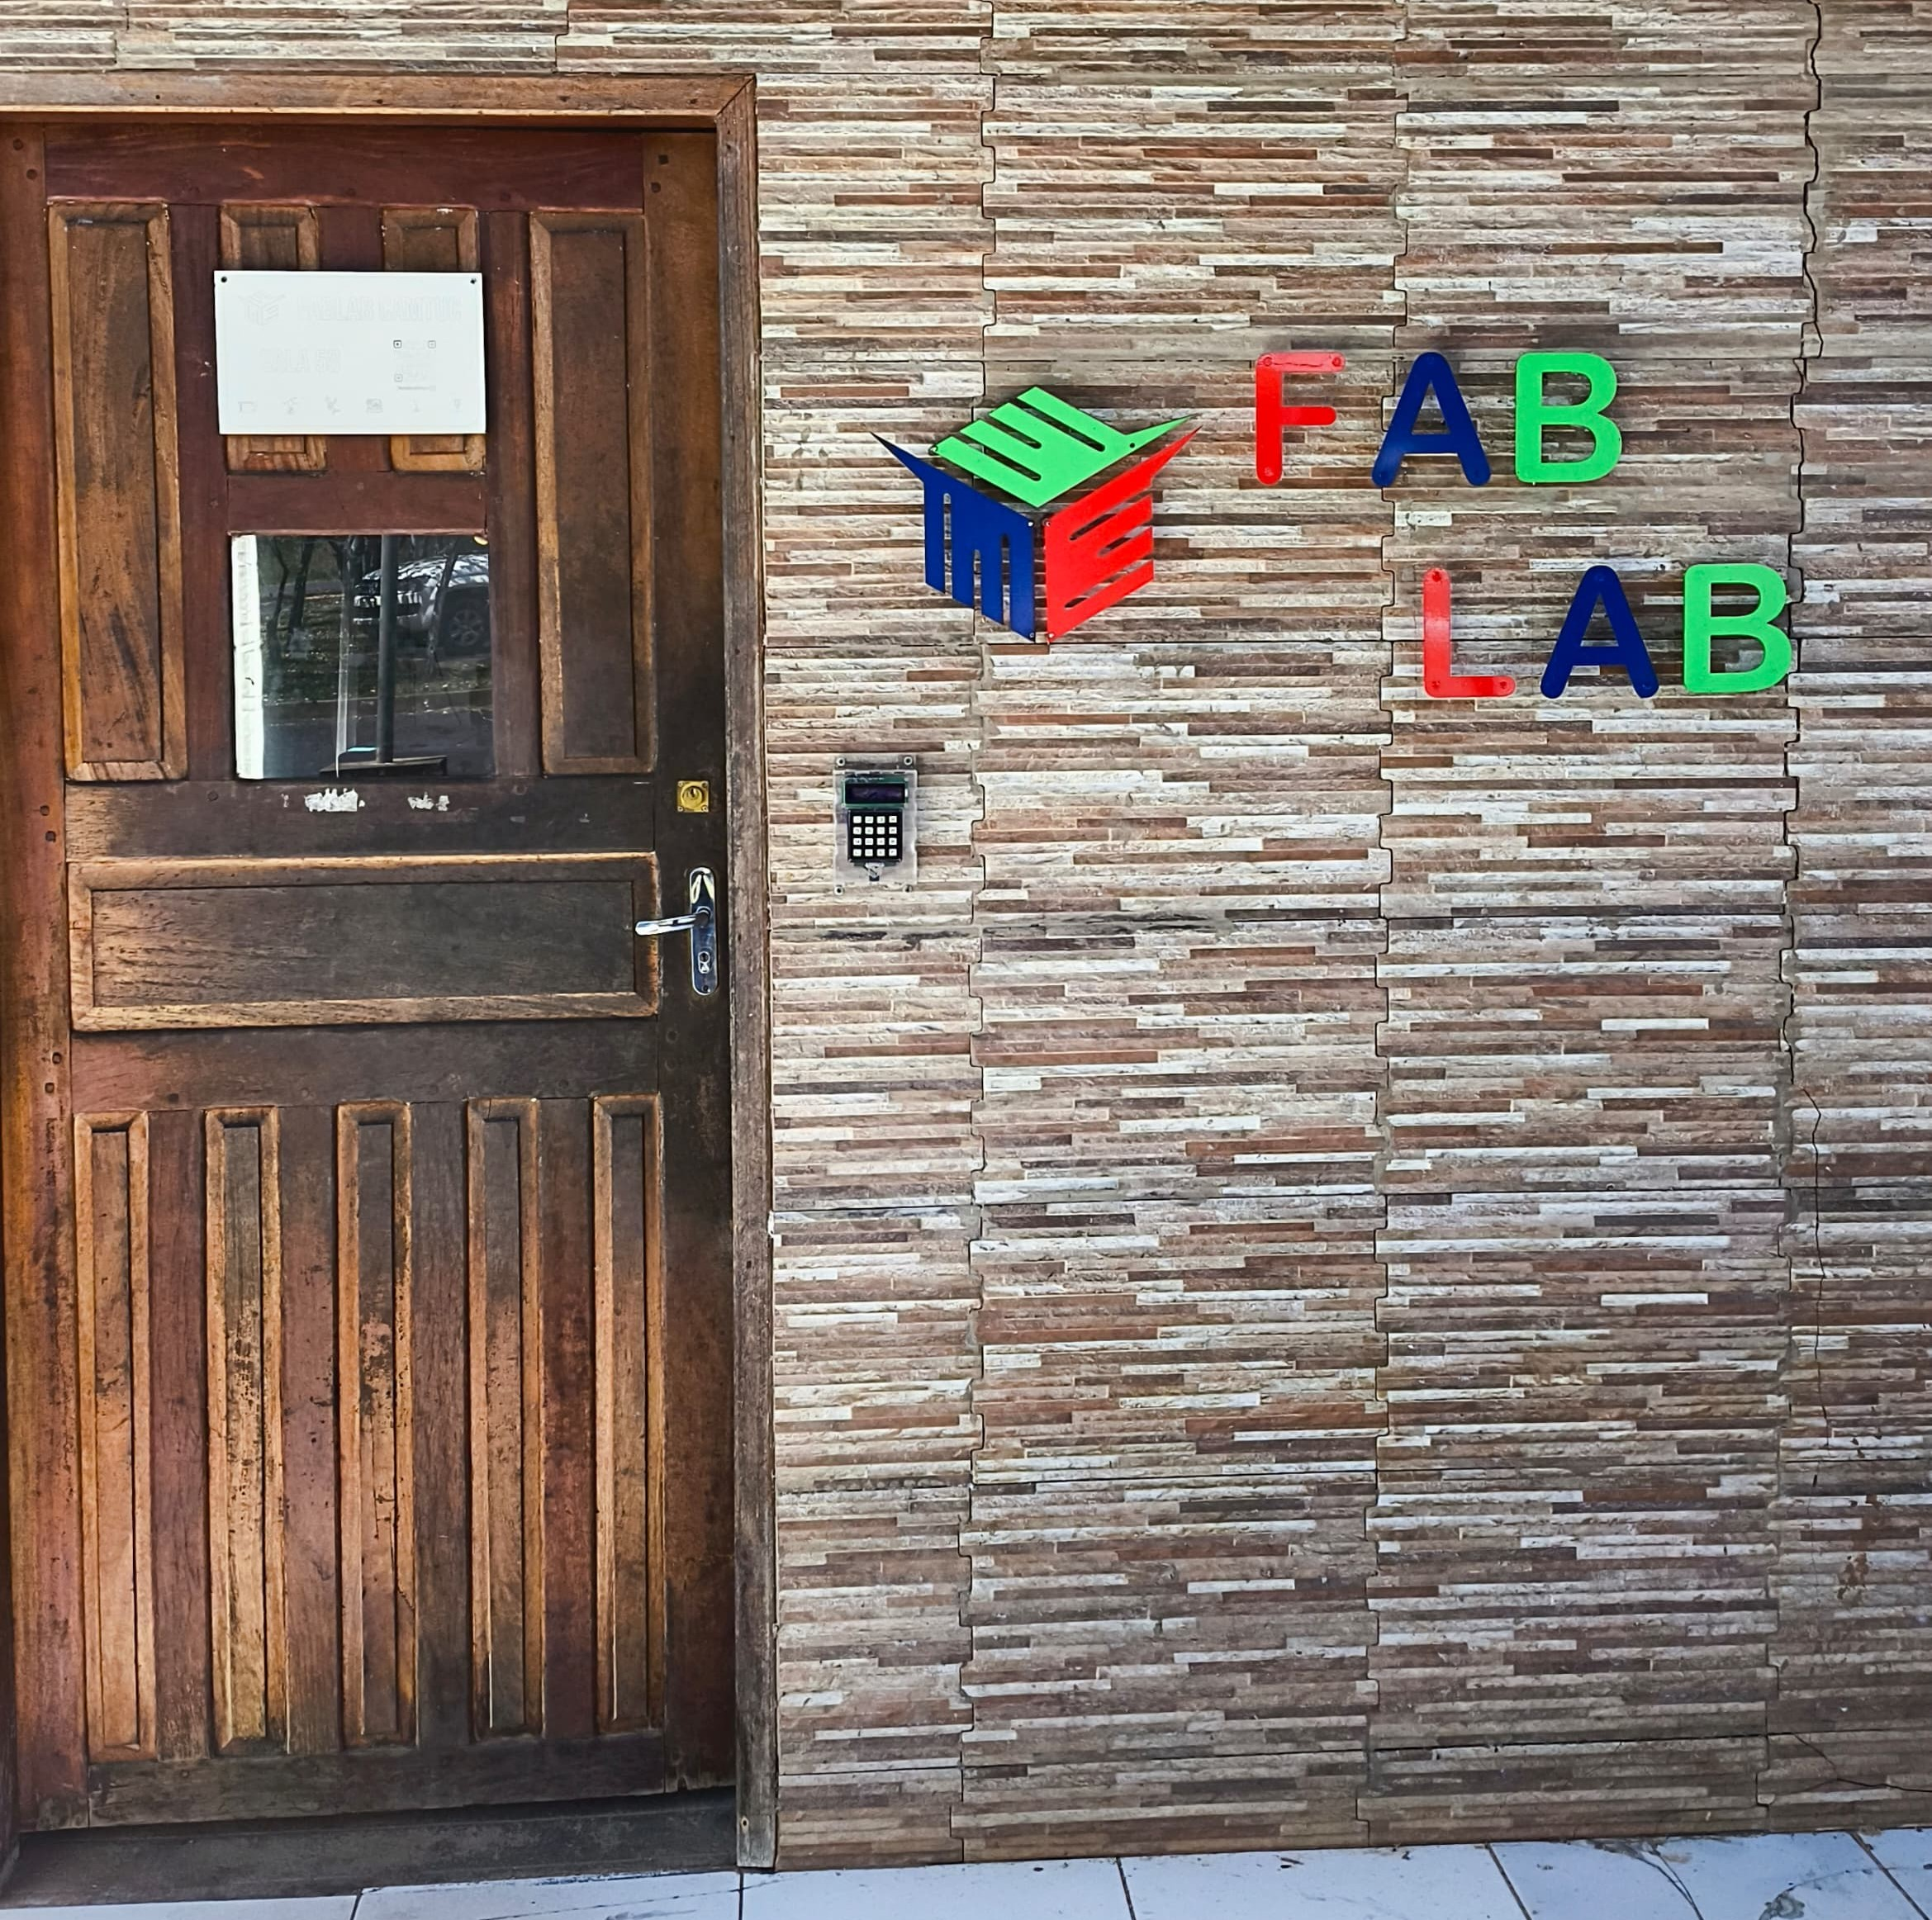
\includegraphics[width=0.5\textwidth,height=\textheight]{D:/Minha pasta/Estudos/UFPA/8º Semestre - 2024.2/Tópico Especiais em Eletrônica/Aluno/Ryan TEE/1.jpeg}

Fig 1: Entrada do FABLAB.

\chapter{PROCESSO DE IMPRESSÃO 3D}\label{processo-de-impressuxe3o-3d}

As primeiras máquinas que foram apresentadas foram as impressoras 3D, especificamente os modelos Creality Ender 3 disponíveis no laboratório. As impressoras 3D são máquinas CNC que fabricam objetos tridimensionais através do método aditivo, ou seja, constroem o objeto adicionando material camada por camada. Para isso, é necessário ter o arquivo digital do objeto desejado no formato G-code, que é a linguagem de máquina para várias CNCs, incluindo esses modelos de impressoras.

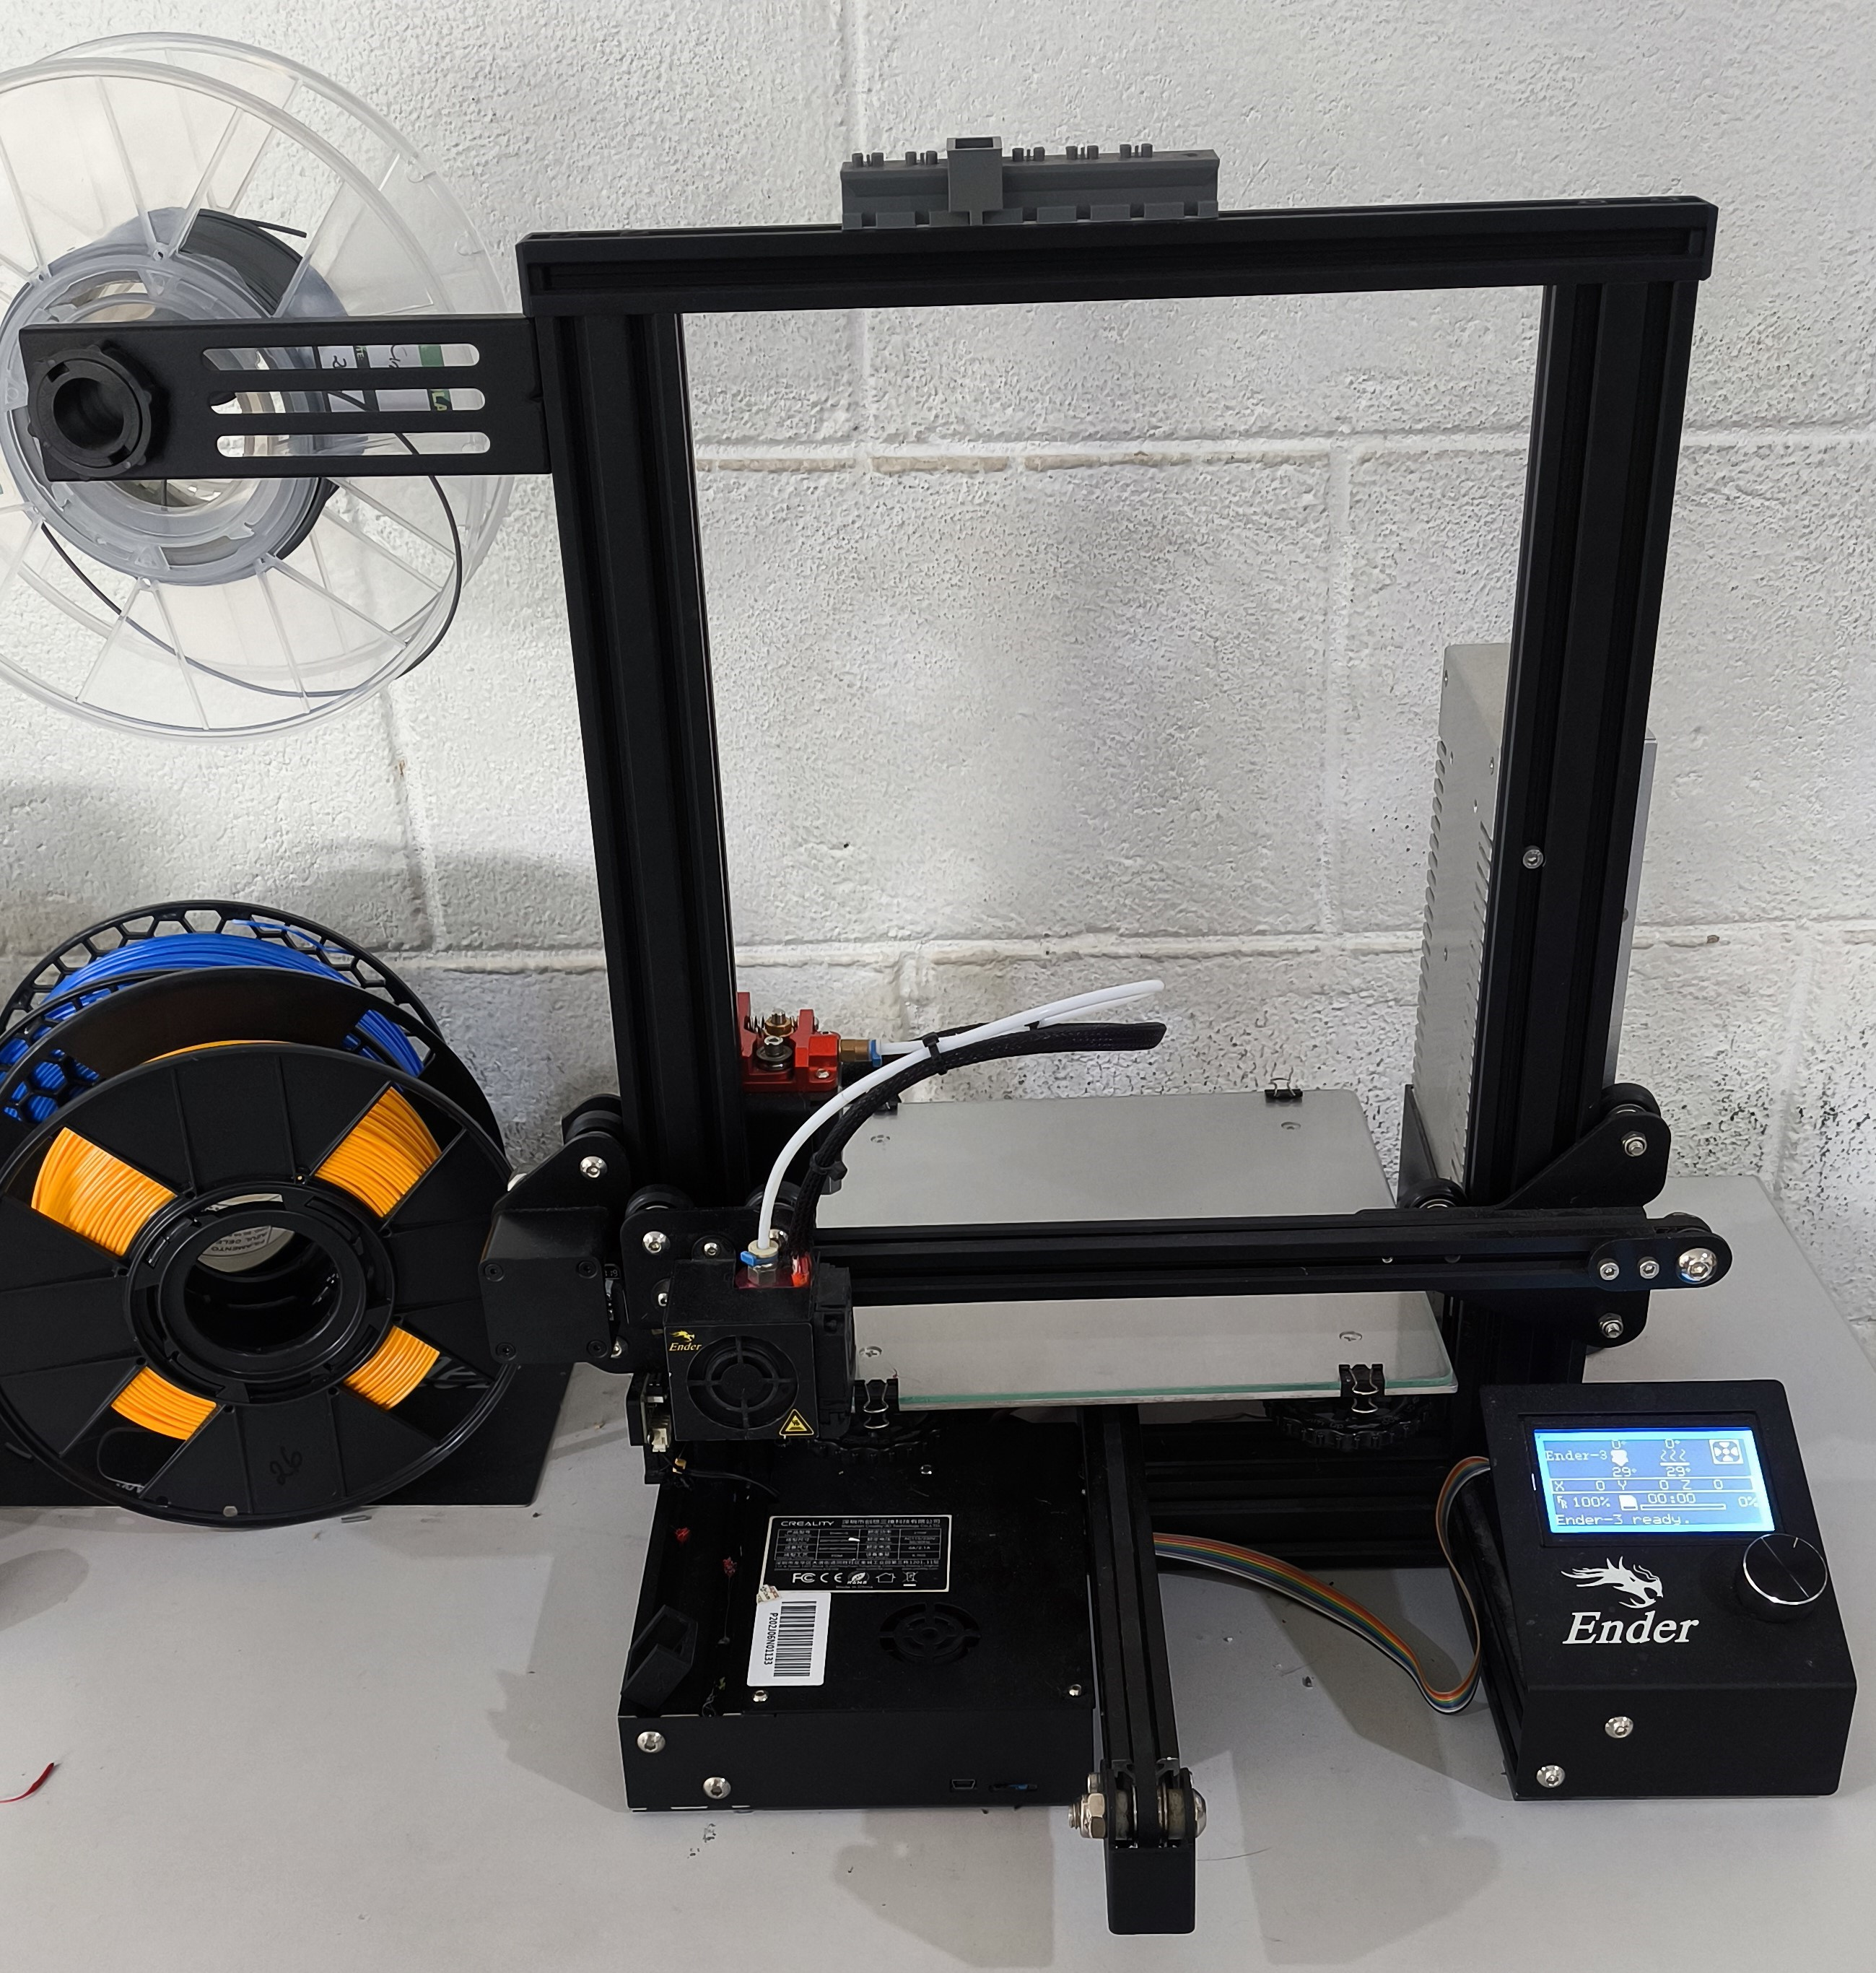
\includegraphics[width=0.4\textwidth,height=\textheight]{D:/Minha pasta/Estudos/UFPA/8º Semestre - 2024.2/Tópico Especiais em Eletrônica/Aluno/Ryan TEE/2.jpg}

Fig 2: Impressora Creality Ender 3.

\section{Filamentos}\label{filamentos}

Na fabricação de objetos através do processo de impressão 3D, são utilizados alguns tipos de plásticos chamados filamentos. Existem diversos tipos de filamentos, sendo os mais utilizados o PLA, ABS, PETG, TPU e PET.

PLA: O mais utilizado no FABLAB, é popular e fácil de trabalhar. Feito a partir de fontes renováveis, o PLA é um material de fácil impressão, ideal para impressoras abertas ou fechadas, com ou sem mesa aquecida, e não emite gases tóxicos.

ABS: Derivado do petróleo, é bastante utilizado na indústria. É resistente a altas temperaturas e impactos, com visual opaco. Recomenda-se usar em impressoras fechadas, pois pode liberar gases prejudiciais à saúde.

PETG: Um material mais resistente que o PLA, também não emite gases tóxicos e pode ser usado em impressoras abertas ou fechadas.

TPU: Ideal para objetos flexíveis e resistentes ao impacto, semelhante a borracha.

PET: Feito de garrafas PET, oferece o benefício da reciclagem e é economicamente viável. No FABLAB, há uma extrusora de garrafa PET e uma impressora separada exclusivamente para este filamento, que é bastante resistente a impactos, umidade e temperatura.

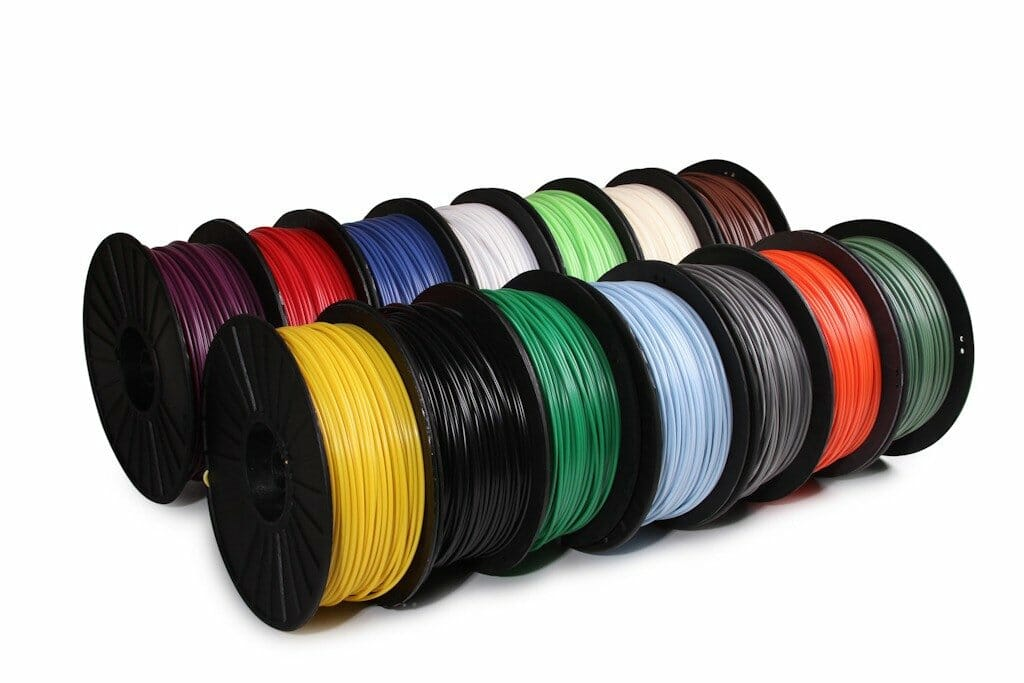
\includegraphics[width=0.45\textwidth,height=\textheight]{D:/Minha pasta/Estudos/UFPA/8º Semestre - 2024.2/Tópico Especiais em Eletrônica/Aluno/Ryan TEE/3.jpeg}

Fig 3: Exemplos de filamentos.

\section{funcionamento da Impressora 3D}\label{funcionamento-da-impressora-3d}

Os modelos de impressoras 3D no FABLAB funcionam com base em quatro motores de passo: três responsáveis pelos eixos X, Y e Z, e um para puxar o filamento.

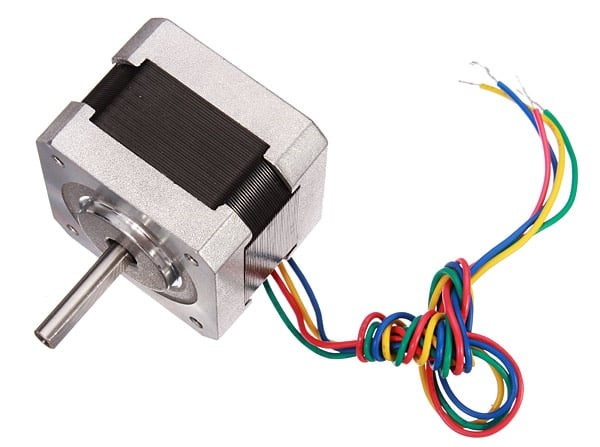
\includegraphics[width=0.4\textwidth,height=\textheight]{D:/Minha pasta/Estudos/UFPA/8º Semestre - 2024.2/Tópico Especiais em Eletrônica/Aluno/Ryan TEE/4.jpg}

Fig 4: Motor de passo.

Eixo X: Movimenta da esquerda para a direita através de um sistema de correia, onde está acoplada a extrusora, que contém o hotend, sensores de temperatura, cooler de refrigeração e o bico da impressora. O hotend aquece o filamento à temperatura ideal, tornando-o maleável para a modelagem do objeto.

O diâmetro do bico influencia na qualidade e no tempo da impressão, com os principais bicos usados no laboratório tendo diâmetros de 0,2 mm, 0,4 mm, 0,5 mm e 0,8 mm.

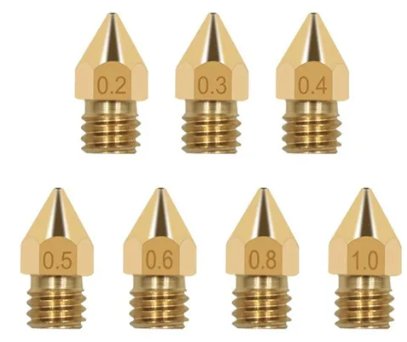
\includegraphics[width=0.4\textwidth,height=\textheight]{D:/Minha pasta/Estudos/UFPA/8º Semestre - 2024.2/Tópico Especiais em Eletrônica/Aluno/Ryan TEE/5.png}

Fig 5: Bicos para impressoras 3D.

Eixo Y: Movimenta a mesa da impressora, que na mesa contém uma resistência para aquecimento, melhorando a fixação do objeto durante a impressão.

Eixo Z: O Motor do eixo Z é acoplado a um fuso, que é responsável pelo movimento para cima e para baixo da impressora, mas durante o processo de impressão, o eixo Z só se movimenta apenas para cima, evitando que bata na peça, começando da origem do eixo e vai subindo camada pro camada.

Para maquina ter a referência de posicionamento, cuja é suma importância, é utilizado sensores de fim de curso mecânicos, de modo que eles representam as origens de cada eixo. A interface desse tipo de impressora é feita através de um botão rotativo e um display, de modo que controlar a máquina.

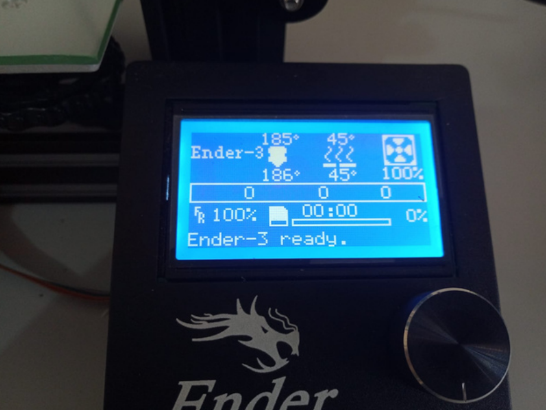
\includegraphics[width=0.5\textwidth,height=\textheight]{D:/Minha pasta/Estudos/UFPA/8º Semestre - 2024.2/Tópico Especiais em Eletrônica/Aluno/Ryan TEE/6.png}

Fig 6: Painel da impressora Creality Ender 3.

O arquivo digital pode ser passado de duas maneiras, sendo uma através de cartão de memória e posteriormente o processo é iniciado através da interface da impressora ou controlada diretamente pelo computador via cabo.

\section{Modelagem 3D}\label{modelagem-3d}

A modelagem 3D é basicamente transformar o desenho de um objeto em uma representação digital tridimensional. No FABLAB, os softwares CAD (Computer Aided Design) mais usados para modelagens 3D são o Fusion 360 e o SolidWorks, que são bem parecidos na forma de usar. Geralmente, a modelagem começa com o desenvolvimento do desenho em 2D e depois se faz a extrusão do objeto para transformá-lo em 3D. Em seguida, são feitos os ajustes necessários na peça.

A dificuldade desse processo depende diretamente da complexidade da peça a ser desenvolvida. No geral, esses dois softwares são bem intuitivos e têm uma capacidade de desenvolvimento muito grande, permitindo criar desde peças simples até as mais complexas.


\includegraphics[width=0.6\textwidth,height=\textheight]{D:/Minha pasta/Estudos/UFPA/8º Semestre - 2024.2/Tópico Especiais em Eletrônica/Aluno/Ryan TEE/7.png}

Fig 7: Softwares para modelagem 3D.

\section{Fatiamento}\label{fatiamento}

Depois de modelar um objeto em 3D, para imprimi-lo é necessário fazer o fatiamento. Isso significa pegar a geometria do modelo e transformá-la em instruções que a máquina CNC entende, ou seja, o arquivo G-code. O primeiro passo é exportar o arquivo do software de modelagem 3D no formato STL (Standard Tessellation Language). Em seguida, utilizamos outro software para fazer o
fatiamento, no caso o UltiMaker Cura. Para usar o Cura corretamente, é importante adicionar o modelo da impressora que será utilizado, pois isso garante que os parâmetros, como área de trabalho, temperatura e velocidade máxima, estejam corretos.

Depois, configuramos o diâmetro do bico da impressora e o tipo de filamento a ser usado. A seguir, ajustamos os parâmetros da impressão. Primeiro, definimos a qualidade de resolução da peça, que basicamente é a altura de cada camada; quanto mais fina a camada, melhor a qualidade, mas o tempo de impressão será maior. Também ajustamos a espessura das paredes, da base e do topo da peça.

O próximo passo é escolher o tipo de preenchimento e a densidade do material, que é dada em porcentagem: 0\% significa uma peça oca e 100\% uma peça maciça. Depois, ajustamos a temperatura do bico e da mesa da impressora, que varia conforme o tipo de filamento, e a velocidade da impressão. Um parâmetro importante é a existência de suporte, que depende da forma do objeto e de como ele está posicionado na mesa; o suporte é necessário em peça onde o percurso do bico iria depositar material no ar.

Após configurar tudo, basta apertar o botão para fazer o fatiamento, que gera o arquivo G-code. Esse arquivo pode ser passado para a impressora via cartão de memória ou diretamente pelo computador.

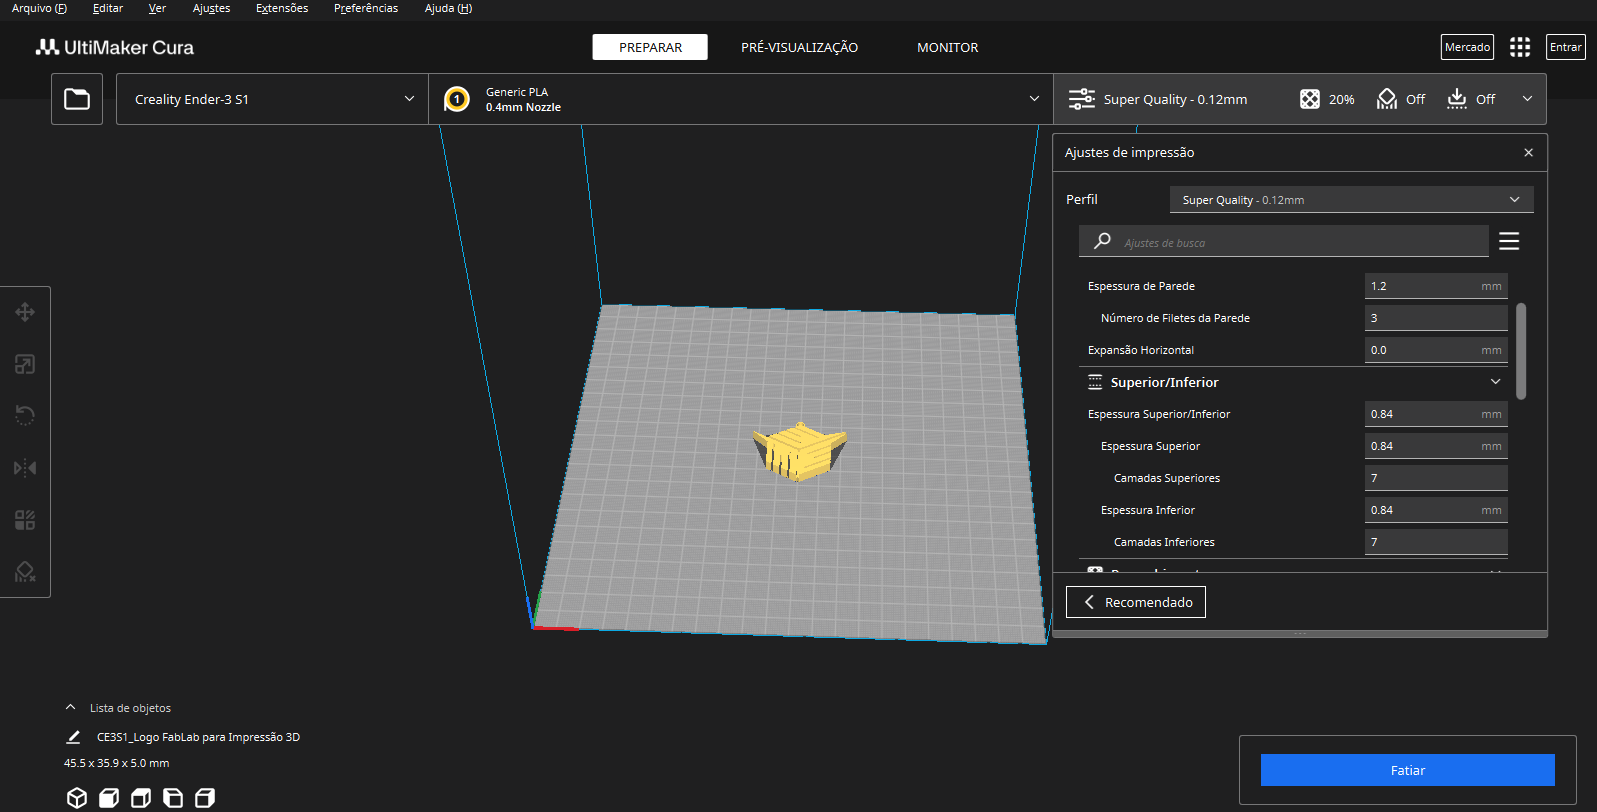
\includegraphics[width=0.6\textwidth,height=\textheight]{D:/Minha pasta/Estudos/UFPA/8º Semestre - 2024.2/Tópico Especiais em Eletrônica/Aluno/Ryan TEE/8.png}

Fig 8: Exemplo de fatiamento.

Como membro do FABLAB e monitor da disciplina, ajudei os demais alunos a fazerem suas impressões, utilizando as máquinas corretamente e fazendo o fatiamento adequado para cada impressão. Para agilizar o processo, foi recomendado eles utilizarem o site Thingiverse, onde há muitos arquivos prontos de objetos 3D disponíveis para download no formato STL. Também é essencial nivelar a mesa da impressora para garantir uma boa qualidade na impressão, usando uma folha de papel para ajustar a distância entre a mesa e o bico quando o eixo Z está na origem. O nivelamento é feito através de quatro parafusos localizados nos cantos da mesa.

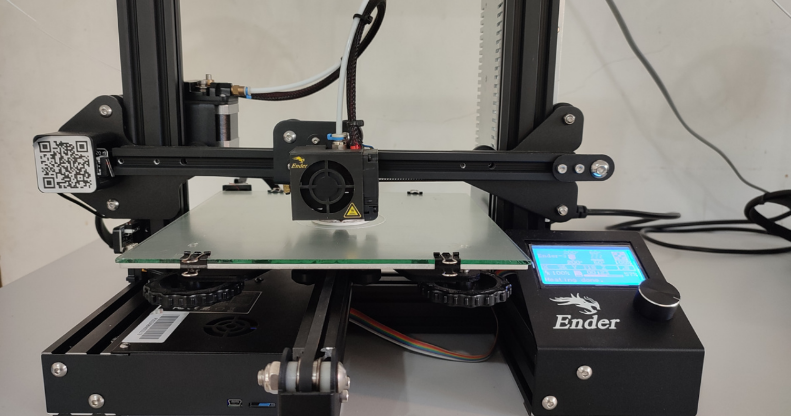
\includegraphics[width=0.6\textwidth,height=\textheight]{D:/Minha pasta/Estudos/UFPA/8º Semestre - 2024.2/Tópico Especiais em Eletrônica/Aluno/Ryan TEE/9.png}

Fig 9: Mesa da impressora 3D.

\chapter{CORTE E GRAVAÇÃO A LASER}\label{corte-e-gravauxe7uxe3o-a-laser}

A próxima máquina apresentada para os alunos foi a Router Laser CNC VS6040, com potência de 60 W. Ela realiza corte e gravação em vários tipos de materiais, possuindo uma ampla área de utilização. No FABLAB, os materiais mais utilizados são o acrílico, papelão, MDF e outros tipos de madeira.

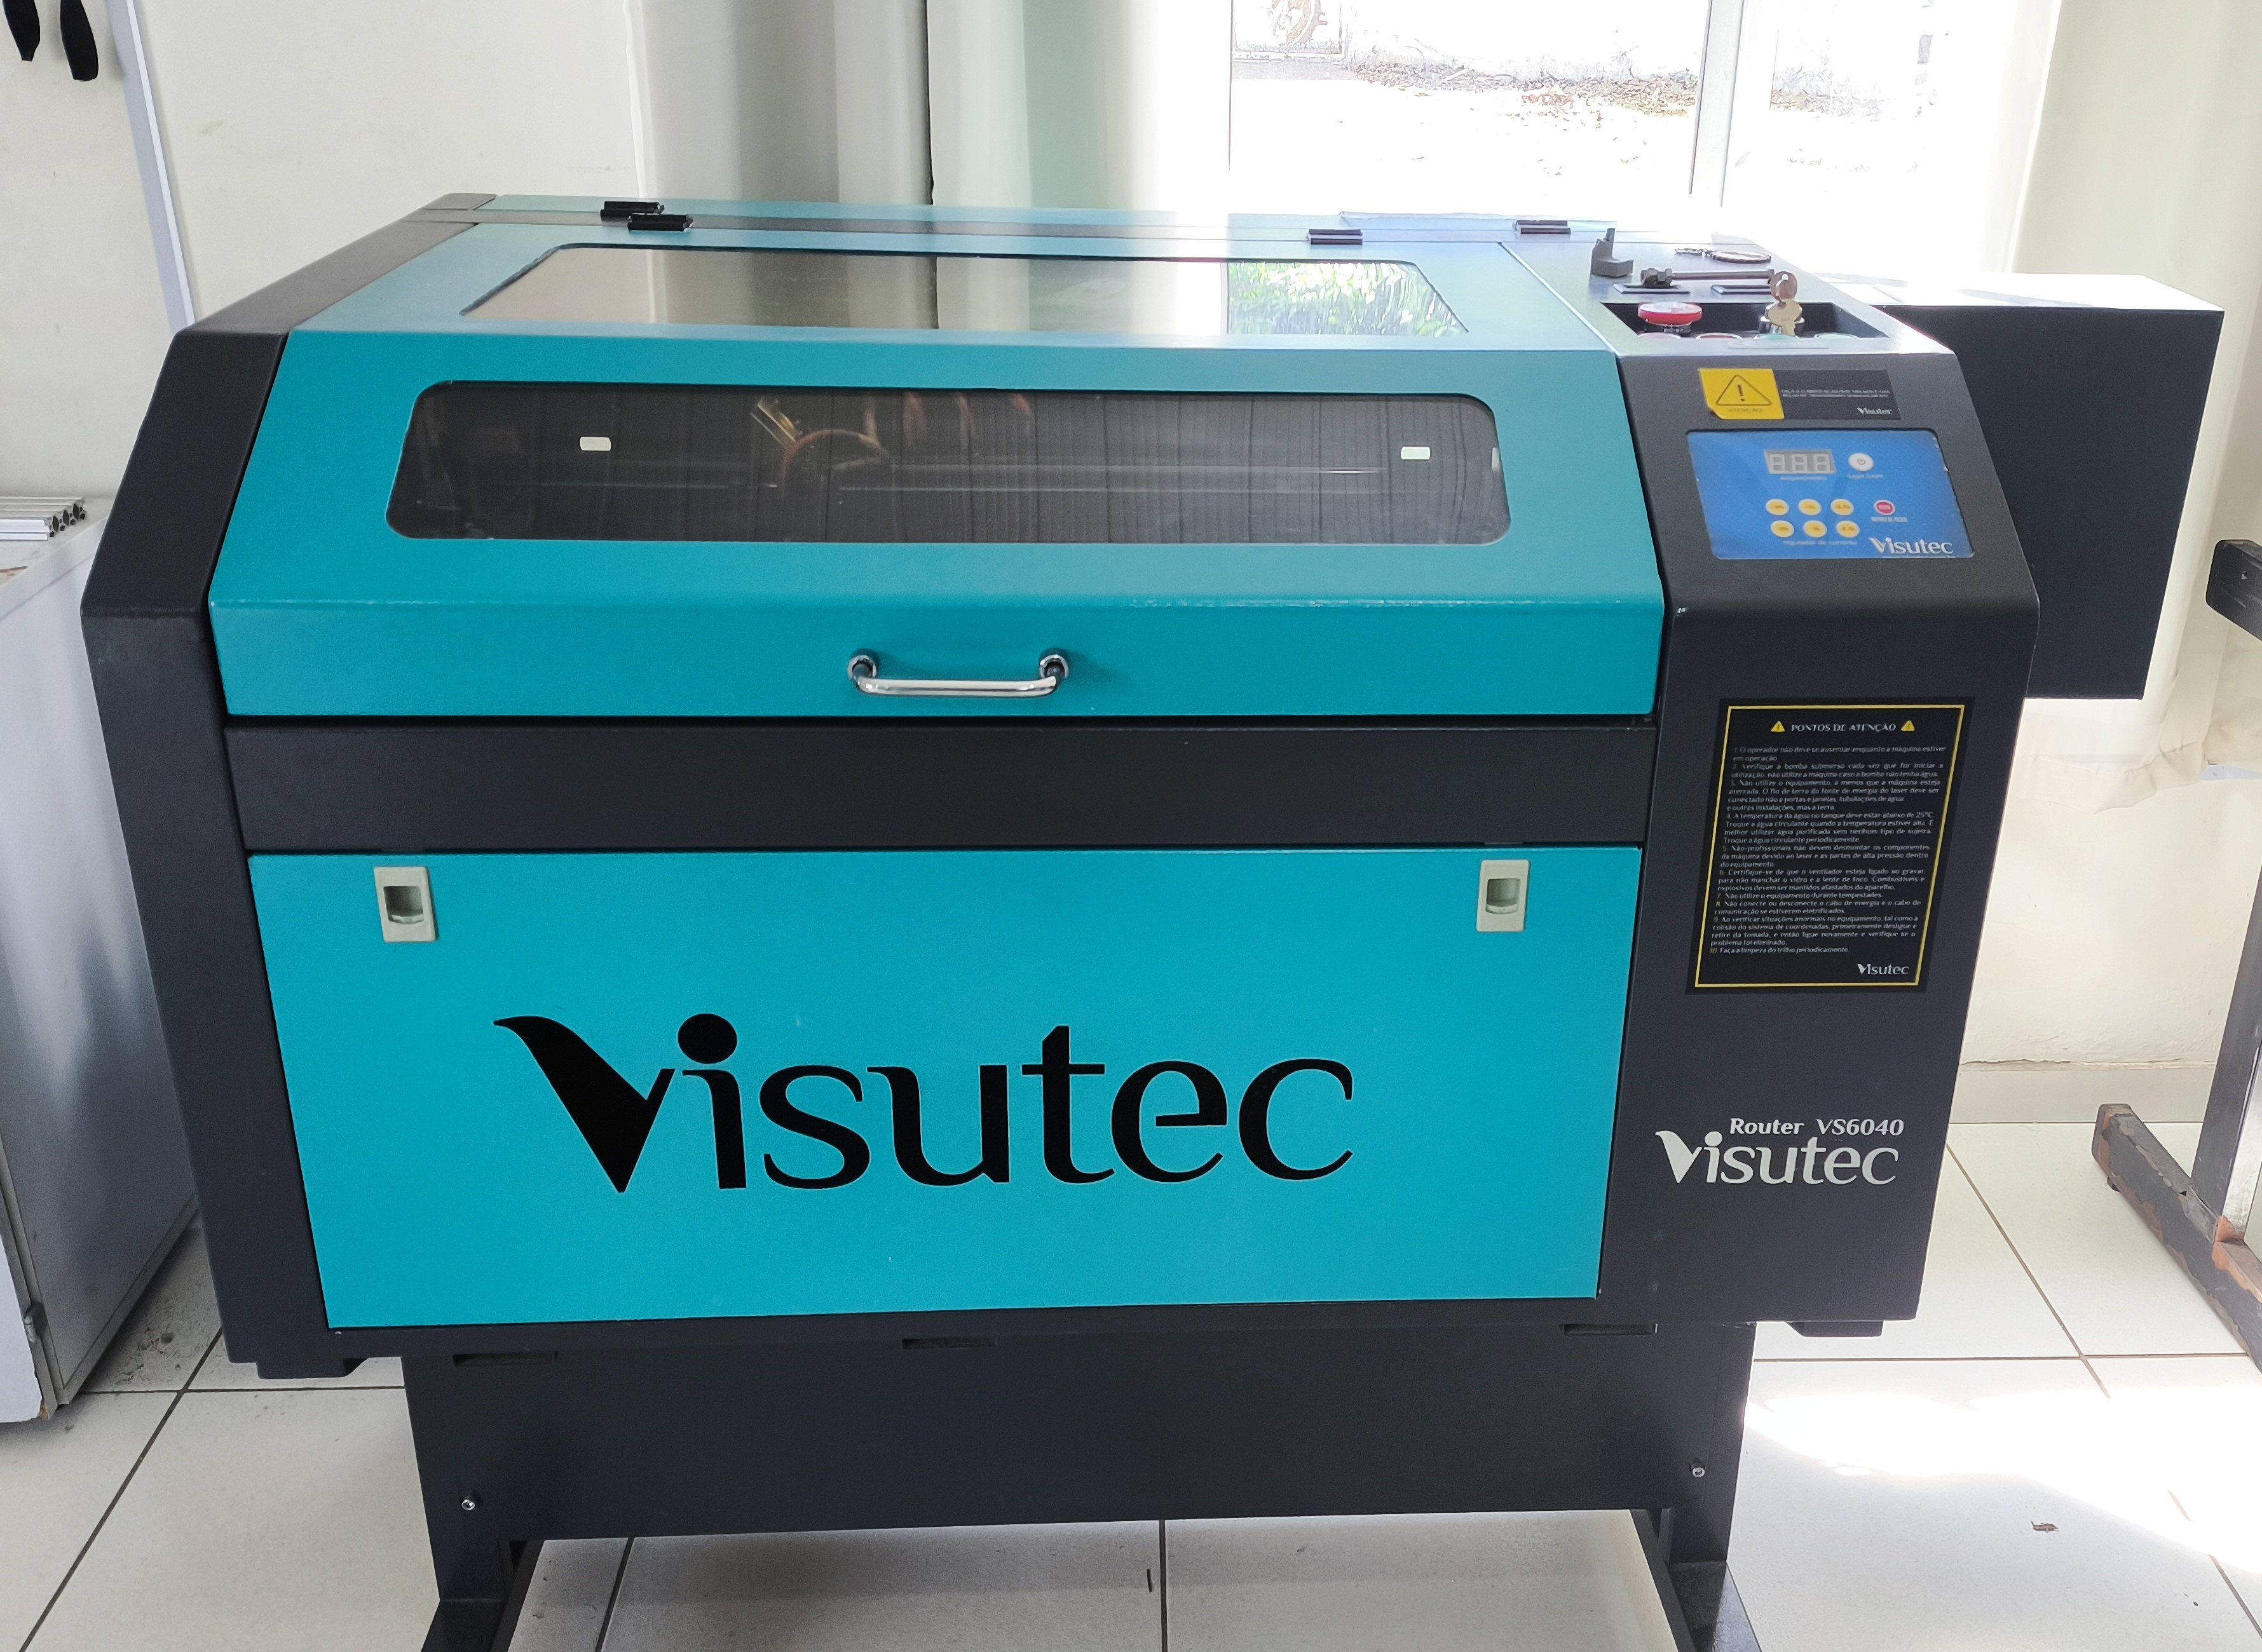
\includegraphics[width=0.6\textwidth,height=\textheight]{D:/Minha pasta/Estudos/UFPA/8º Semestre - 2024.2/Tópico Especiais em Eletrônica/Aluno/Ryan TEE/10.jpg}

Fig 10: Máquina Router Laser.

\section{Desenho 2D}\label{desenho-2d}

Para realizar cortes e gravações na router laser, é necessário ter um desenho em 2D, vetorizado no formato SVG (Scalable Vector Graphics). Existem vários softwares capazes de criar desenhos vetorizados, mas os principais utilizados no FABLAB são o Inkscape e o CorelDRAW. A comunicação entre o computador e a máquina é feita pelo software K40 Whisperer, que é bem simples de usar. Ele é baseado em três operações, associadas às cores da paleta RGB: preto para gravação (raster engrave), vermelho para corte (vector cut) e azul para gravação em linhas (vector engrave). No software de desenho, é preciso especificar essas cores para obter o produto desejado, onde a cor preta (gravação) é preenchida e as cores vermelha e azul (corte e gravação em linhas) são contornos.

\section{Funcionamento do laser}\label{funcionamento-do-laser}

Essa máquina também se movimenta através de motores de passo acoplados a um sistema de correia. São dois motores, um para o eixo X e outro para o eixo Y, fazendo com que seja considerada uma máquina em duas dimensões. Há também um terceiro motor, responsável por ajustar a altura do material em relação ao bico do laser. Esse ajuste é feito através de um gabarito, que garante que a distância do bico ao material permita que o feixe do laser seja o mais fino possível, proporcionando um melhor acabamento.

O laser é gerado na parte de trás da máquina, através de um tubo de CO2. O feixe do laser é direcionado por meio de três espelhos até chegar ao bico do laser, também chamado de canhão, que está acoplado ao eixo X. Dentro do canhão há uma lente que foca os feixes em uma área menor.

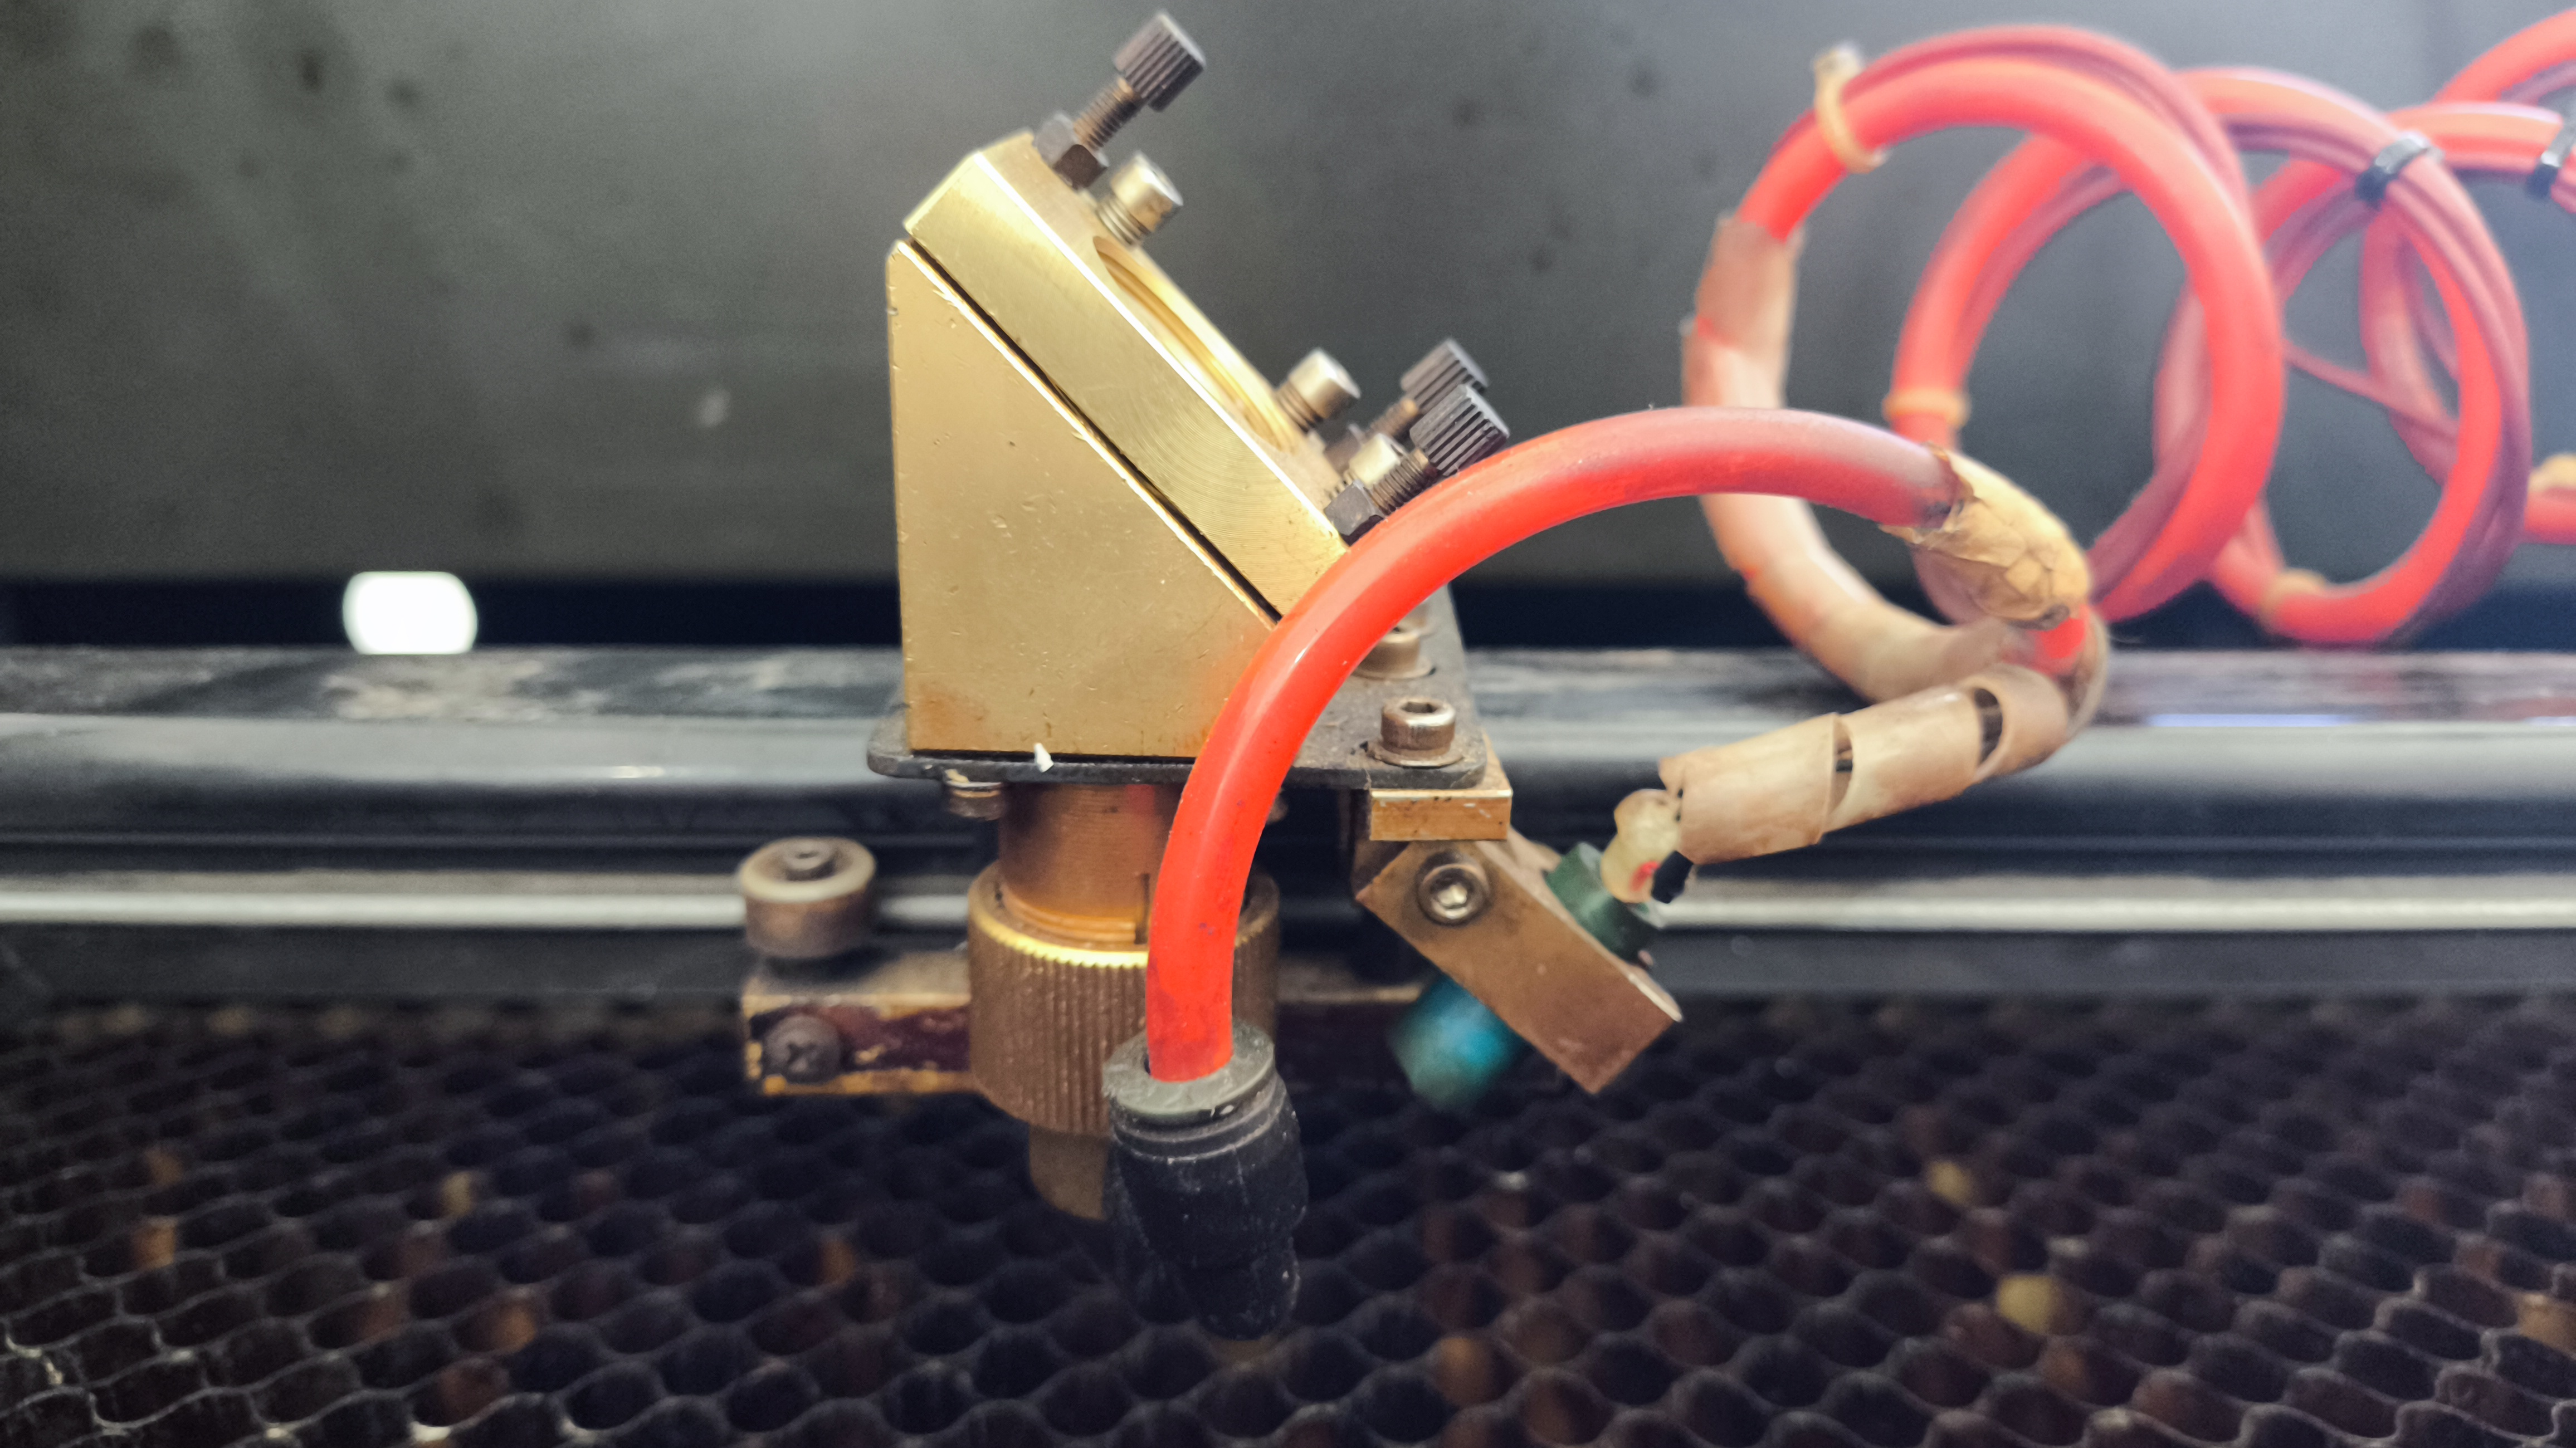
\includegraphics[width=0.6\textwidth,height=\textheight]{D:/Minha pasta/Estudos/UFPA/8º Semestre - 2024.2/Tópico Especiais em Eletrônica/Aluno/Ryan TEE/11.jpg}

Fig 11: Canhão do laser.

O tubo do laser é resfriado por um sistema de bombeamento de água, e é importante monitorar a temperatura do laser e da água de resfriamento. Durante a operação, o laser emite bastante fumaça. Por isso, há um exaustor na parte inferior da máquina, conectado a uma tubulação que expulsa a fumaça para fora do laboratório.

A máquina possui um painel relativamente simples, com uma chave para ligar e desligar, um botão de emergência que desliga completamente, dois botões para descer ou subir a mesa, um botão para ligar a lâmpada interna e outro para ligar ou desligar o exaustor. Há também um controle de potência do laser, ajustável conforme o material e a ação desejada, seja corte ou gravação. A velocidade de cada ação é controlada pelo software K40 Whisperer.

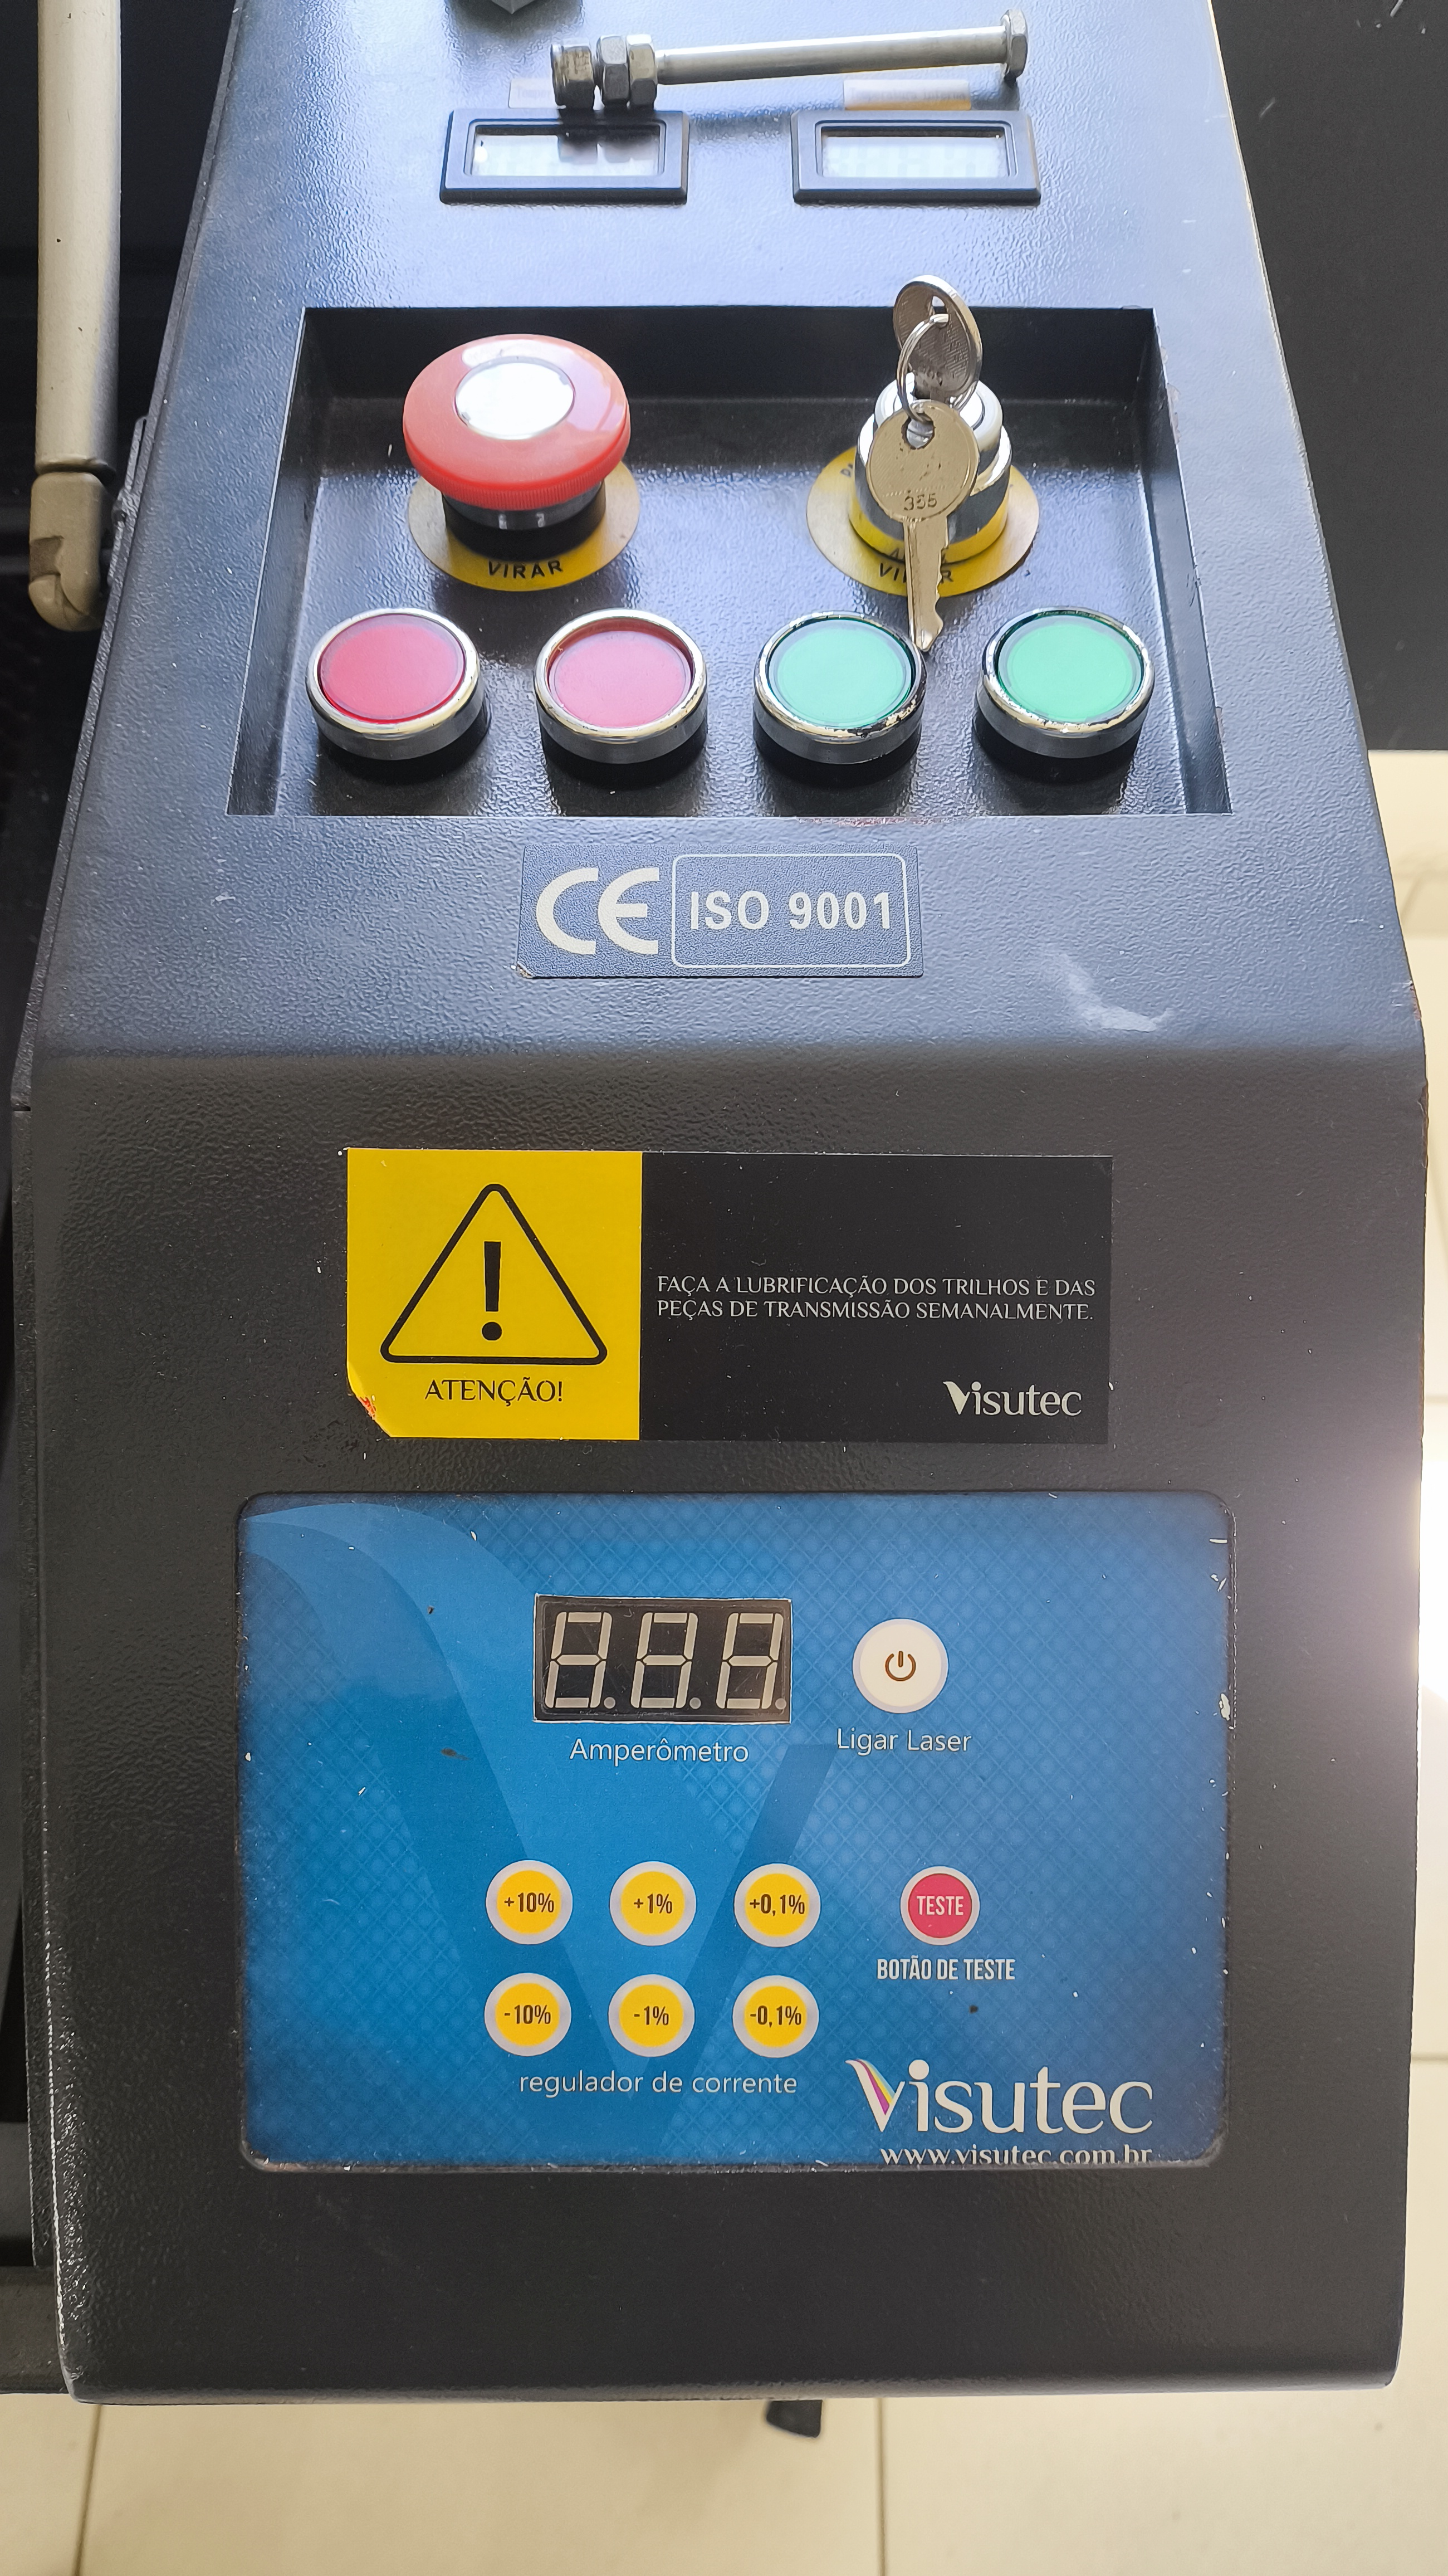
\includegraphics[width=0.4\textwidth,height=\textheight]{D:/Minha pasta/Estudos/UFPA/8º Semestre - 2024.2/Tópico Especiais em Eletrônica/Aluno/Ryan TEE/12.jpg}

Fig 12: Painel do laser.

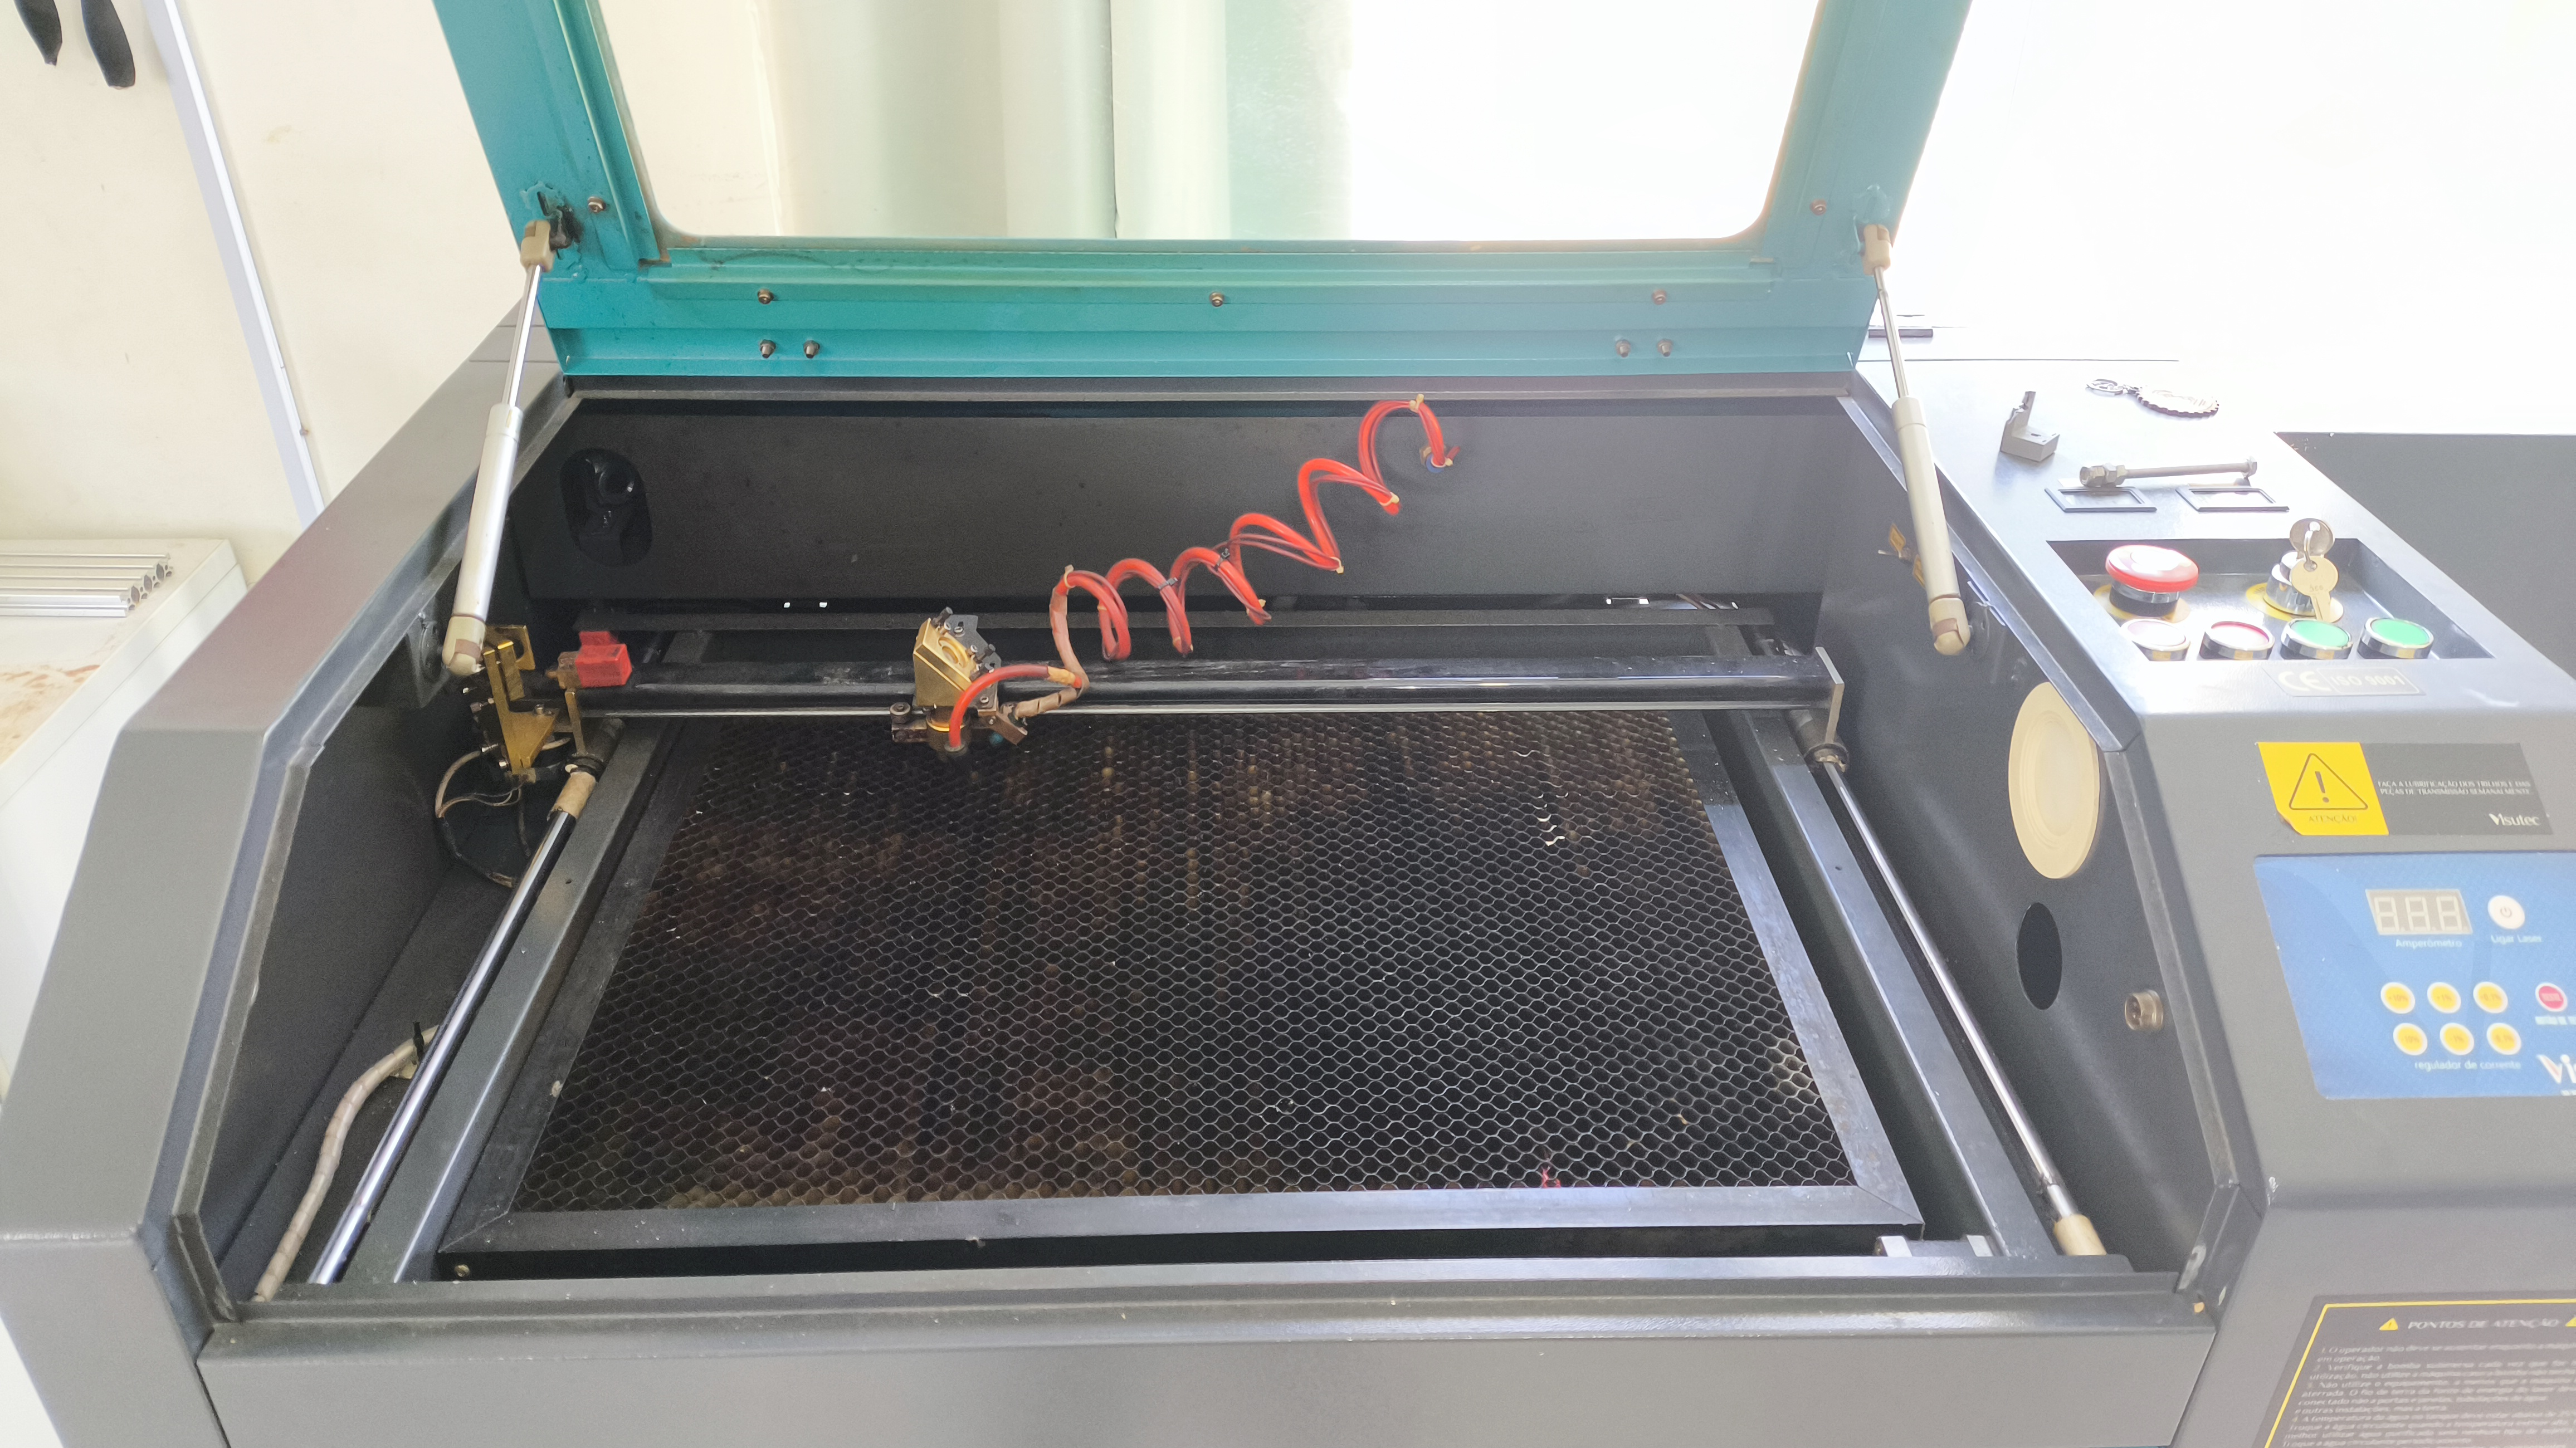
\includegraphics[width=0.6\textwidth,height=\textheight]{D:/Minha pasta/Estudos/UFPA/8º Semestre - 2024.2/Tópico Especiais em Eletrônica/Aluno/Ryan TEE/13.jpg}

Fig 13: Mesa do laser.

Depois da explicação teórica pelo professor, ajudei os alunos a projetarem e fabricarem um exemplo prático para usar o laser. A maioria optou por criar caixas, utilizando o site MakerCase, que facilita o design de vários tipos de caixas de maneira simples e rápida. Posteriormente, os alunos fizeram personalizações usando o Inkscape. Instrui-os sobre o uso correto e seguro do laser, já que a máquina tem um grau de perigosidade que pode causar acidentes. No final, foi uma atividade produtiva, e a maioria compreendeu bem todo o processo.

\chapter{FRESADORA (BIG FRESA)}\label{fresadora-big-fresa}

Outra máquina que foi apresentada é a fresadora, conhecida por Big Fresa. Ela é uma CNC que realiza o processo de usinagem e é capaz de fabricar peças tridimensionais de vários tipos. No FABLAB, o principal material usado na Big Fresa é a madeira. O processo é subtrativo, o que significa que você começa com um bloco de material e a máquina vai removendo partes até chegar na peça desejada. Ela é a uma máquina com grande área de trabalho, o que permite criar peças grandes e complexas. Como toda CNC, a Big Fresa oferece alta precisão, gerando peças de excelente qualidade, especialmente quando a máquina está bem calibrada.

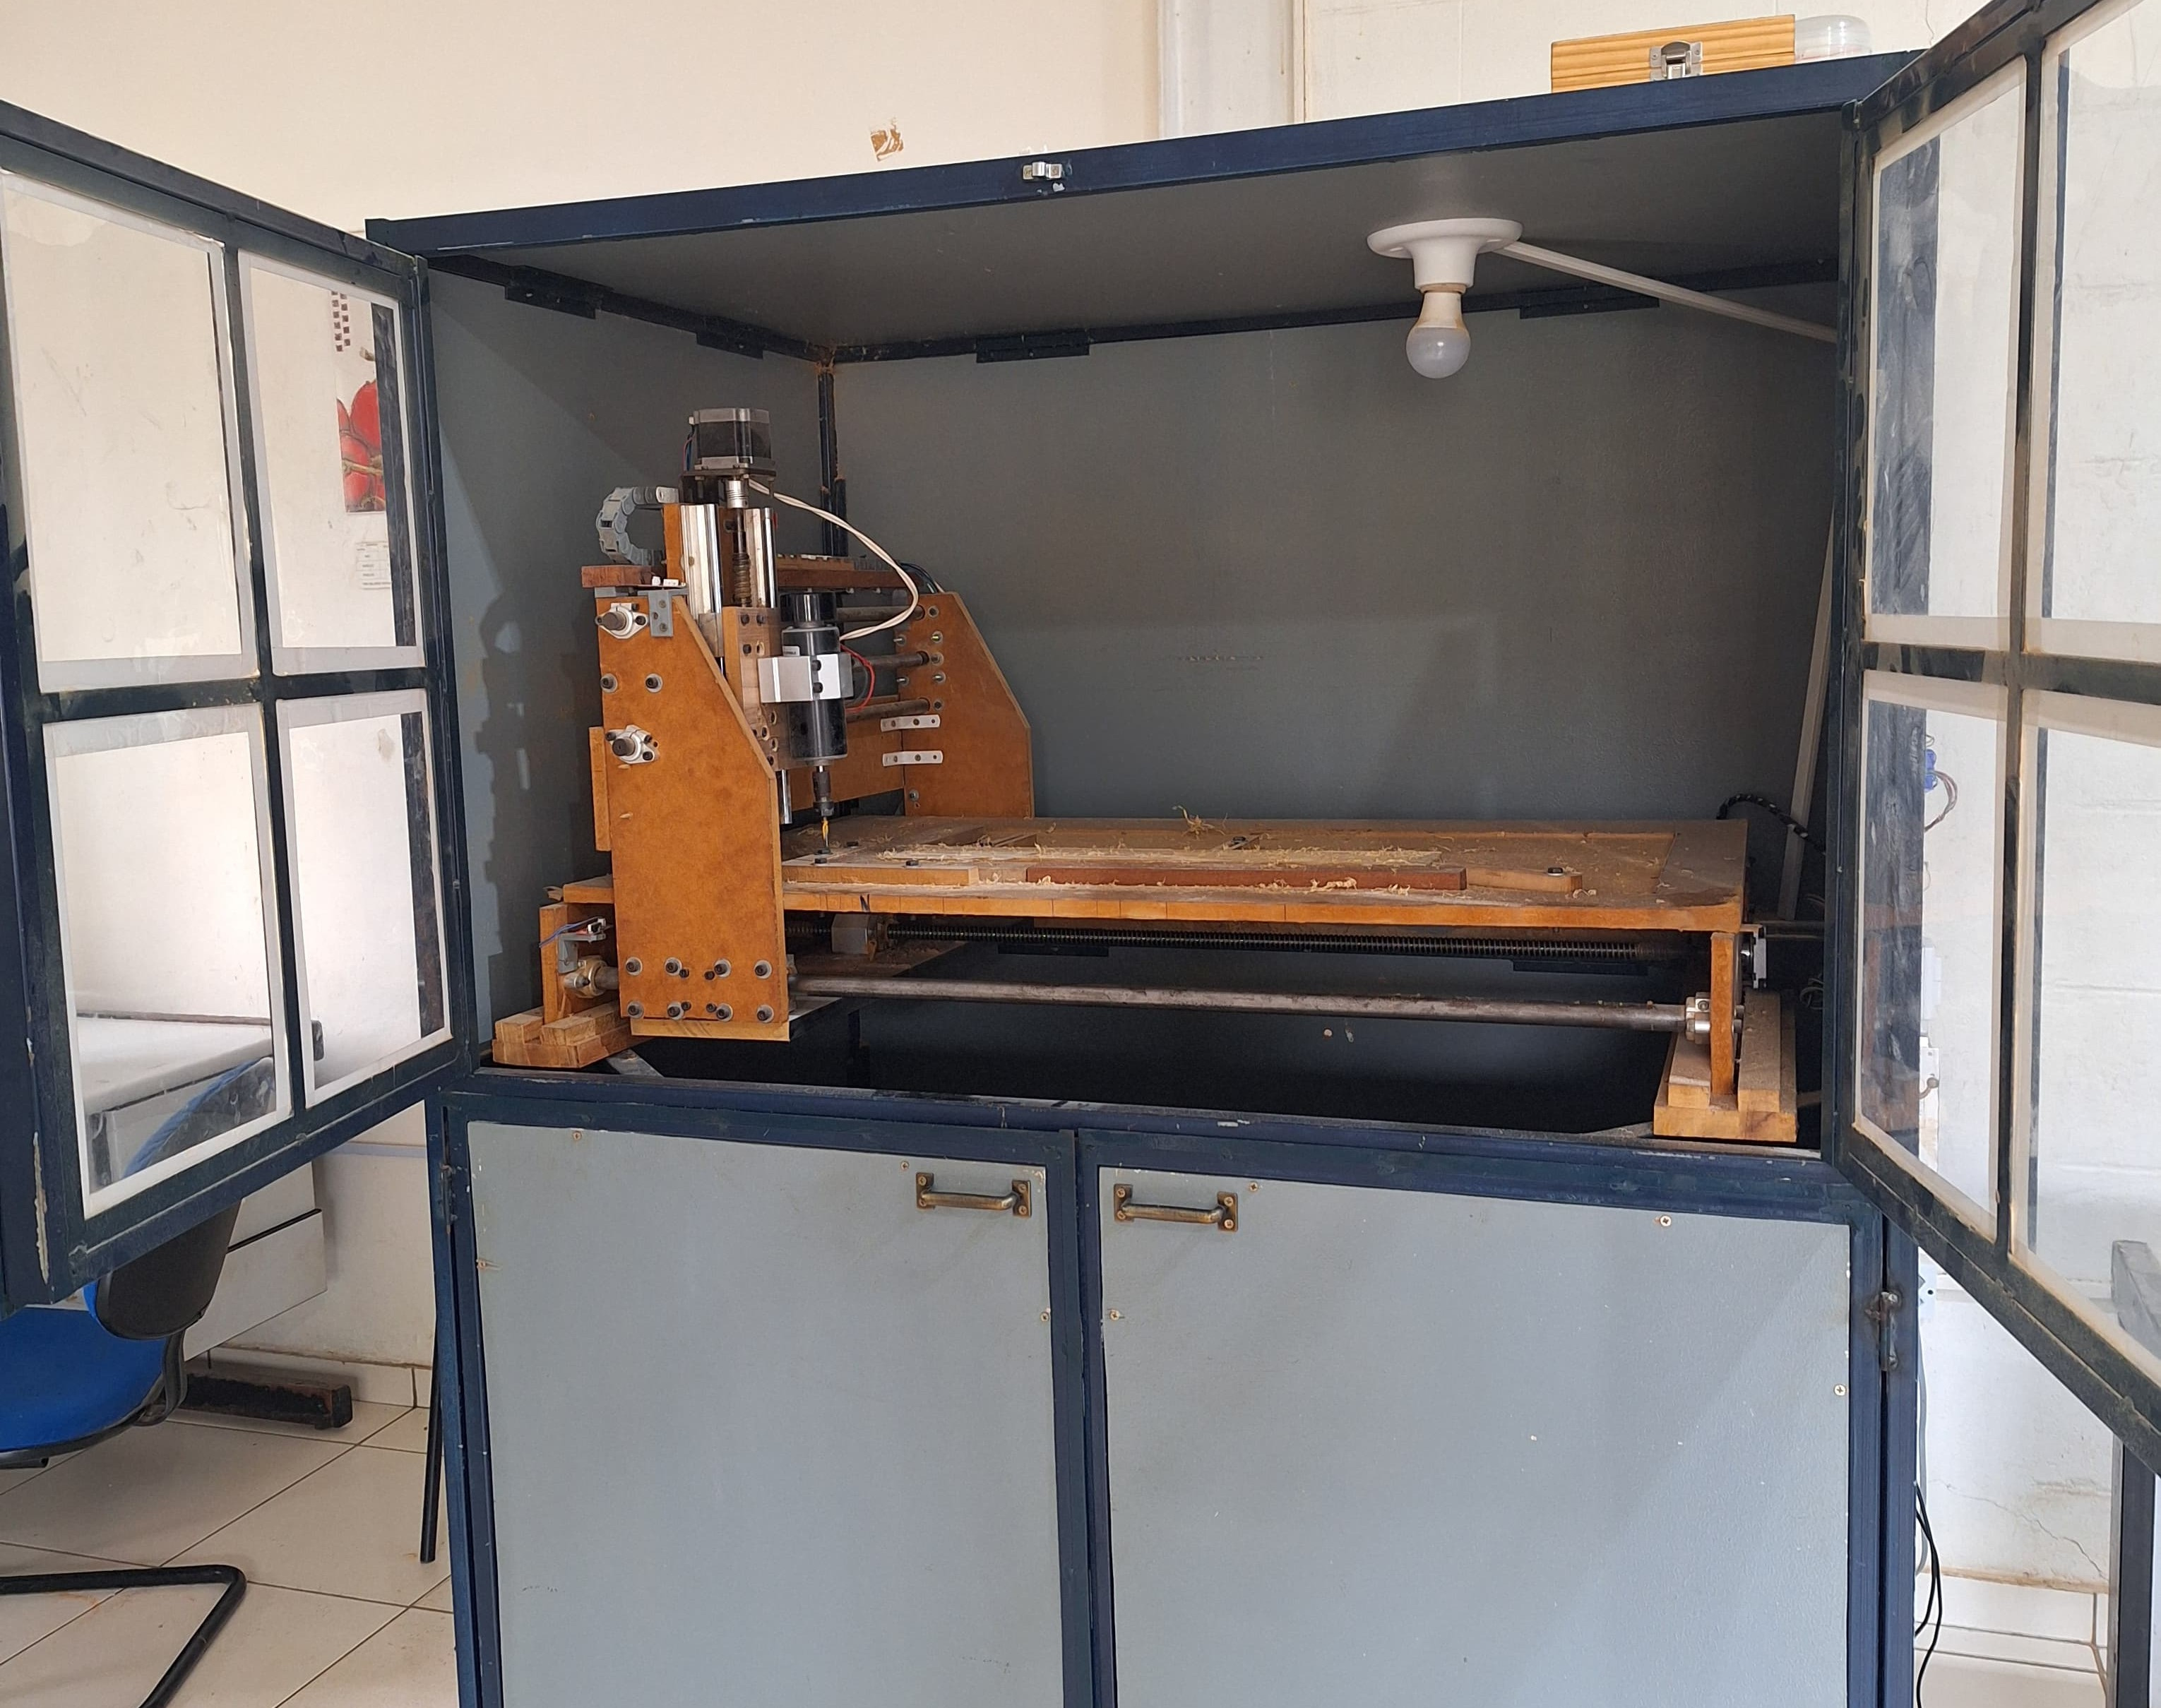
\includegraphics[width=0.5\textwidth,height=\textheight]{D:/Minha pasta/Estudos/UFPA/8º Semestre - 2024.2/Tópico Especiais em Eletrônica/Aluno/Ryan TEE/14.jpeg}

Fig 14: Big Fresa.

\section{Funcionamento da Big Fresa}\label{funcionamento-da-big-fresa}

A Big Fresa usa motores de passo para seus movimentos, com três motores responsáveis pelos eixos X, Y e Z. A transmissão é feita por fusos em todos os eixos. A usinagem é realizada pelo spindle, que é um motor DC específico para fresadoras, com uma velocidade de rotação de até 12.000 RPM.

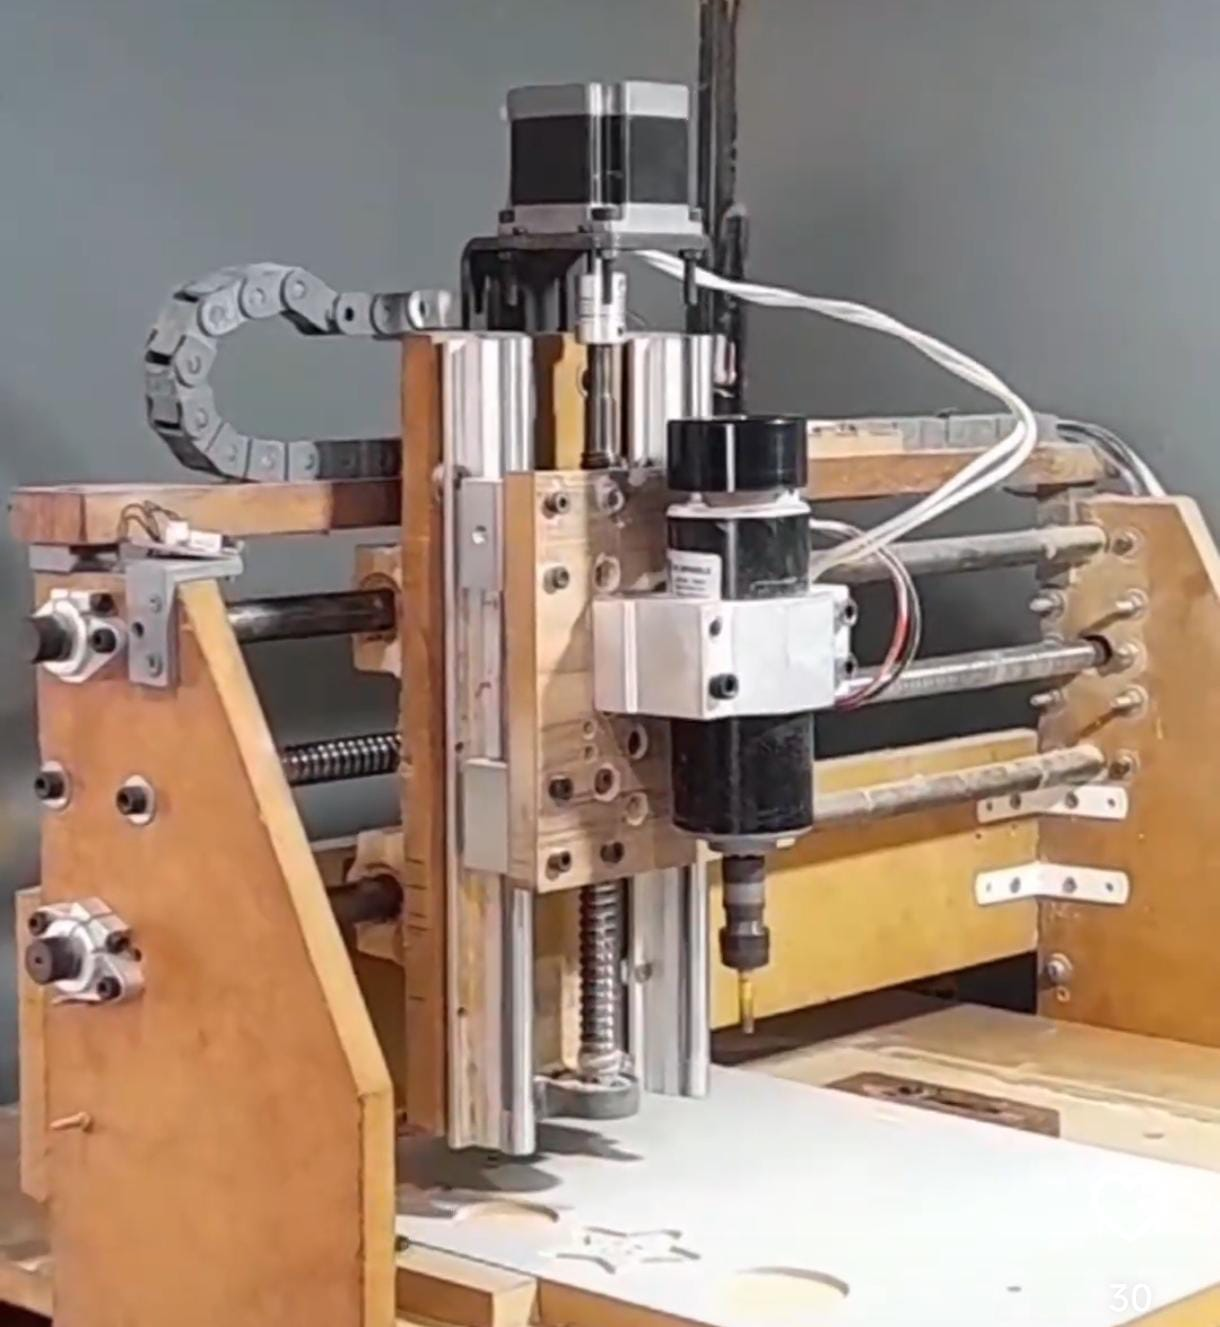
\includegraphics[width=0.5\textwidth,height=\textheight]{D:/Minha pasta/Estudos/UFPA/8º Semestre - 2024.2/Tópico Especiais em Eletrônica/Aluno/Ryan TEE/15.jpeg}

Fig 15: Spindle da Big Fresa.

As fresas, que são as ferramentas de corte, são conectadas ao spindle por um sistema de pinça e rosca. Existem vários tipos de fresa, dependendo do material a ser usinado e da tarefa a ser executada, seja corte, gravação ou furação. Abaixo, você pode ver alguns exemplos de fresas utilizadas no laboratório.

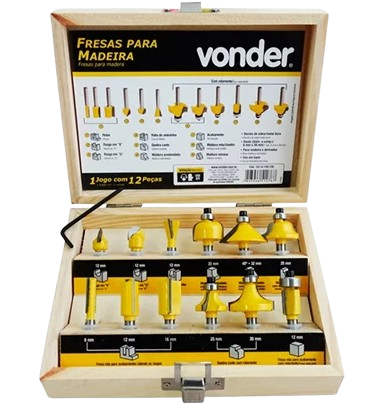
\includegraphics[width=0.6\textwidth,height=\textheight]{D:/Minha pasta/Estudos/UFPA/8º Semestre - 2024.2/Tópico Especiais em Eletrônica/Aluno/Ryan TEE/16.png}

Fig 16: Fresas para madeira.

Para começar a fabricar a peça, é preciso definir a origem de trabalho, levando em conta o sistema de coordenadas tridimensionais. A origem é configurada na parte superior da peça, e conforme o processo avança, a fresa desce no eixo Z negativo, removendo o material até atingir a forma desejada.

\section{Desenho e Controle da Big Fresa}\label{desenho-e-controle-da-big-fresa}

Para gerar o G-code para a Big Fresa, há duas principais opções de software usadas no FABLAB: Fusion 360 e Vectric Aspire. No Fusion 360, você começa modelando a peça em 3D, depois vai para a parte de usinagem, onde escolhe o tipo de fresa e projeta o caminho para a usinagem. Por fim, o arquivo G-code é gerado.

No Vectric Aspire, você pode começar com um desenho 2D vetorizado. No software, você define as ações, como cortes, preenchimentos e furos. Em seguida, ajusta parâmetros como o tipo e o diâmetro da fresa, profundidade de corte, velocidade de movimento, quantidade de passadas e a profundidade de cada passada. O Vectric Aspire também permite simular o processo de usinagem antes de gerar o G-code.

O controle da Big Fresa é feito pelo software UGS (Universal G-code Sender). Com ele, você abre o arquivo G-code e define a posição inicial da área de trabalho. Uma vez configurado, você pode iniciar a usinagem. A interface do UGS também permite controlar a máquina usando joystick, tornando o processo mais prático e intuitivo.

\chapter{SOLDA ELETRÔNICA}\label{solda-eletruxf4nica}

Como monitor da disciplina, eu ensinei os alunos a soldar componentes eletrônicos e a fazer retrabalho. No laboratório, temos equipamentos de qualidade para isso, como ferros de solda, bancadas e uma estação de solda e retrabalho. Essa estação é super útil, com um ferro de solda que permite ajustar a temperatura com precisão através de um potenciômetro; e também contar com um soprador térmico com controle de temperatura e velocidade do ar.

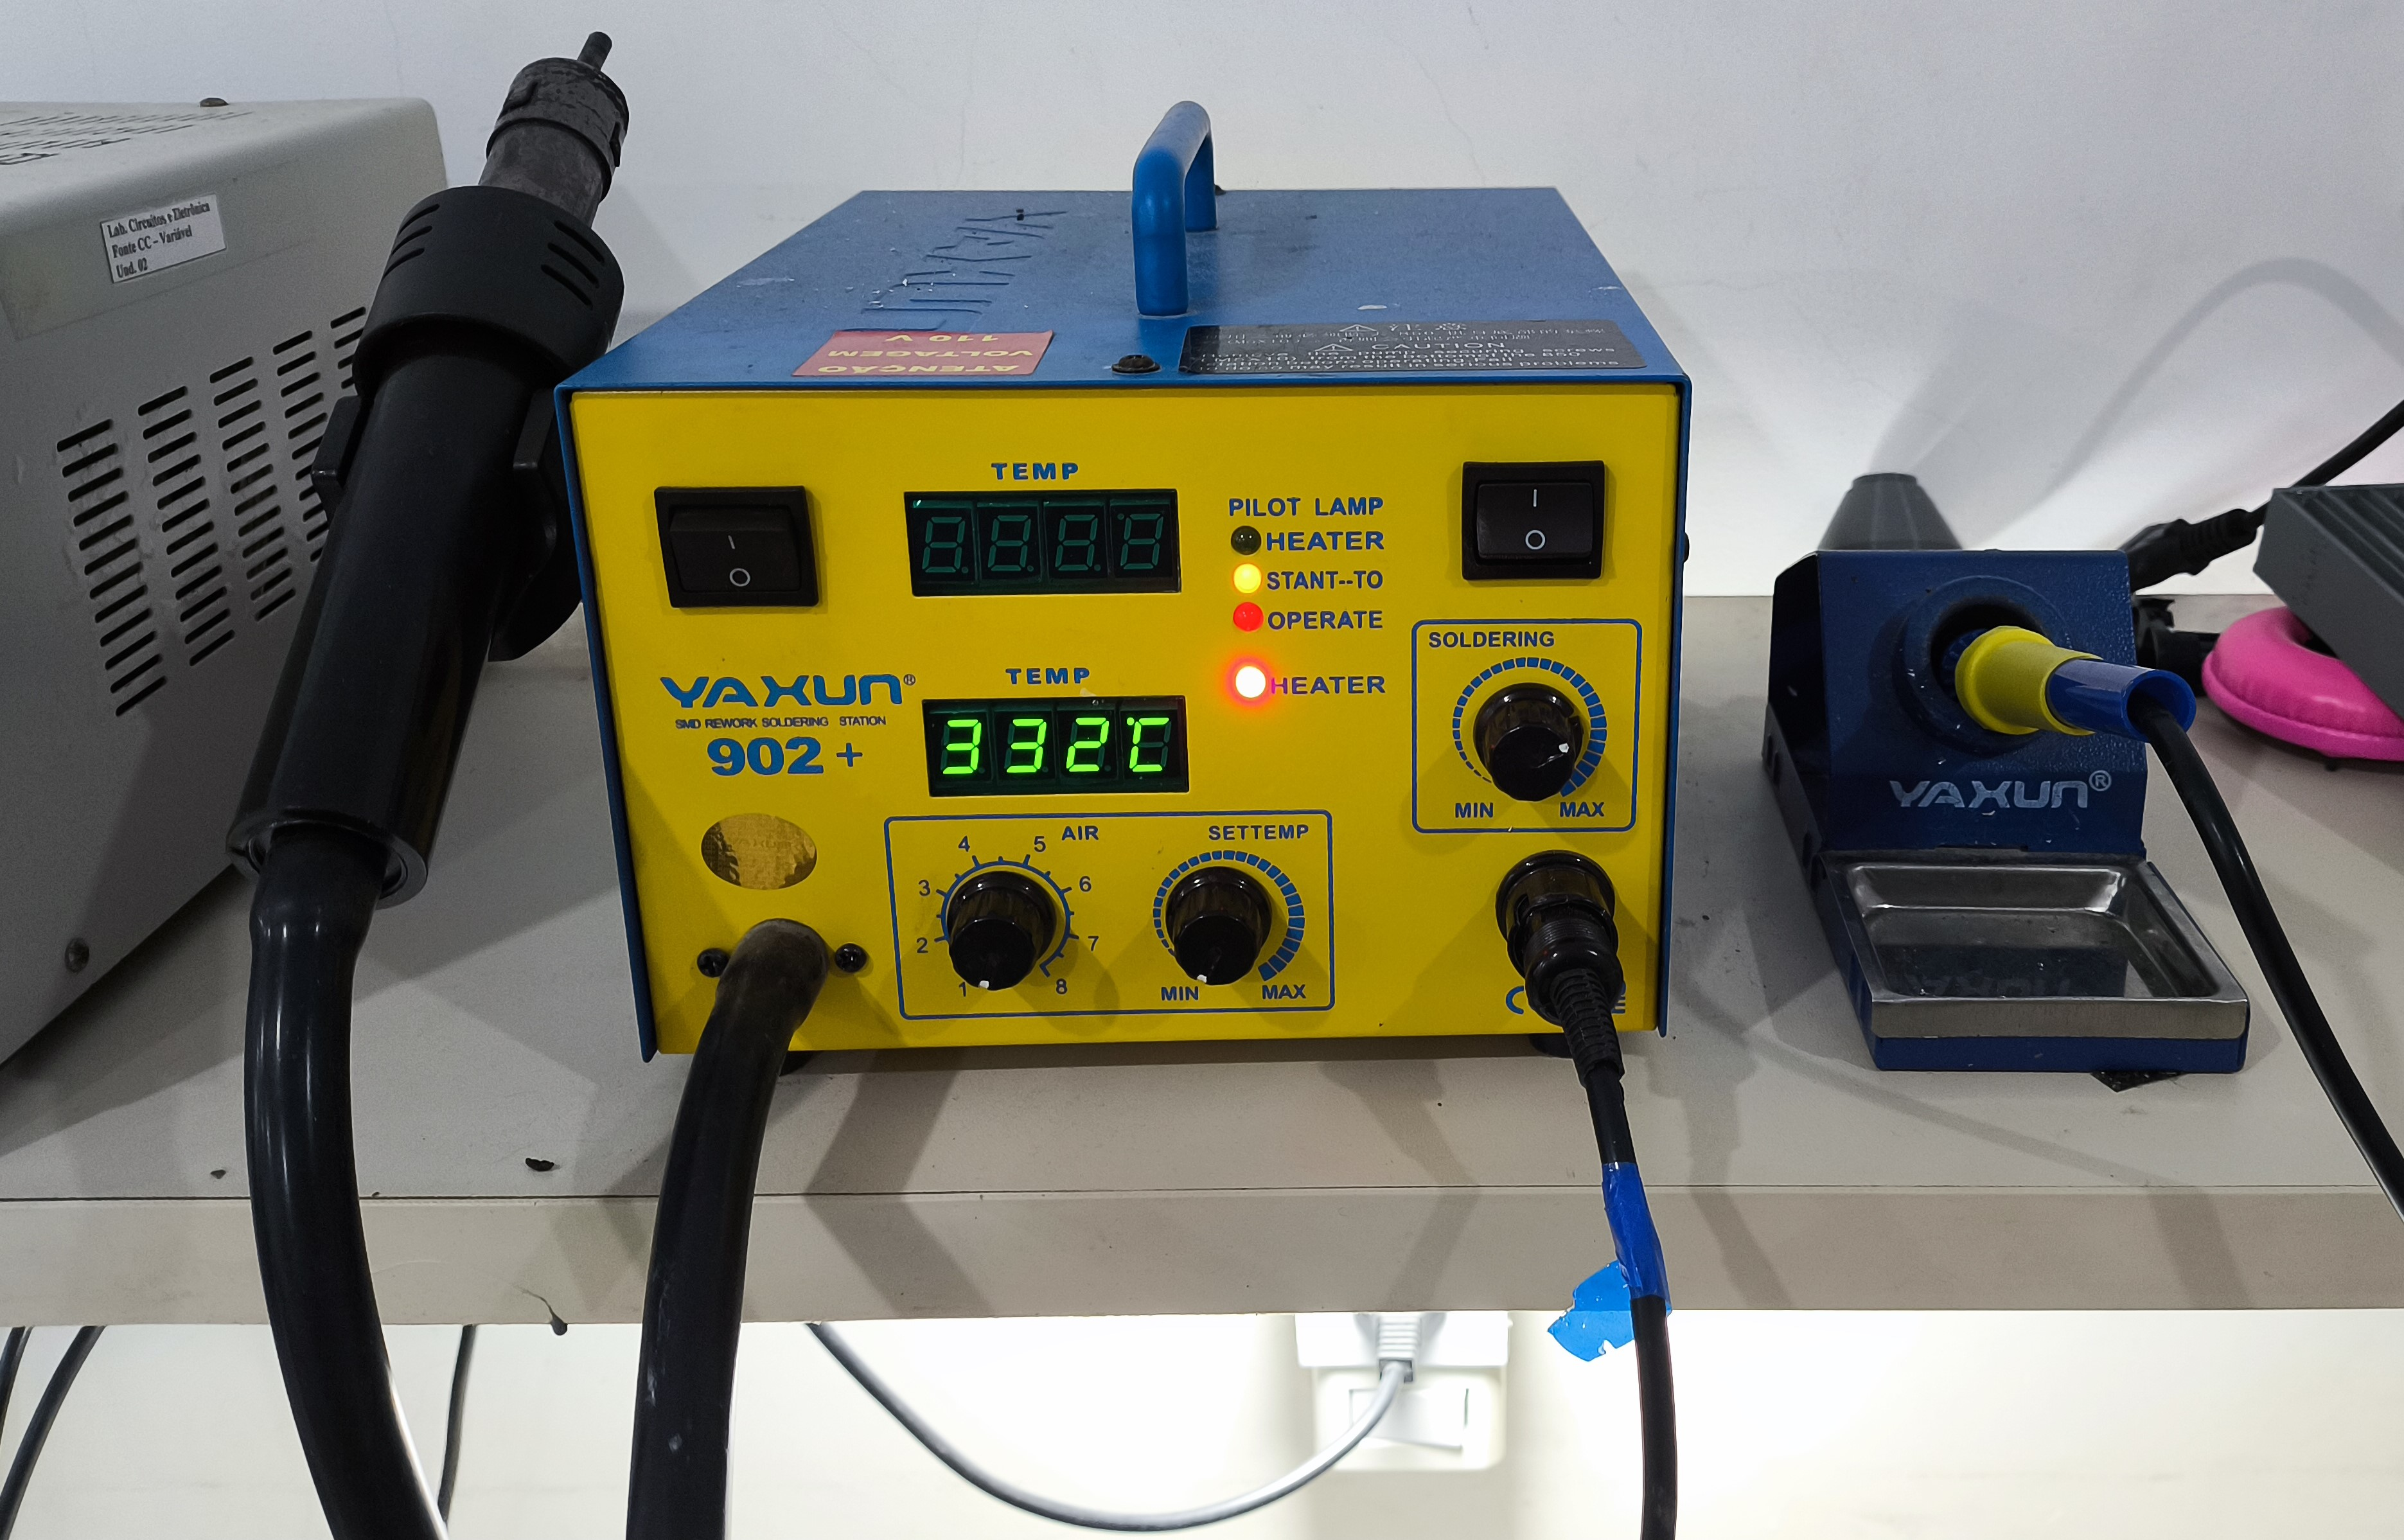
\includegraphics[width=0.6\textwidth,height=\textheight]{D:/Minha pasta/Estudos/UFPA/8º Semestre - 2024.2/Tópico Especiais em Eletrônica/Aluno/Ryan TEE/17.jpg}

Fig 17: Estação de solda e retrabalho.

A soldagem eletrônica une componentes como circuitos integrados, resistores, capacitores, diodos, conectores e outros dispositivos a placas de circuito impresso (PCBs) ou outros substratos. Esse processo cria conexões elétricas e mecânicas que fazem os circuitos funcionarem corretamente. A técnica utiliza um material de solda que é fundido sob calor e, em seguida, solidificado, formando uma junção sólida entre os componentes e os substratos.

Usamos componentes do tipo PTH (Pin Through Hole), que são soldados do outro lado da placa. Eles são mais fáceis de soldar, mas ocupam mais espaço. A solda é feita com estanho, um elemento químico muito usado na eletrônica. Quando o estanho entra em contato com o ferro de solda aquecido, ele derrete e depois endurece, fixando o componente na placa.

No final, pedi para os alunos removerem componentes de uma placa inutilizável e depois soldarem novamente, usando a estação de solda e retrabalho. Ensinei o manuseio correto e seguro das ferramentas, já que tanto o ferro de solda quanto o soprador térmico podem atingir altas temperaturas, suficientes para derreter o estanho, que funde a cerca de 230 °C. Alguns alunos também foram instruídos a fazer furos e soldar em circuitos impressos sem máscara, o que torna o processo um pouco mais complicado, já que a solda pode se espalhar mais facilmente.

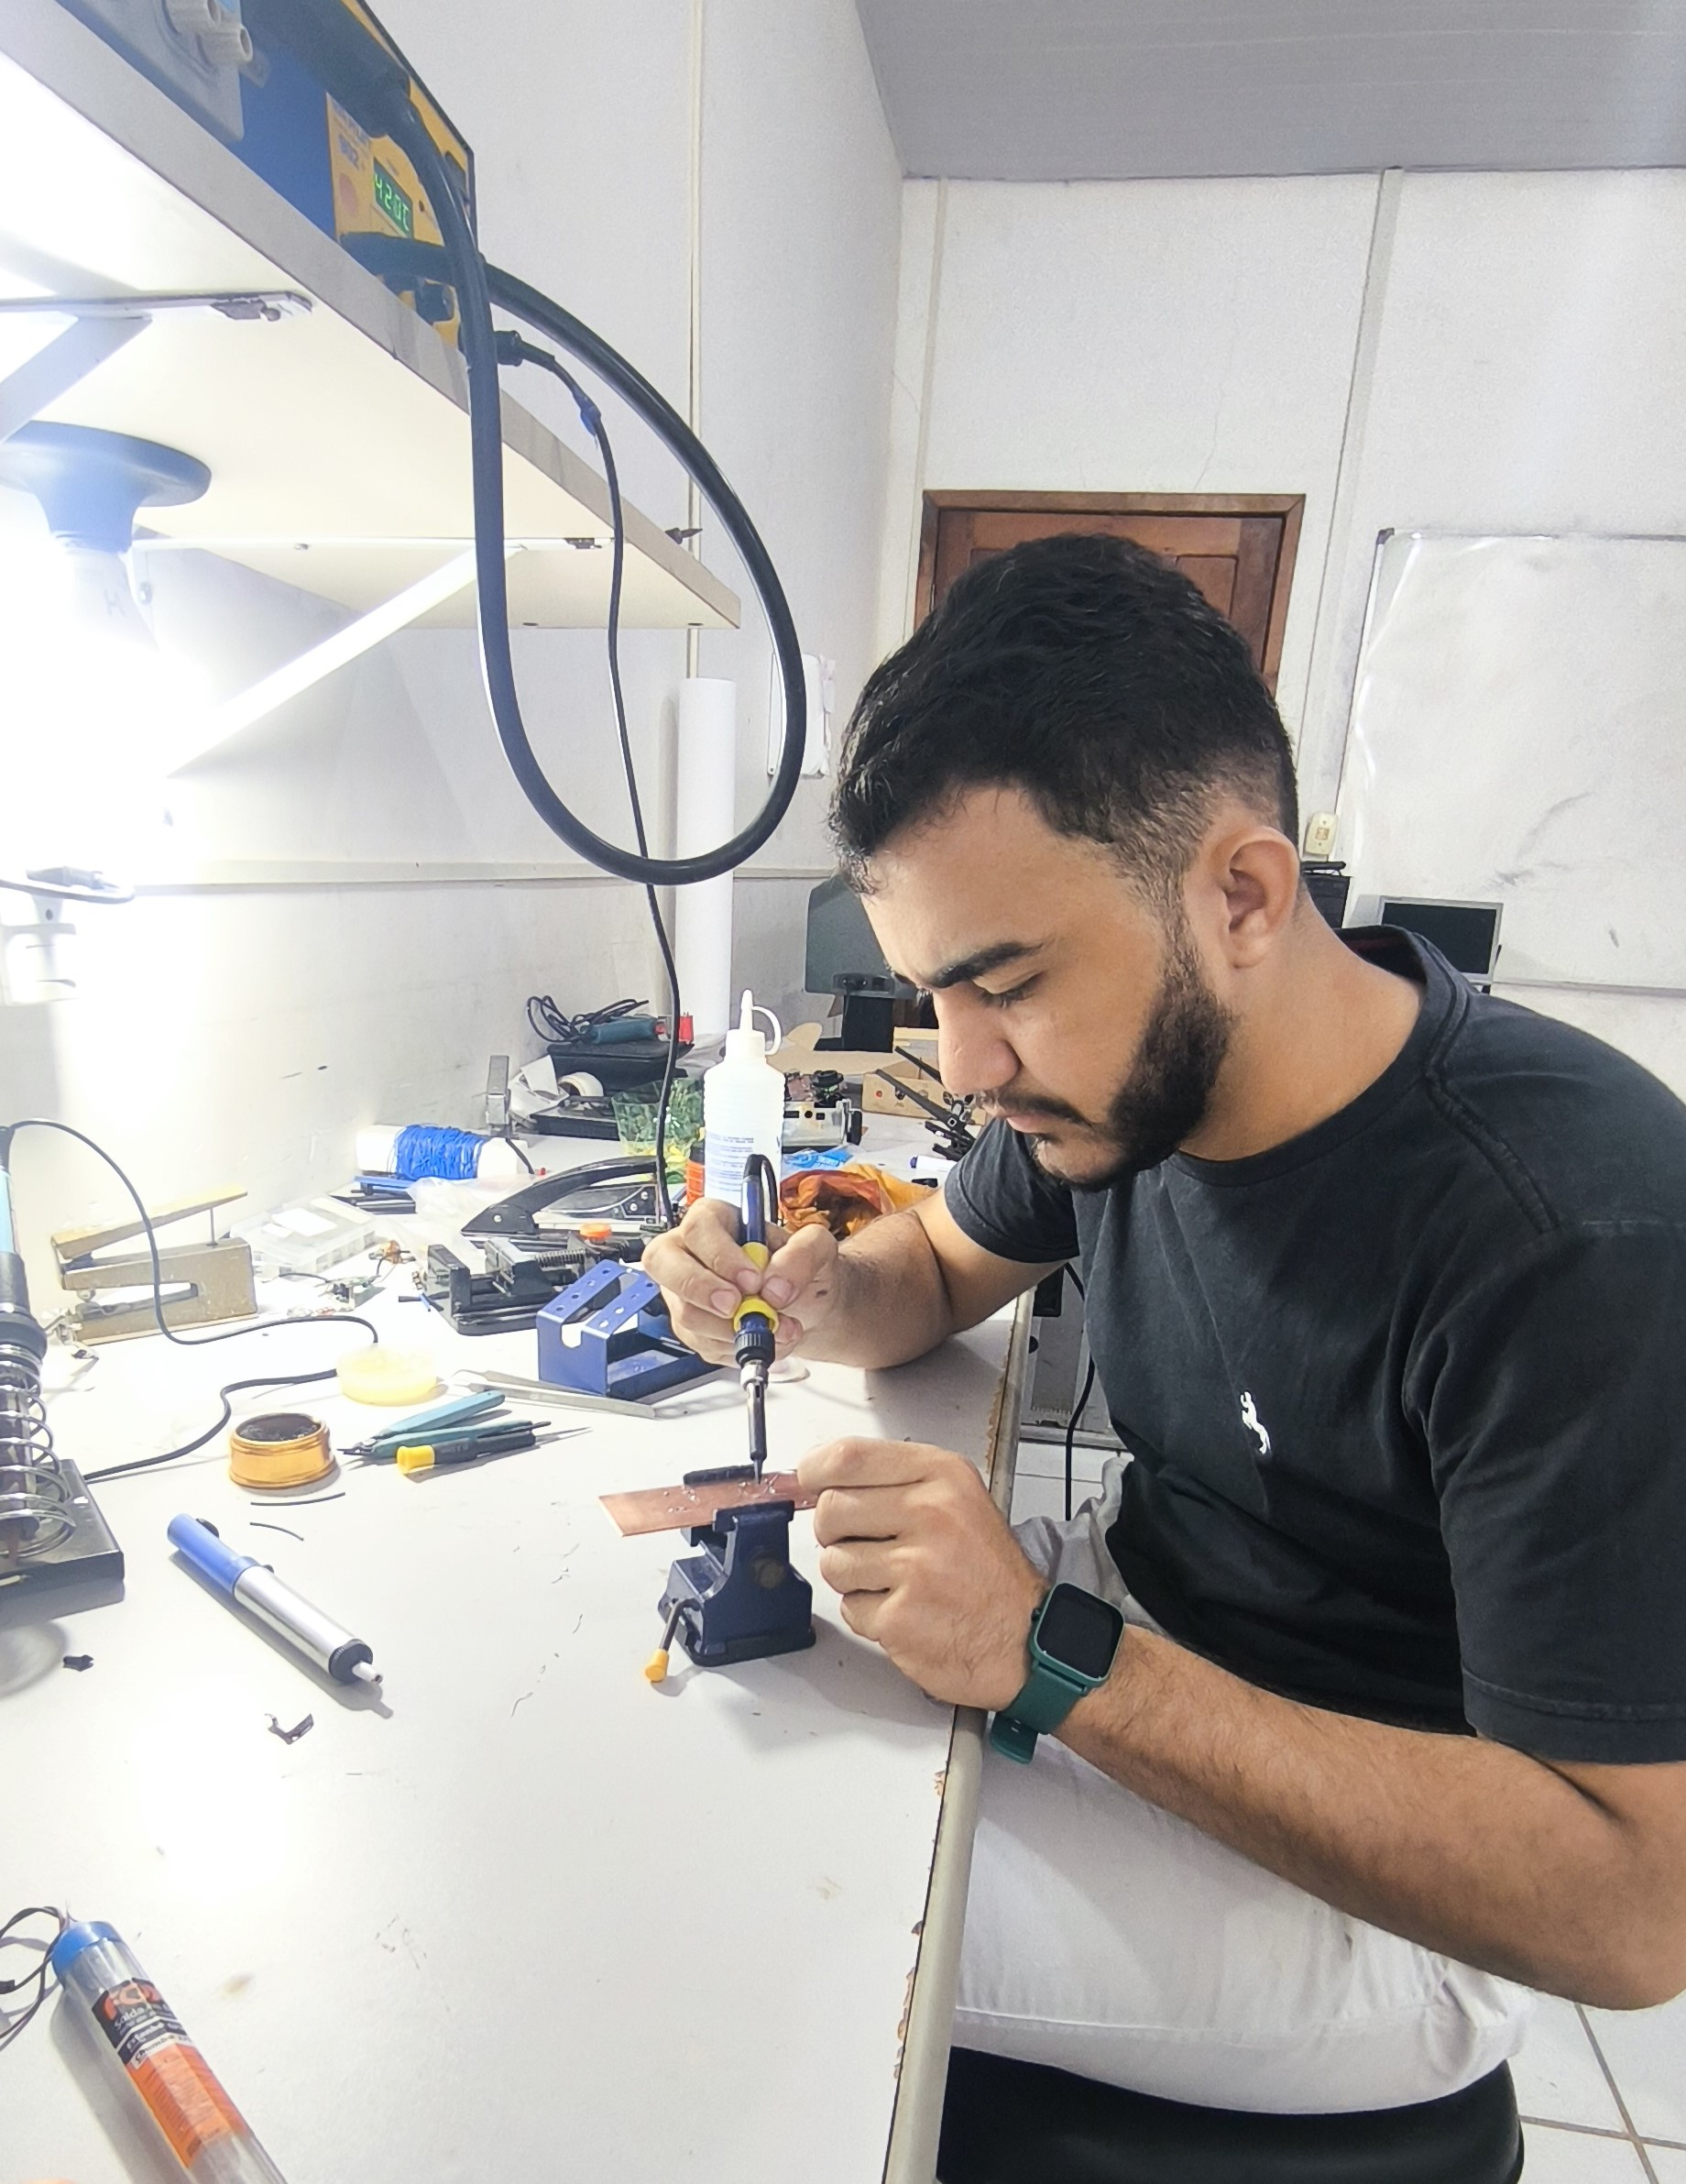
\includegraphics[width=0.5\textwidth,height=\textheight]{D:/Minha pasta/Estudos/UFPA/8º Semestre - 2024.2/Tópico Especiais em Eletrônica/Aluno/Ryan TEE/18.jpg}

Fig 18: Soldando componentes eletrônicos.

\chapter{CIRCUITO IMPRESSO (PCB)}\label{circuito-impresso-pcb}

O projeto e a fabricação de circuitos impressos são essenciais em projetos eletrônicos. O uso da PCB (Placa de Circuito Impresso) traz várias vantagens. Em primeiro lugar, elas garantem a integridade e a confiabilidade do circuito, minimizando o risco de mau contato e falhas intermitentes que podem ocorrer com conexões feitas por jumpers e protoboards. Isso é crucial em projetos que exigem alta confiabilidade e estabilidade operacional.

Além disso, uma PCB bem projetada e fabricada melhora significativamente a estética e a organização do projeto. Componentes dispostos de maneira ordenada e trilhas claramente definidas contribuem para uma montagem mais limpa e profissional. Isso também facilita a manutenção e a modificação do circuito, pois cada componente e conexão está claramente identificado.

No FABLAB, usamos placas de fenolite como material base. Esse material é eletricamente isolante e possui uma camada de cobre na superfície, que conduzirá a eletricidade. Existem dois métodos principais de fabricação de PCBs no laboratório: corrosão e usinagem. Mas, antes de qualquer coisa, é necessário fazer o projeto da PCB.

\section{Projeto do Circuito Impresso}\label{projeto-do-circuito-impresso}

Há várias maneiras de projetar uma PCB, mas utilizamos o site EasyEDA por ser prático e permitir trabalho em equipe. Ele possui uma vasta biblioteca de componentes, facilitando o processo de design. O primeiro passo é criar o diagrama do circuito, garantindo que todos os componentes e conexões estejam corretos. Este diagrama serve como base para a etapa seguinte.

Depois de elaborar o diagrama, passamos para a criação do layout da PCB. Nesta fase, ajustamos as dimensões reais dos componentes e posicionamos cada um deles para evitar que as linhas guia (que representam as trilhas de conexão) se cruzem. Em seguida, escolhemos a largura das trilhas e se o circuito será na parte superior (Top Layer) ou inferior (Bottom Layer). Depois de conectar os componentes com as trilhas, o projeto da PCB está pronto. O formato do arquivo exportado dependerá do método de fabricação que será utilizado.

\section{Fabricação por Corrosão}\label{fabricauxe7uxe3o-por-corrosuxe3o}

O processo de corrosão é mais simples e barato, mas gera resíduos ácidos que precisam ser descartados corretamente. Para demonstrar esse método na aula, fiz um exemplo de circuito utilizando a corrosão. Para produzir a placa, primeiro é necessário exportar o arquivo da PCB no EasyEDA no formato SVG. Esse arquivo é então editado em um software de desenho 2D, como o Inkscape, para obter o negativo da placa, que será gravado a laser.

O próximo passo é cobrir a placa com um material adesivo, como vinil. O laser grava as bordas das trilhas, delineando o contorno delas. Após essa etapa, destacamos os adesivos, deixando apenas as partes das trilhas cobertas, pois o adesivo protegerá essas áreas durante a corrosão.

Para preparar a solução de corrosão, colocamos a placa em um recipiente plástico e adicionamos água até cobrir a placa. Em seguida, retiramos a placa e medimos a quantidade de água no recipiente. A proporção para a solução é de 1 g de percloreto de ferro para cada 4 g de água. Adicionamos o percloreto de ferro à água e misturamos bem.

Com a solução pronta, submergimos a placa e agitamos constantemente para acelerar o processo de corrosão. O ácido corroerá todo o cobre não protegido pelo vinil, deixando apenas as trilhas intactas. Quando o processo estiver completo, lavamos a placa e descartamos a solução corretamente.

Depois disso, retiramos os adesivos das trilhas e perfuramos a placa nos locais necessários. Por fim, soldamos os componentes na PCB, completando o circuito. Embora esse método seja econômico e fácil, é importante manusear os materiais com cuidado e descartar os resíduos de maneira adequada para evitar danos ambientais.

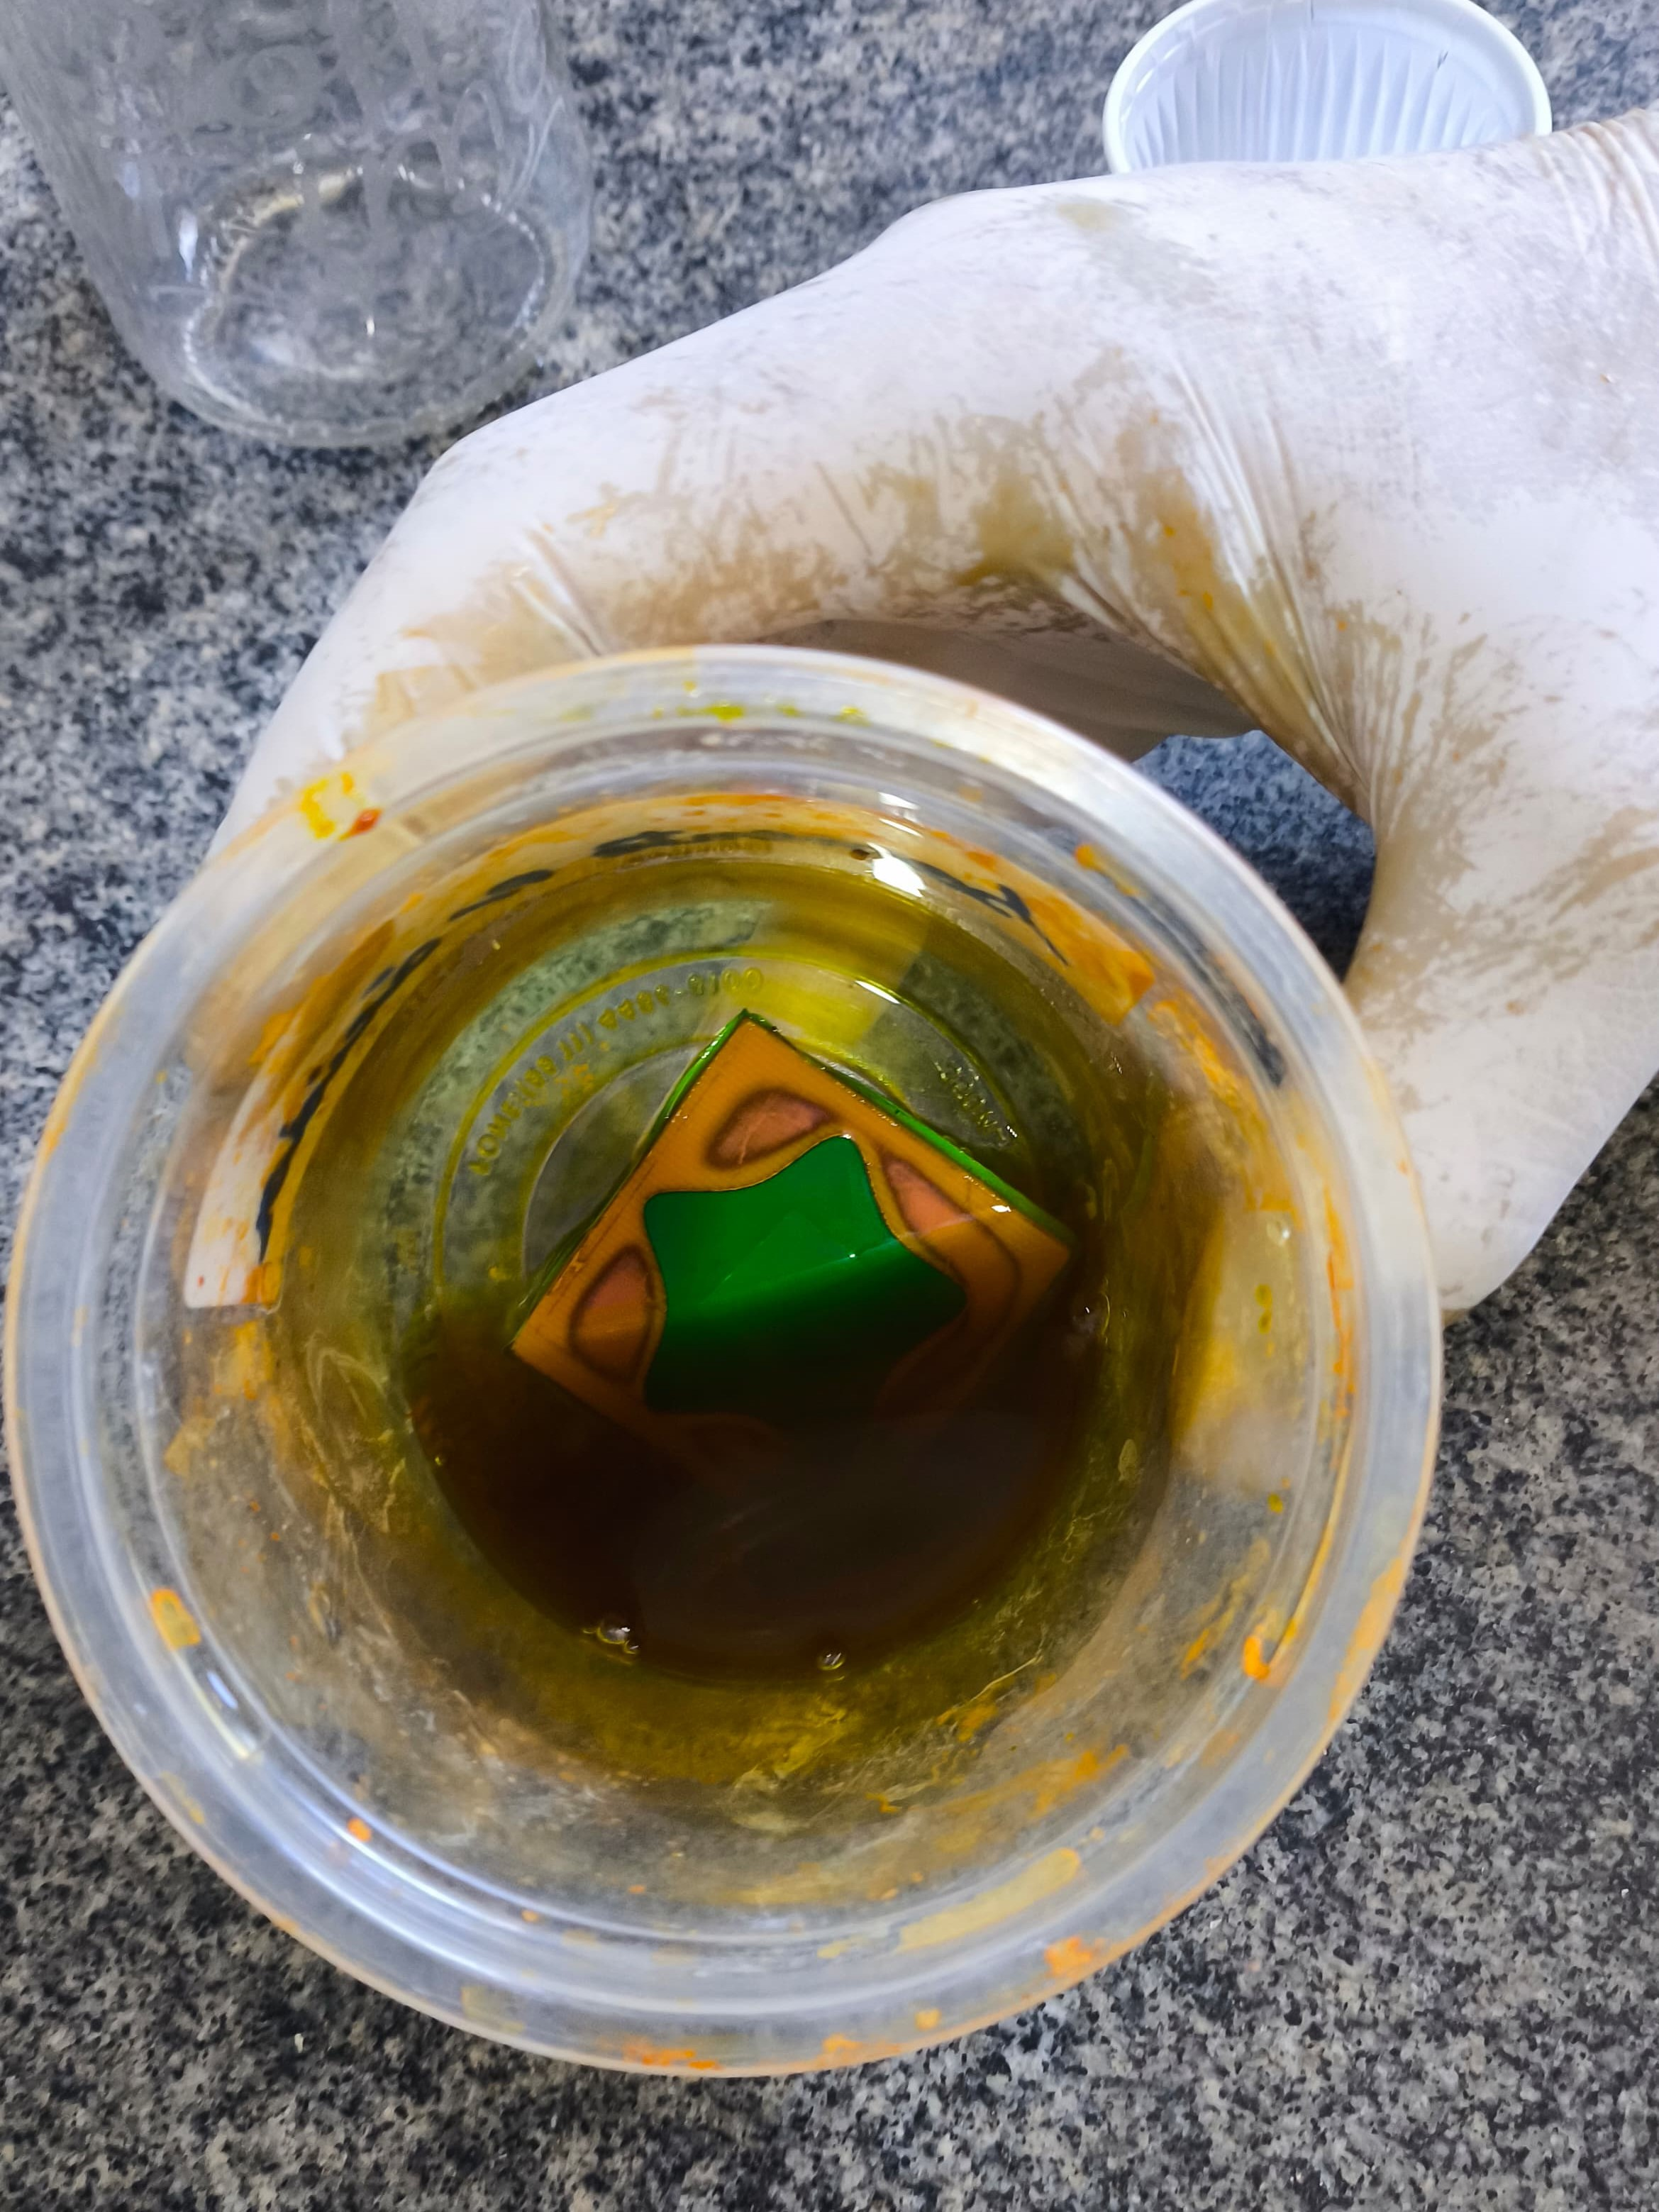
\includegraphics[width=0.4\textwidth,height=\textheight]{D:/Minha pasta/Estudos/UFPA/8º Semestre - 2024.2/Tópico Especiais em Eletrônica/Aluno/Ryan TEE/19.jpeg}

Fig 19: Exemplo de corrosão.

\section{Fabricação por Usinagem}\label{fabricauxe7uxe3o-por-usinagem}

Outro método para fabricar circuitos impressos é através da usinagem. No FABLAB, usamos a CNC fresadora 3018, conhecida como Mini Fresa, que também funciona por processo subtrativo. Seu funcionamento é bem parecido com o da Big Fresa, mas com uma área de trabalho menor e um spindle de menor potência. A Mini Fresa é especialmente focada na produção de PCBs. Infelizmente, ela não foi apresentada para os alunos na disciplina, pois estava em manutenção.

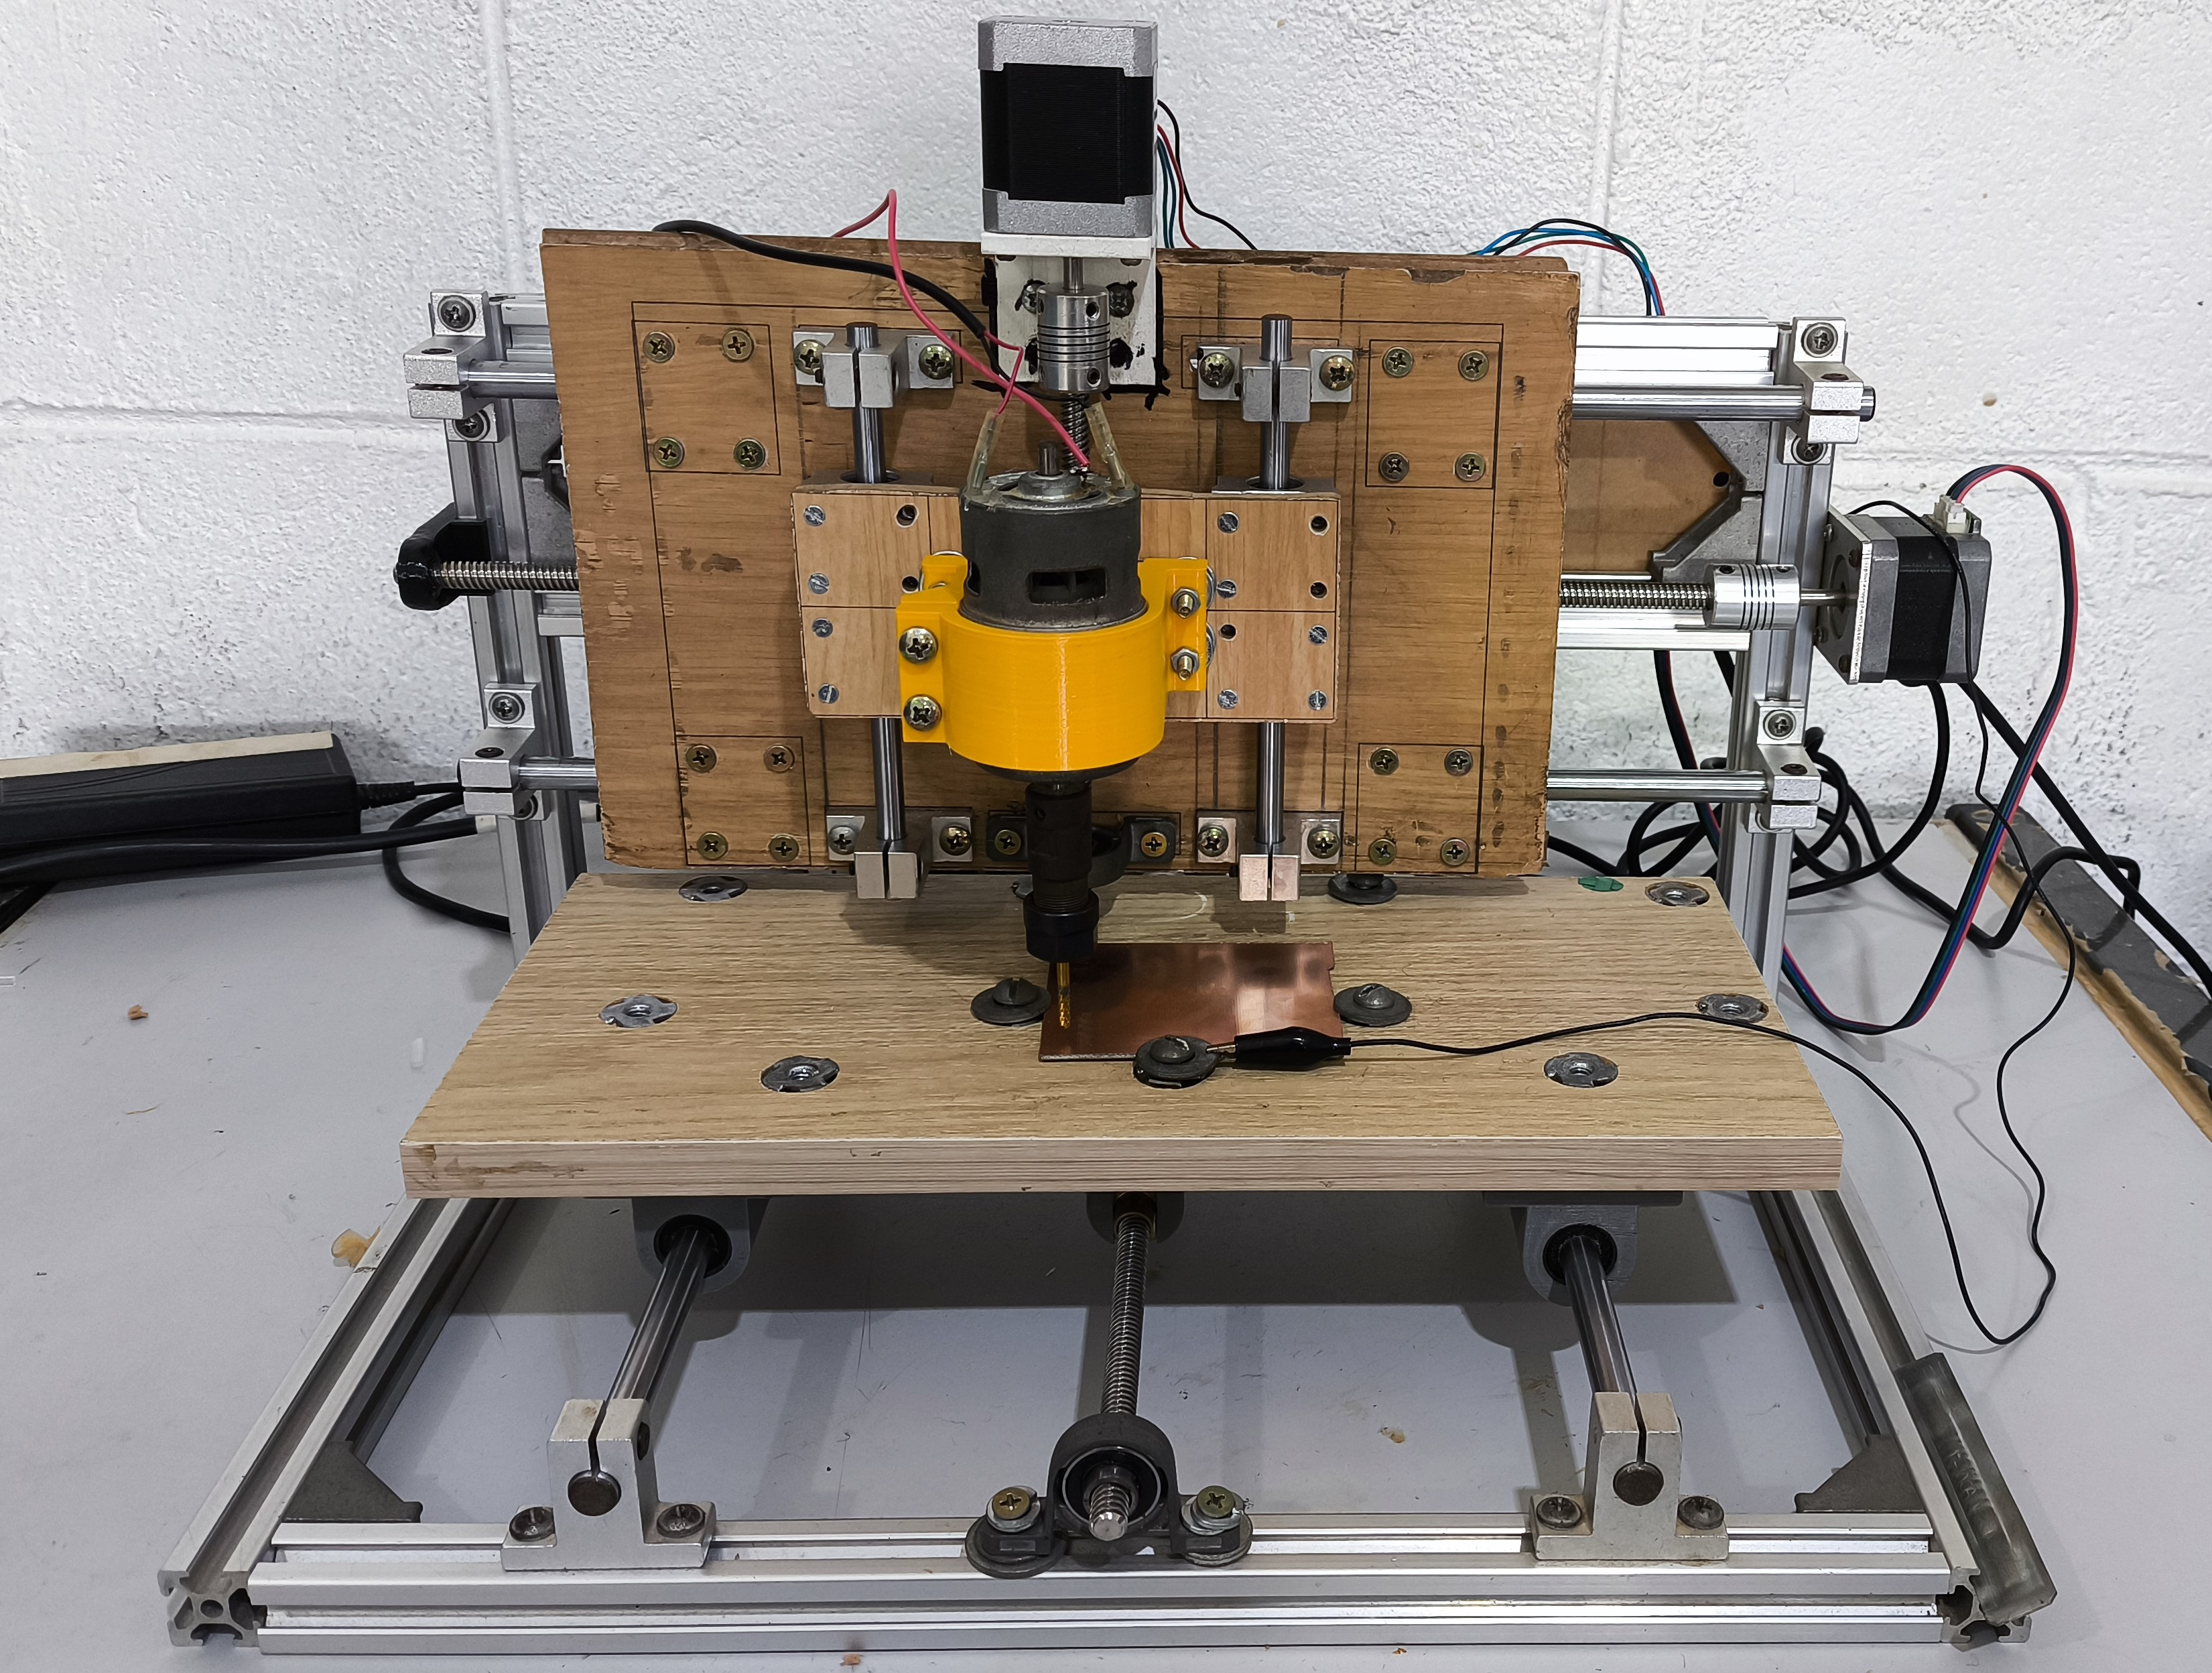
\includegraphics[width=0.6\textwidth,height=\textheight]{D:/Minha pasta/Estudos/UFPA/8º Semestre - 2024.2/Tópico Especiais em Eletrônica/Aluno/Ryan TEE/20.jpg}

Fig 20: Mini fresa.

Para começar a fabricação por usinagem, o primeiro passo é gerar os arquivos Gerber no EasyEDA. Esse processo é bem simples: com o projeto pronto, basta usar a função ``gerar Gerber''. Depois, utilizamos o software FlatCam para definir todos os parâmetros necessários para a fabricação. Normalmente, escolhemos três ações que geram três G-codes diferentes: um para as trilhas, um para os furos e outro para o corte das bordas do circuito. Para cada ação, é preciso definir parâmetros como o tipo de fresa a ser usada, a profundidade de corte, a velocidade de movimentação, a quantidade de passadas, entre outros.

O controle da Mini Fresa é feito pelo software Candle GRBL, que é bem parecido com o UGS usado na Big Fresa. Ambos os softwares podem controlar os dois tipos de fresadoras. Antes de iniciar o trabalho, escolhemos a fresa apropriada e definimos a origem da área de trabalho. O Candle realiza um mapeamento de alturas da área de trabalho para ajustar a altura da fresa em relação ao material, utilizando o princípio de continuidade elétrica para essa medição.

Uma vez configurado, o processo de usinagem começa. Cada vez que um arquivo Gerber é trocado, é necessário substituir a fresa correspondente. Esse método é mais caro e demorado, mas tem a vantagem de não gerar resíduos tóxicos. Por outro lado, ele gera bastante pó, o que requer cuidados adicionais para manter o ambiente limpo.

\chapter{PLOTTER}\label{plotter}

Outra máquina apresentada na disciplina foi a plotter, ideal para cortes de alta precisão em diversos materiais, como papel, acetato, vinil, entre outros. Na demonstração, utilizamos vinil, onde a máquina realiza cortes usando uma agulha bem fina. Para isso, o arquivo que precisa ser enviado para ela deve estar no formato PNG.

A plotter possui um carrinho que se move lateralmente e uma lâmina que faz os cortes no material. É possível usar diferentes tipos de lâminas, dependendo da espessura e textura do material. Por exemplo, lâminas mais afiadas são ideais para cortes detalhados em materiais finos, enquanto lâminas mais robustas são usadas para materiais mais espessos.

O software utilizado para controlar a plotter converte as linhas dos desenhos em comandos específicos, definindo o caminho que a máquina vai percorrer. Ele também ajusta os parâmetros do processo, como a velocidade de corte e a profundidade que a agulha deve perfurar. Além disso, o software permite escolher entre cortes contínuos ou ponteados, dependendo do resultado desejado.

Durante a aula, destacamos algumas vantagens da plotter. Ela permite cortes precisos e detalhados, que seriam difíceis de fazer manualmente. Isso é especialmente útil para projetos que exigem repetição e consistência, como adesivos personalizados e modelos para artesanato. Também mencionamos a importância de ajustar corretamente os parâmetros de corte para evitar danificar o material ou a lâmina.

A plotter não só agiliza o processo de corte, como também aumenta a qualidade e a precisão dos trabalhos, permitindo aos alunos explorar diversas possibilidades criativas e profissionais em seus projetos. Ao final da demonstração, os alunos puderam experimentar a máquina, criando seus próprios designs em vinil, e aprendendo na prática como ajustar os parâmetros para obter os melhores resultados.

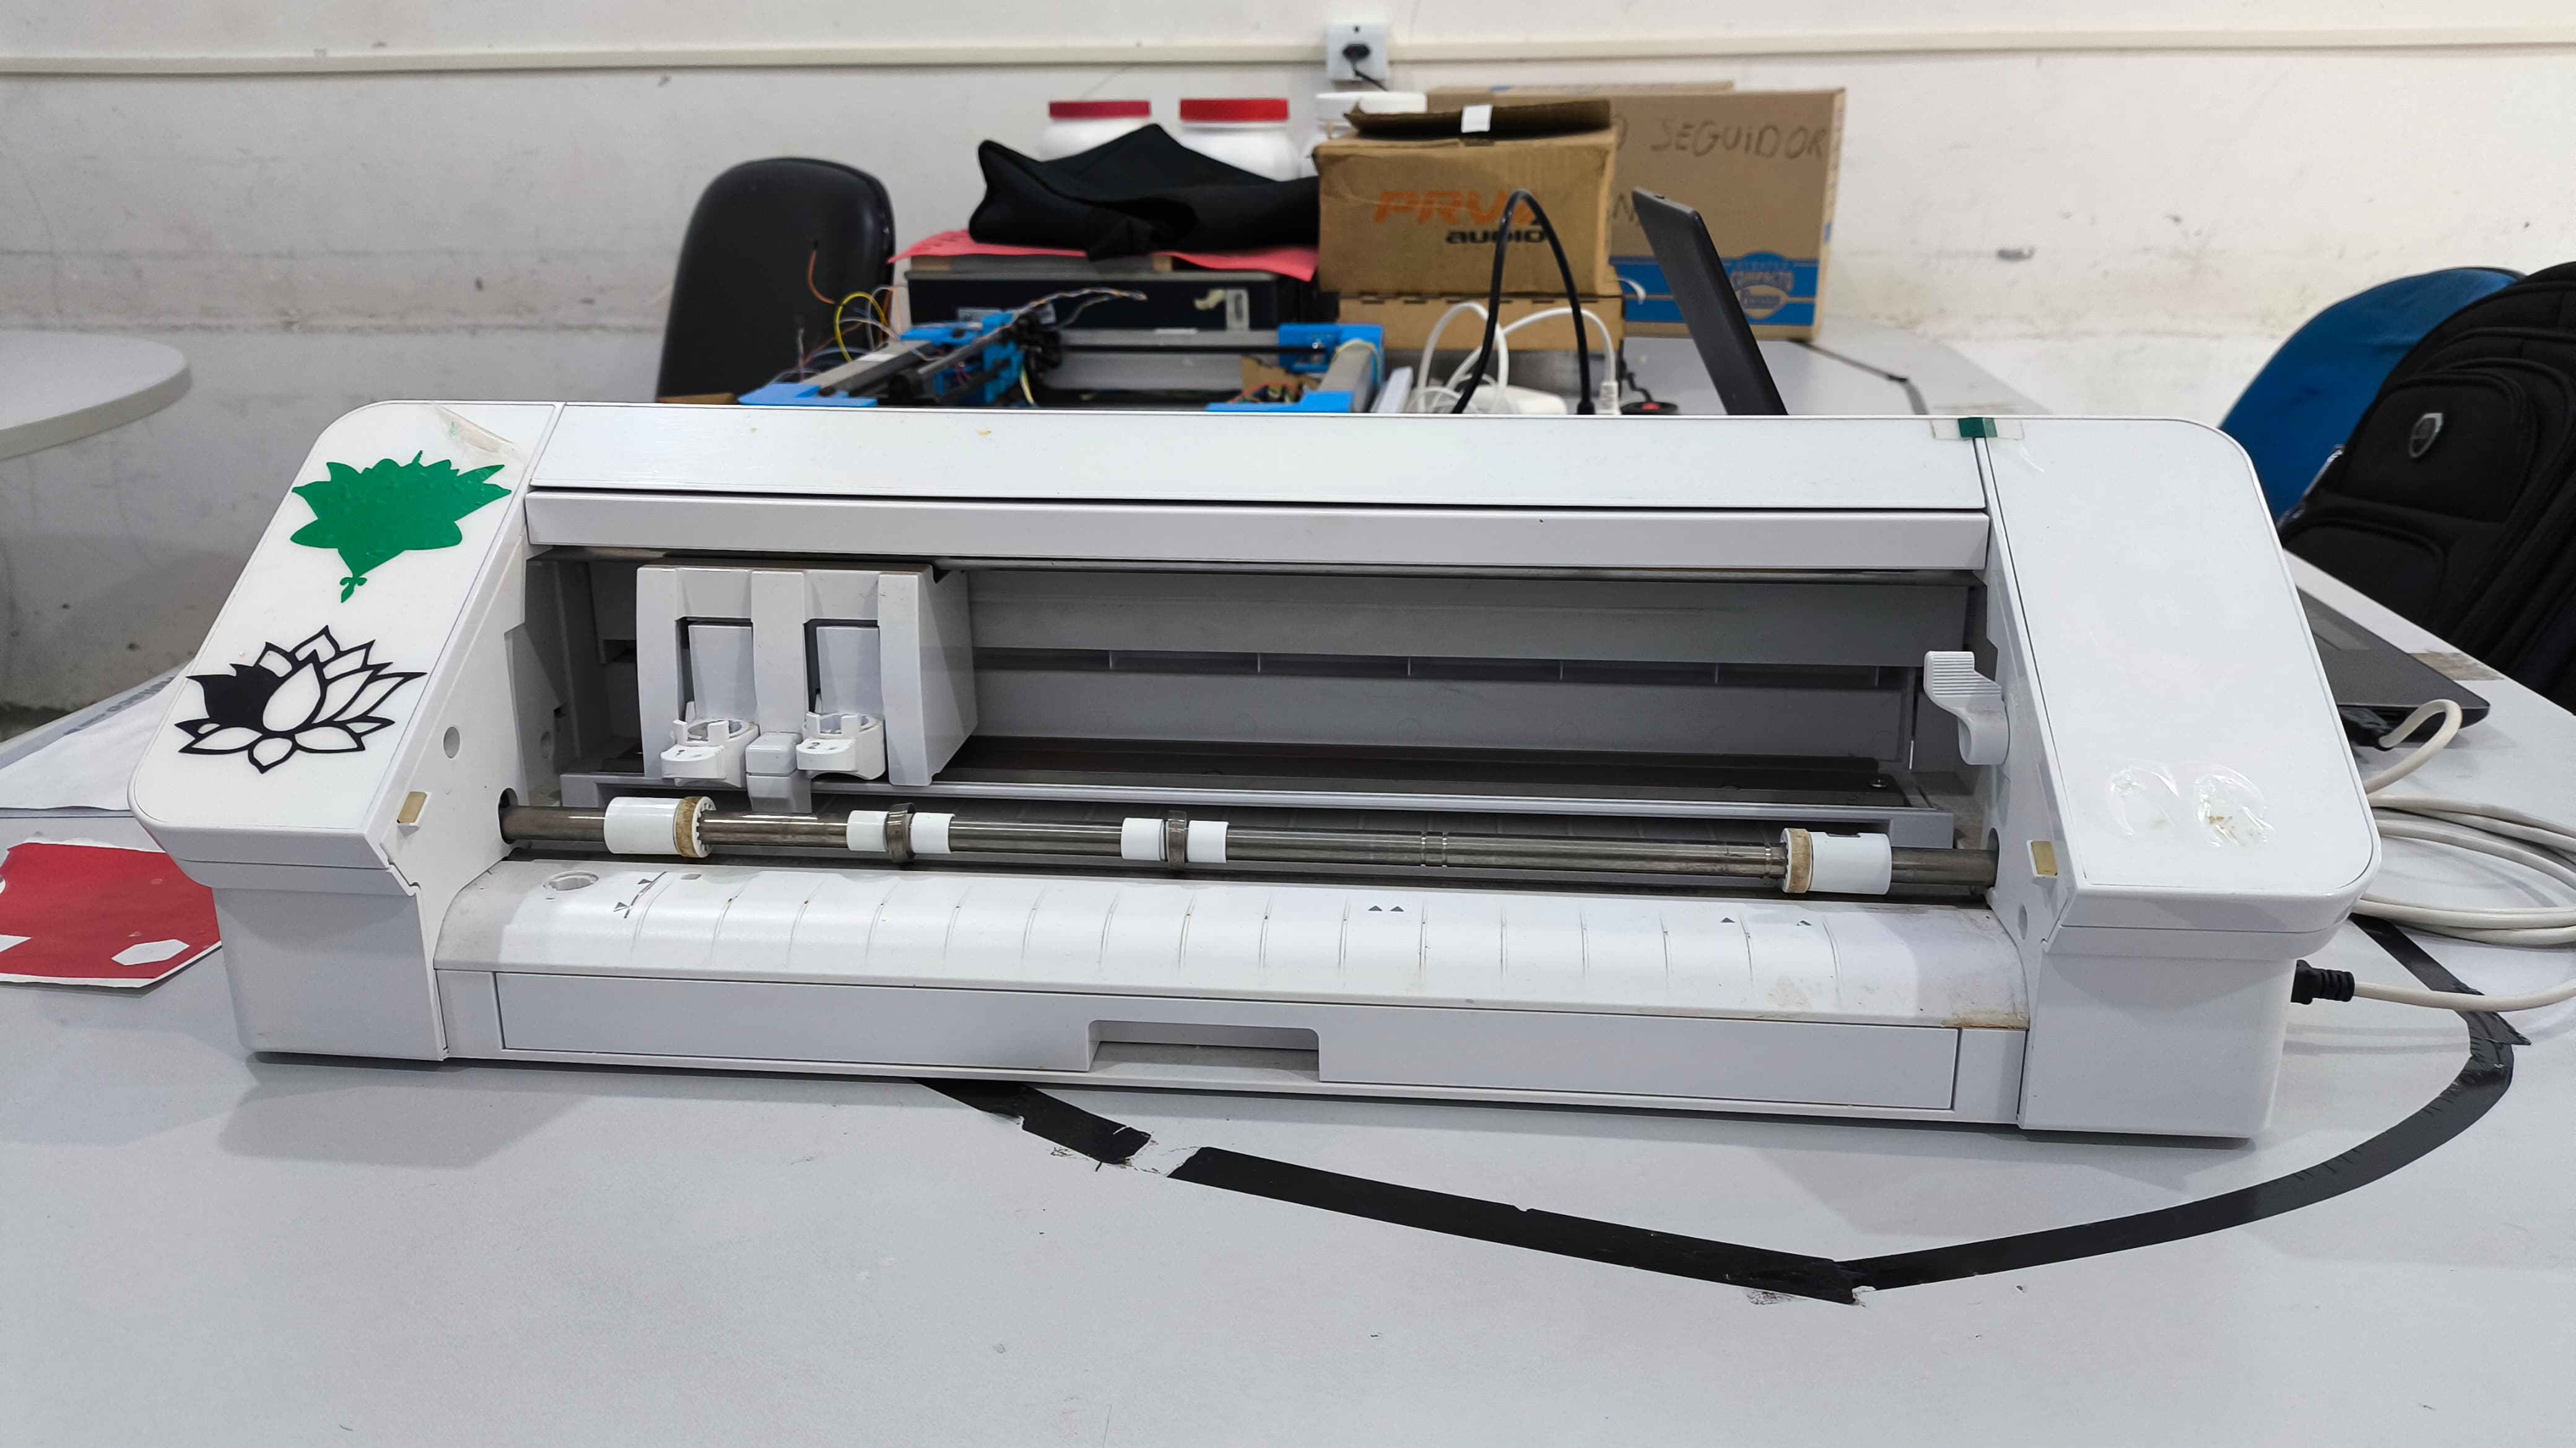
\includegraphics[width=0.6\textwidth,height=\textheight]{D:/Minha pasta/Estudos/UFPA/8º Semestre - 2024.2/Tópico Especiais em Eletrônica/Aluno/Ryan TEE/21.jpeg}

Fig 21: Plotter.

\chapter{PROGRAMAÇÃO EM ARDUINO}\label{programauxe7uxe3o-em-arduino}

Também tivemos uma aula sobre programação em Arduino, onde abordamos os conceitos básicos, como funciona a plataforma, e os diferentes tipos de Arduinos disponíveis. Falamos sobre os modelos mais populares, como o Arduino Uno, Mega e o Nano, cada um com suas especificidades e aplicações ideais.

\section{Tipos de Arduino:}\label{tipos-de-arduino}

Arduino Uno: O mais comum e recomendado para iniciantes. Tem 14 portas digitais e 6 analógicas.

Arduino Mega: Ideal para projetos que exigem muitas entradas e saídas, com 54 portas digitais e 16 analógicas.

Arduino Nano: Menor e mais compacto, perfeito para projetos que precisam economizar espaço.

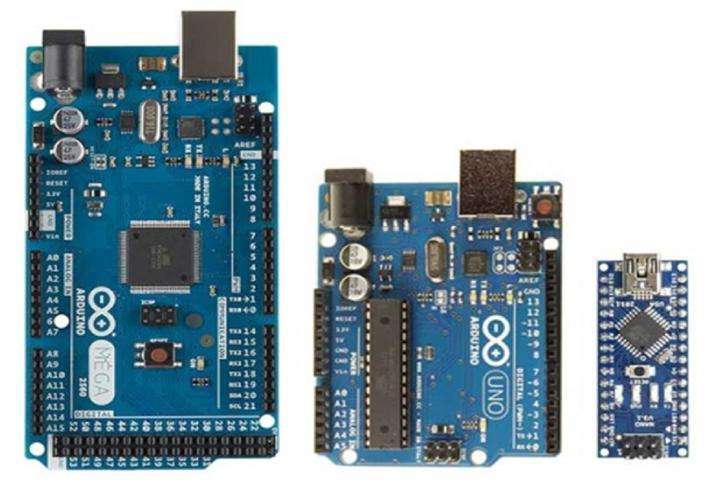
\includegraphics[width=0.45\textwidth,height=\textheight]{D:/Minha pasta/Estudos/UFPA/8º Semestre - 2024.2/Tópico Especiais em Eletrônica/Aluno/Ryan TEE/40.png}

Fig 22:Tipos de Arduinos.

\section{Funcionamento das Portas:}\label{funcionamento-das-portas}

Portas Digitais: Utilizadas para ler ou enviar sinais digitais, ou seja, valores de 0 ou 1 (LOW ou HIGH). Essas portas podem ser configuradas como entrada (INPUT) ou saída (OUTPUT).

Portas Analógicas: Utilizadas para ler valores analógicos variáveis, geralmente de 0 a 1023. Essas portas são essenciais para ler sensores que fornecem valores não digitais, como potenciômetros.

PWM (Pulse Width Modulation): Algumas portas digitais têm a capacidade de emitir sinais PWM, que são úteis para controlar dispositivos como motores e LEDs com variação de intensidade. No Arduino Uno, por exemplo, as portas 3, 5, 6, 9, 10 e 11 têm essa função.

Portas de Comunicação Serial (TX/RX): Utilizadas para comunicação serial, essencial para a transferência de dados entre o Arduino e outros dispositivos, como computadores ou outros microcontroladores.

Também foi apresentada a IDE do Arduino, que é a interface onde você escreve, compila e carrega os códigos (sketches) no microcontrolador. Para tornar a aula mais prática, foi ensinado como fazer alguns códigos básicos, como ligar um LED.

\chapter{PROJETO FINAL}\label{projeto-final}

Meu projeto final foi inspirado no clássico jogo Genius, que desafia os jogadores a memorizarem sequências de cores e sons. Originalmente, o jogo possuía botões coloridos que emitiam sons harmônicos e se iluminavam em sequência, e a tarefa era repetir essa sequência sem cometer erros. A segui temos as etapas do projeto.

\section{Planejamento e Conceito:}\label{planejamento-e-conceito}

Para começar, estudei como o jogo funcionava. Com base nos materiais disponíveis, decidi usar um Arduino Nano para controlar tudo. Optei por quatro botões, cada um com um LED de cor correspondente, e um buzzer para os sons. O buzzer foi escolhido por sua capacidade de alterar o som pela sua frequência, o que permite controlar os tons através do Arduino.

\section{Montagem e Testes na Protoboard:}\label{montagem-e-testes-na-protoboard}

A primeira etapa foi montar e testar o circuito na protoboard. Isso facilitou a montagem inicial do circuito, possibilitando ajustes e testes conforme avançava no projeto.

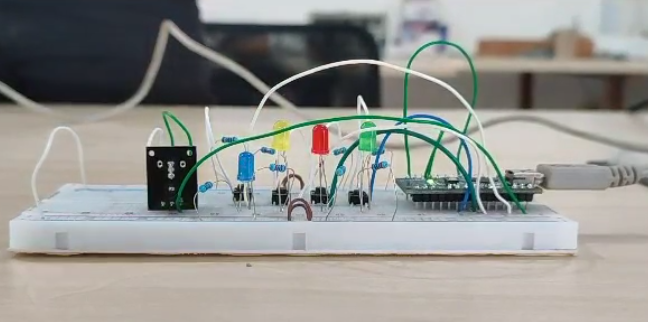
\includegraphics[width=0.6\textwidth,height=\textheight]{D:/Minha pasta/Estudos/UFPA/8º Semestre - 2024.2/Tópico Especiais em Eletrônica/Aluno/Ryan TEE/22.png}

Fig 23: Circuito na Protoboard.

\section{Explicação do Código:}\label{explicauxe7uxe3o-do-cuxf3digo}

Definição de Notas e Melodia: No início do código, são definidas as notas musicais que serão usadas na melodia do jogo. Cada nota tem um valor associado que representa sua frequência sonora e uma duração que indica por quanto tempo ela deve ser tocada.

Setup() - Configuração Inicial:

A função setup() é responsável por configurar o ambiente inicial do jogo.

Inicia a comunicação serial para debug (Serial.begin(9600)).

Gera uma semente aleatória para gerar a sequência de cores e sons (randomSeed(analogRead(0))).

Define os pinos dos LEDs e do buzzer como saídas (pinMode()).

Em seguida, reproduz a melodia definida no início do jogo usando o buzzer, tocando cada nota na sequência.

Loop() - Execução Contínua:

O loop principal (loop()) do programa continua executando repetidamente enquanto o Arduino estiver ligado.

Dentro deste loop, o código verifica constantemente as ações do jogador e controla a sequência de LEDs e sons para o jogo.

\section{Funcionamento do Jogo:}\label{funcionamento-do-jogo}

Geração da Sequência: Uma sequência aleatória de LEDs é gerada e mostrada para o jogador através de piscadas e sons correspondentes.

Entrada do Jogador: O jogador deve repetir a sequência pressionando os botões corretos na ordem correta.

Feedback Visual e Sonoro: Cada botão pressionado acende o LED correspondente e emite um som característico através do buzzer.

Verificação de Acertos: O programa verifica se a sequência de botões pressionados pelo jogador corresponde à sequência gerada aleatoriamente.

Final do Jogo: Se o jogador errar a sequência, o jogo reinicia, mostrando uma animação e emitindo sons indicando o fim do jogo.

\section{Idealização do produto final}\label{idealizauxe7uxe3o-do-produto-final}

Após conseguir fazer o circuito funcionar e finalizar o código, o próximo passo foi planejar o projeto final do Genius, pensando em transformá-lo em um produto completo. Isso envolveu decidir a disposição dos botões e LEDs, como integrar o circuito com o Arduino e planejar a alimentação de todo o sistema.

A ideia central foi criar uma caixa para o jogo. Na parte superior da caixa, seria colocada uma superfície onde os botões poderiam ser pressionados. Cada botão seria acompanhado por dois LEDs, totalizando 8 LEDs de 4 cores diferentes. O Arduino ficaria na parte inferior da caixa, alimentado por uma bateria de 9 volts.

Para manter os botões separados da placa principal do Arduino e reduzir a necessidade de muitos jumpers (fios de conexão), foi necessário criar um circuito para cada botão. Cada circuito incluiu os dois LEDs associados ao botão, além de dois resistores separados, um para os LEDs e outro para o botão.

\section{Projeto do Circuito Impresso (PCB):}\label{projeto-do-circuito-impresso-pcb}

Após isso foi necessário fazer o diagrama das conexões elétricas no EasyEDA, de modo para fazer o circuito impresso.

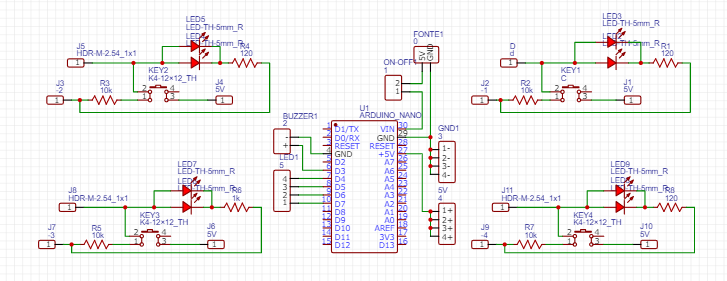
\includegraphics[width=0.5\textwidth,height=\textheight]{D:/Minha pasta/Estudos/UFPA/8º Semestre - 2024.2/Tópico Especiais em Eletrônica/Aluno/Ryan TEE/23.png}

Fig 24: Esquemático elétrico.

Depois de finalizar o diagrama das conexões elétricas no EasyEDA, o próximo passo foi transformá-lo em um projeto de circuito impresso (PCB). Uma das principais dificuldades foi organizar os componentes de forma compacta e eficiente para facilitar as interconexões. Isso foi crucial para garantir que o circuito funcionasse corretamente e ocupasse o menor espaço possível na placa.
Após planejar a disposição dos componentes, foi feita a conexão das trilhas e o layout final da placa, como mostrado na figura a seguir.

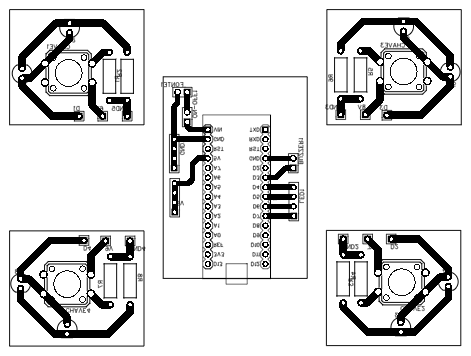
\includegraphics[width=0.4\textwidth,height=\textheight]{D:/Minha pasta/Estudos/UFPA/8º Semestre - 2024.2/Tópico Especiais em Eletrônica/Aluno/Ryan TEE/24.png}

Fig 25: Representação da PCB.

No EasyEDA também é possível obter um a visualização do circuito em 3D, como visto na imagem a seguir.

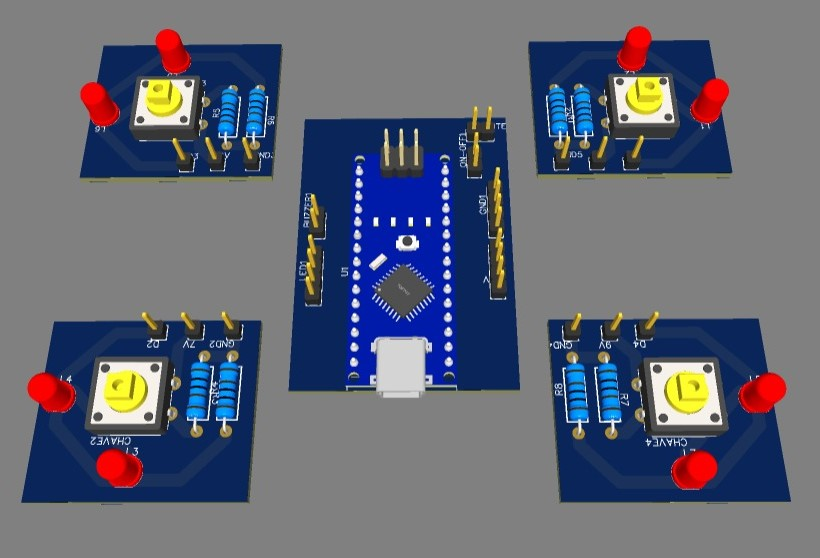
\includegraphics[width=0.4\textwidth,height=\textheight]{D:/Minha pasta/Estudos/UFPA/8º Semestre - 2024.2/Tópico Especiais em Eletrônica/Aluno/Ryan TEE/25.jpeg}

Fig 26: Representação da PCB em 3D.

\section{Fabricação do Circuito Impresso:}\label{fabricauxe7uxe3o-do-circuito-impresso}

Para fazer a fabricação das placas eu optei por fazer através do método de corrosão, pois a fresadora 3018 ainda estava em fase de manutenção. Então para isso foi necessário exporta o arquivo em SVG, e abrir ele no Inkscape, fazendo as devidas configurações, colocando o contorno nas trilhas, para que o laser passasse. Após isso foi cortado pedaços de fenolites cobreados na superfície, e colocado o vinil adesivo; e posteriormente levado ao laser para destacar as trilhas das placas, utilizando o laser com uma potência de 8\%. No final obtive as placas e destaquei o vinil onde foi cortado e deixei só a parte das trilhas.

Depois disso preparei a solução para corrosão, utilizando percloreto de ferro e água, sendo na proporção de 1 para 4 respectivamente, de maneira obtiver as placas de circuitos impresso.

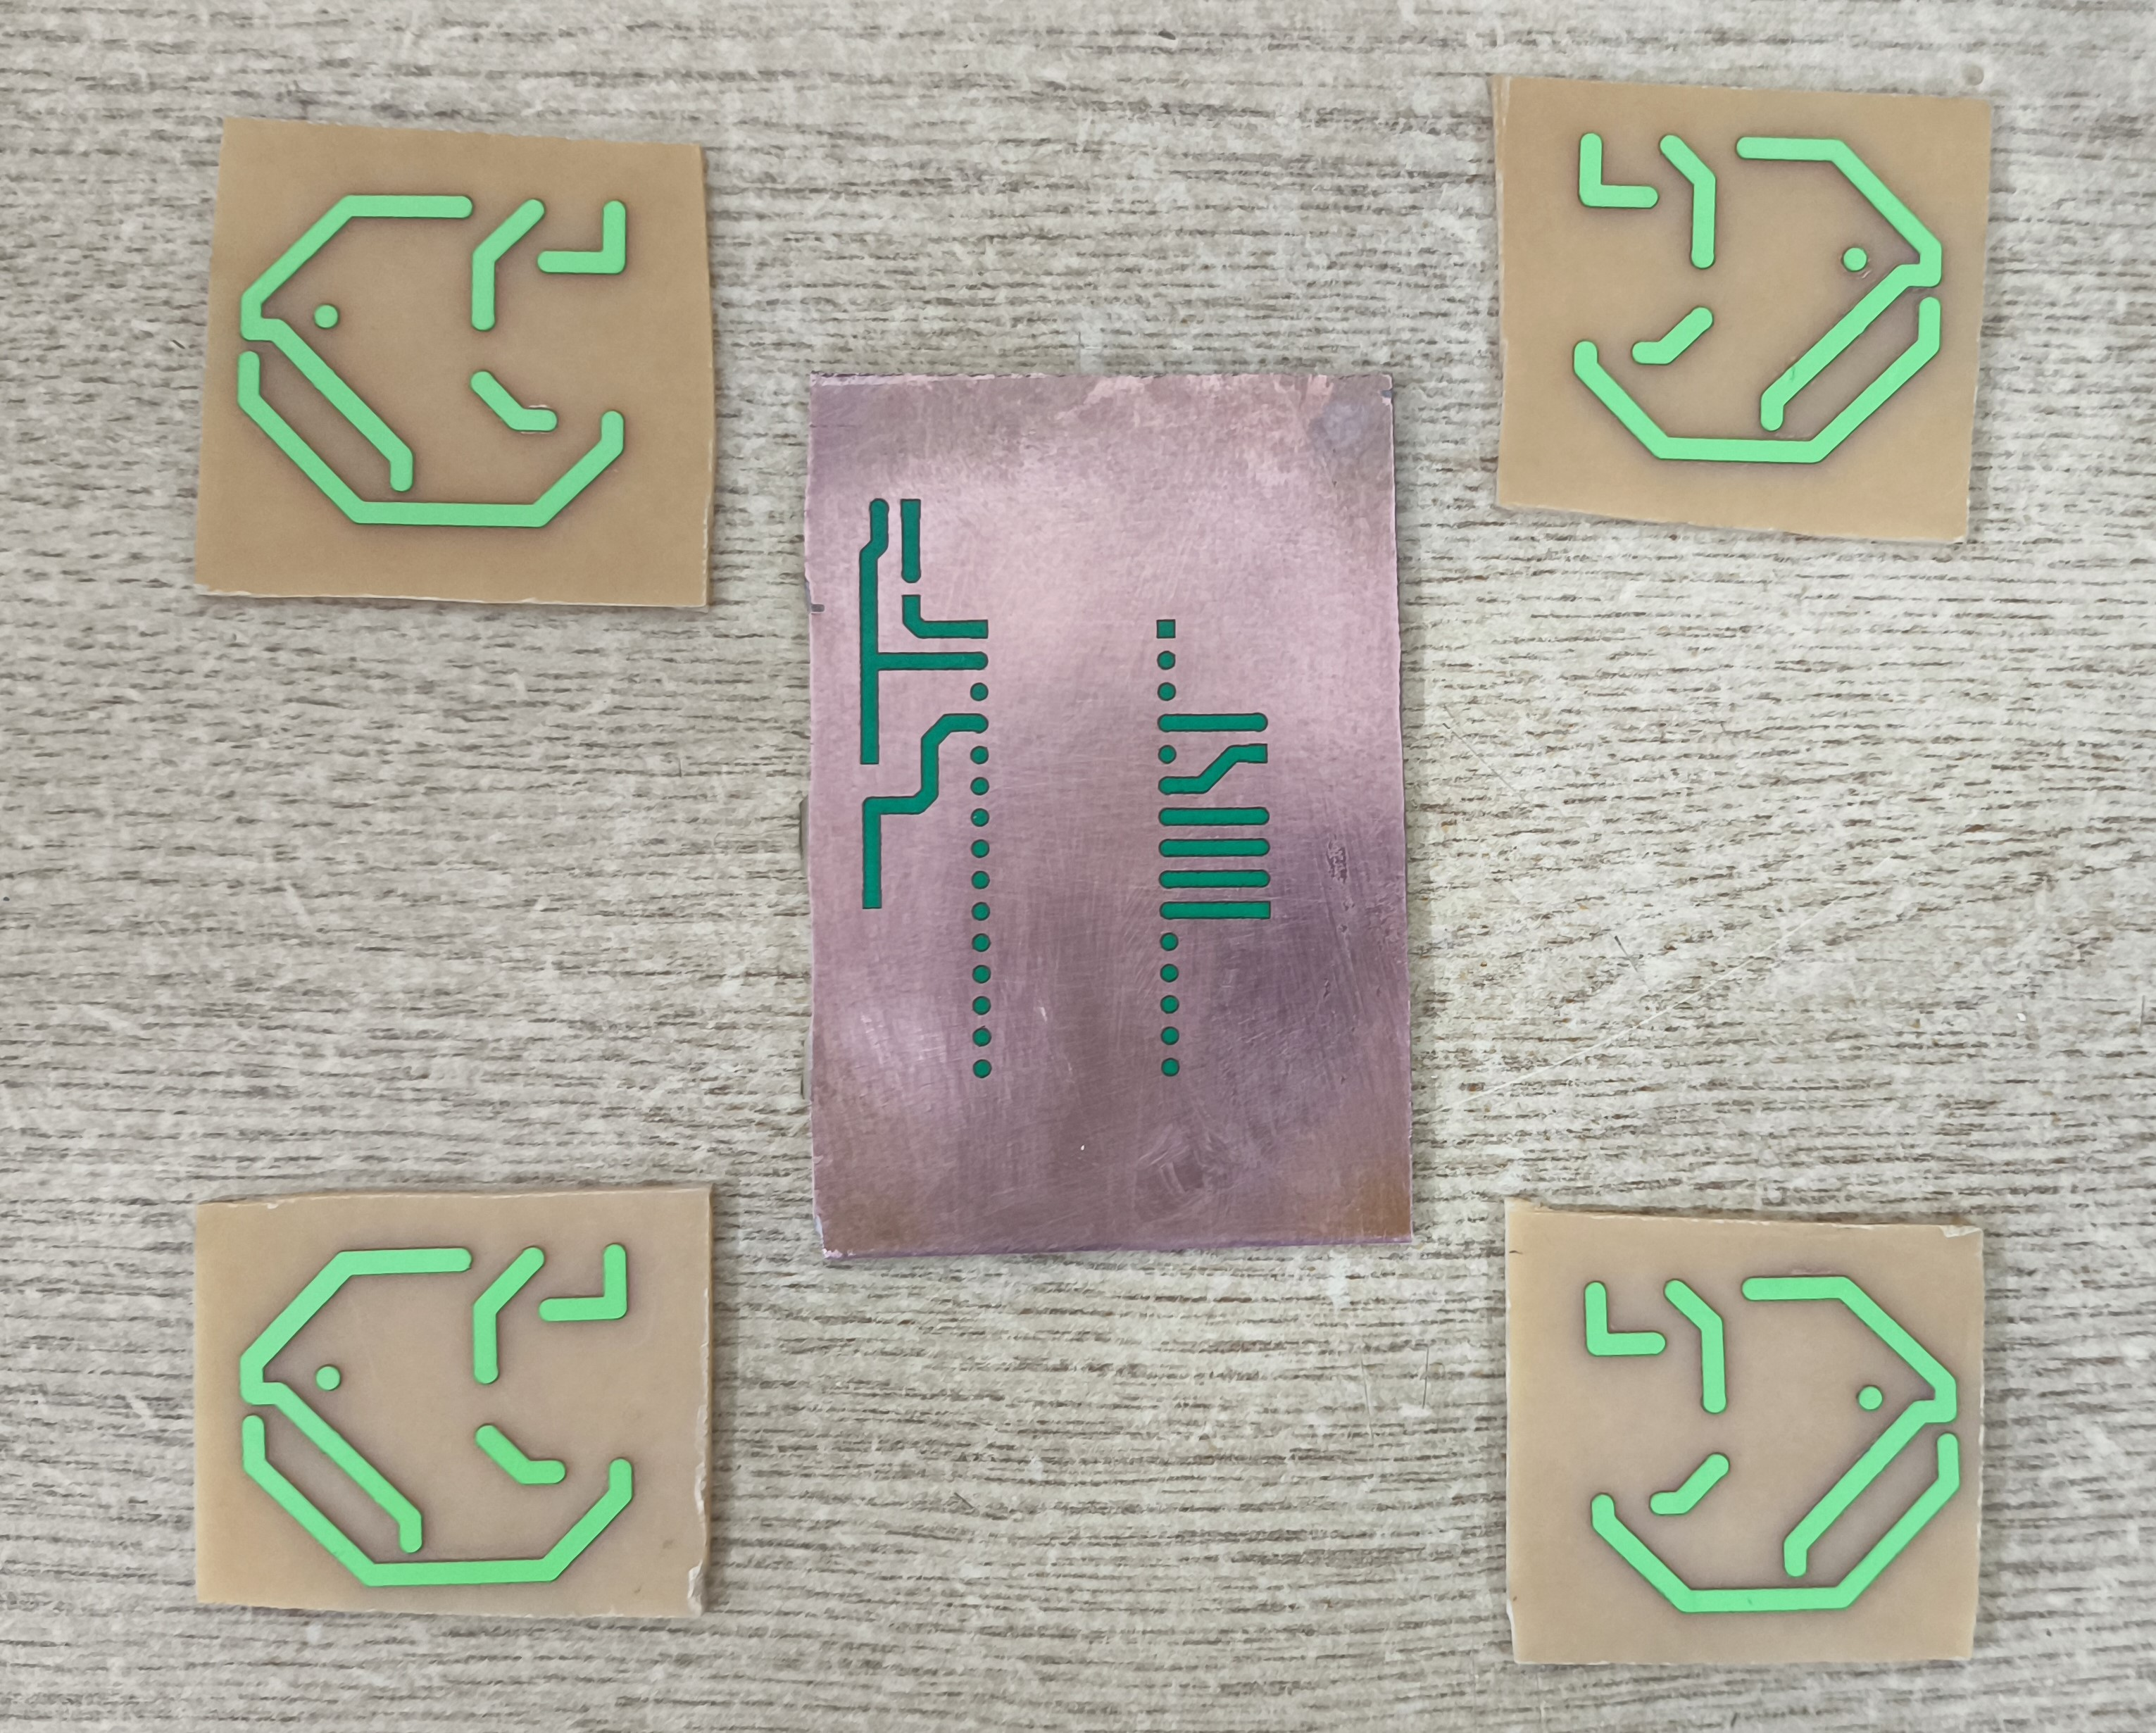
\includegraphics[width=0.4\textwidth,height=\textheight]{D:/Minha pasta/Estudos/UFPA/8º Semestre - 2024.2/Tópico Especiais em Eletrônica/Aluno/Ryan TEE/26.jpg}

Fig 27: Circuitos impresso.

A próxima etapa foi pegar as placas e fazer os furos de maneira manual aonde vão ficar os componentes, que nesse caso foi utilizado o furador do laboratório próprio para isso, na imagem a seguir temos as placas já furadas.

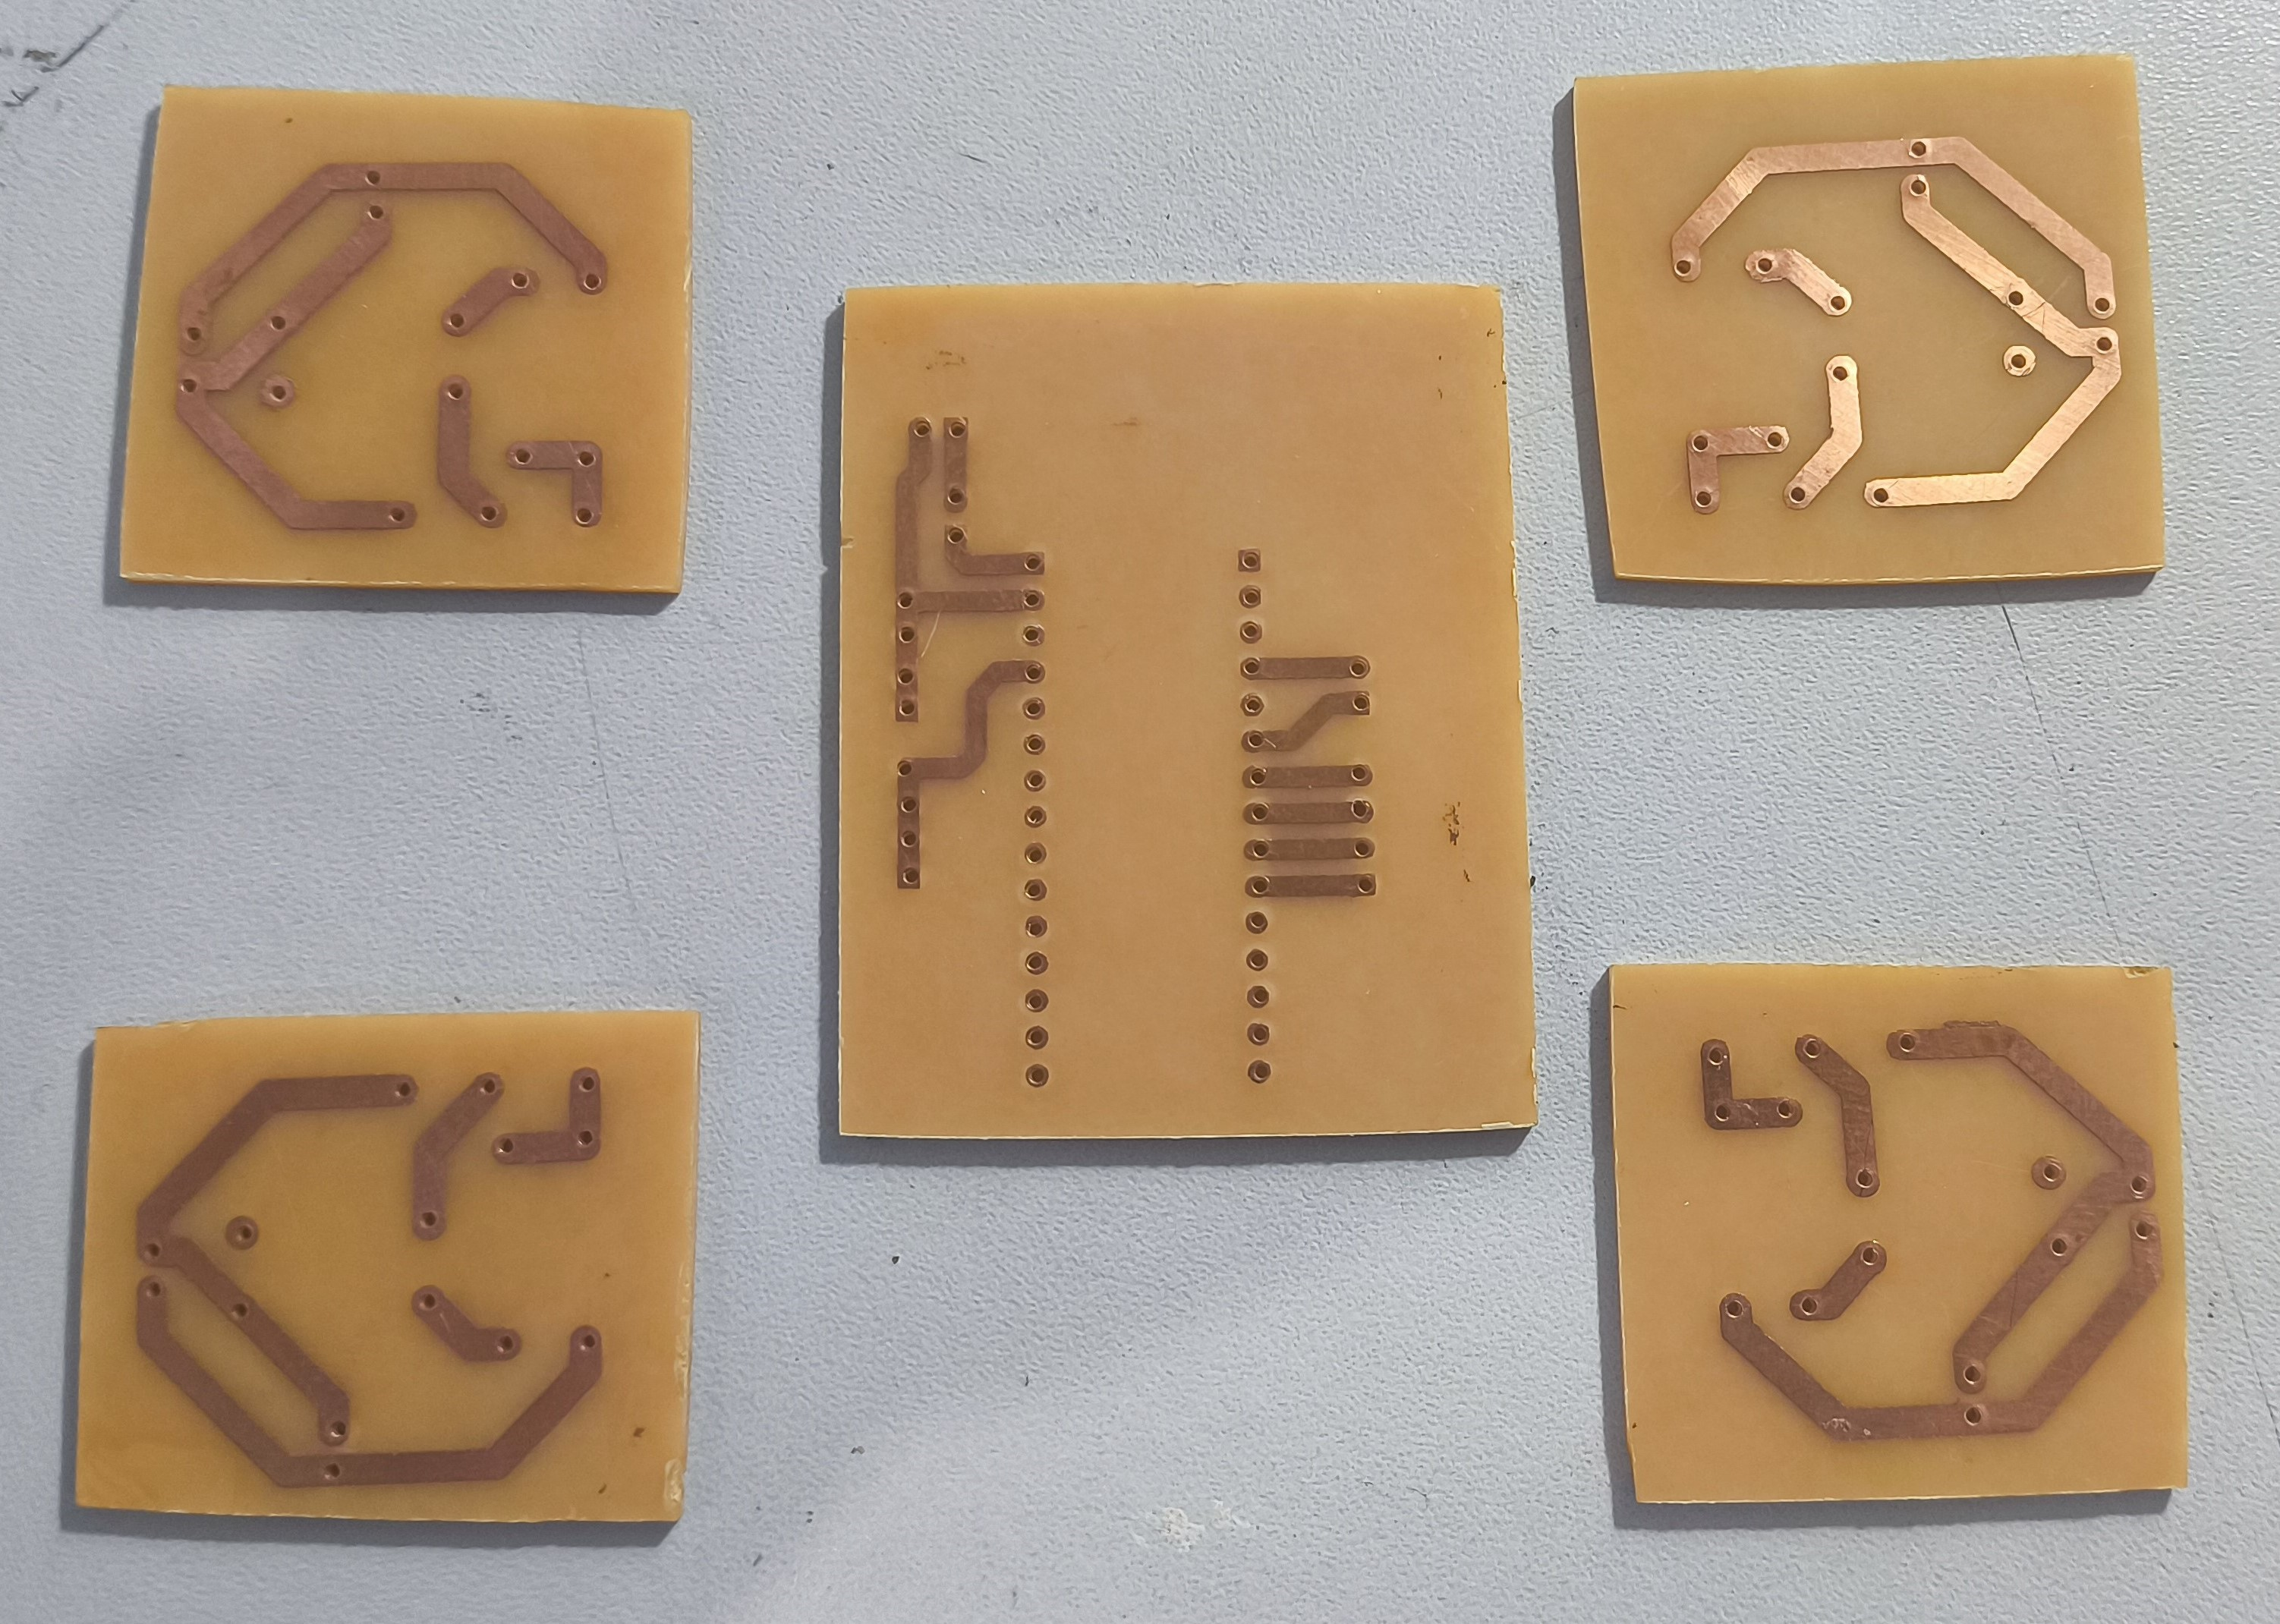
\includegraphics[width=0.4\textwidth,height=\textheight]{D:/Minha pasta/Estudos/UFPA/8º Semestre - 2024.2/Tópico Especiais em Eletrônica/Aluno/Ryan TEE/27.jpg}

Fig 28: PCBs furadas.

\section{Montagem e Soldagem da PCB:}\label{montagem-e-soldagem-da-pcb}

Soldar os componentes eletrônicos foi a próxima etapa. Realizei testes de continuidade para detectar possíveis erros, como mau contato. Na imagem, estou mostrando o processo de soldagem dos componentes e as cinco placas já finalizadas.

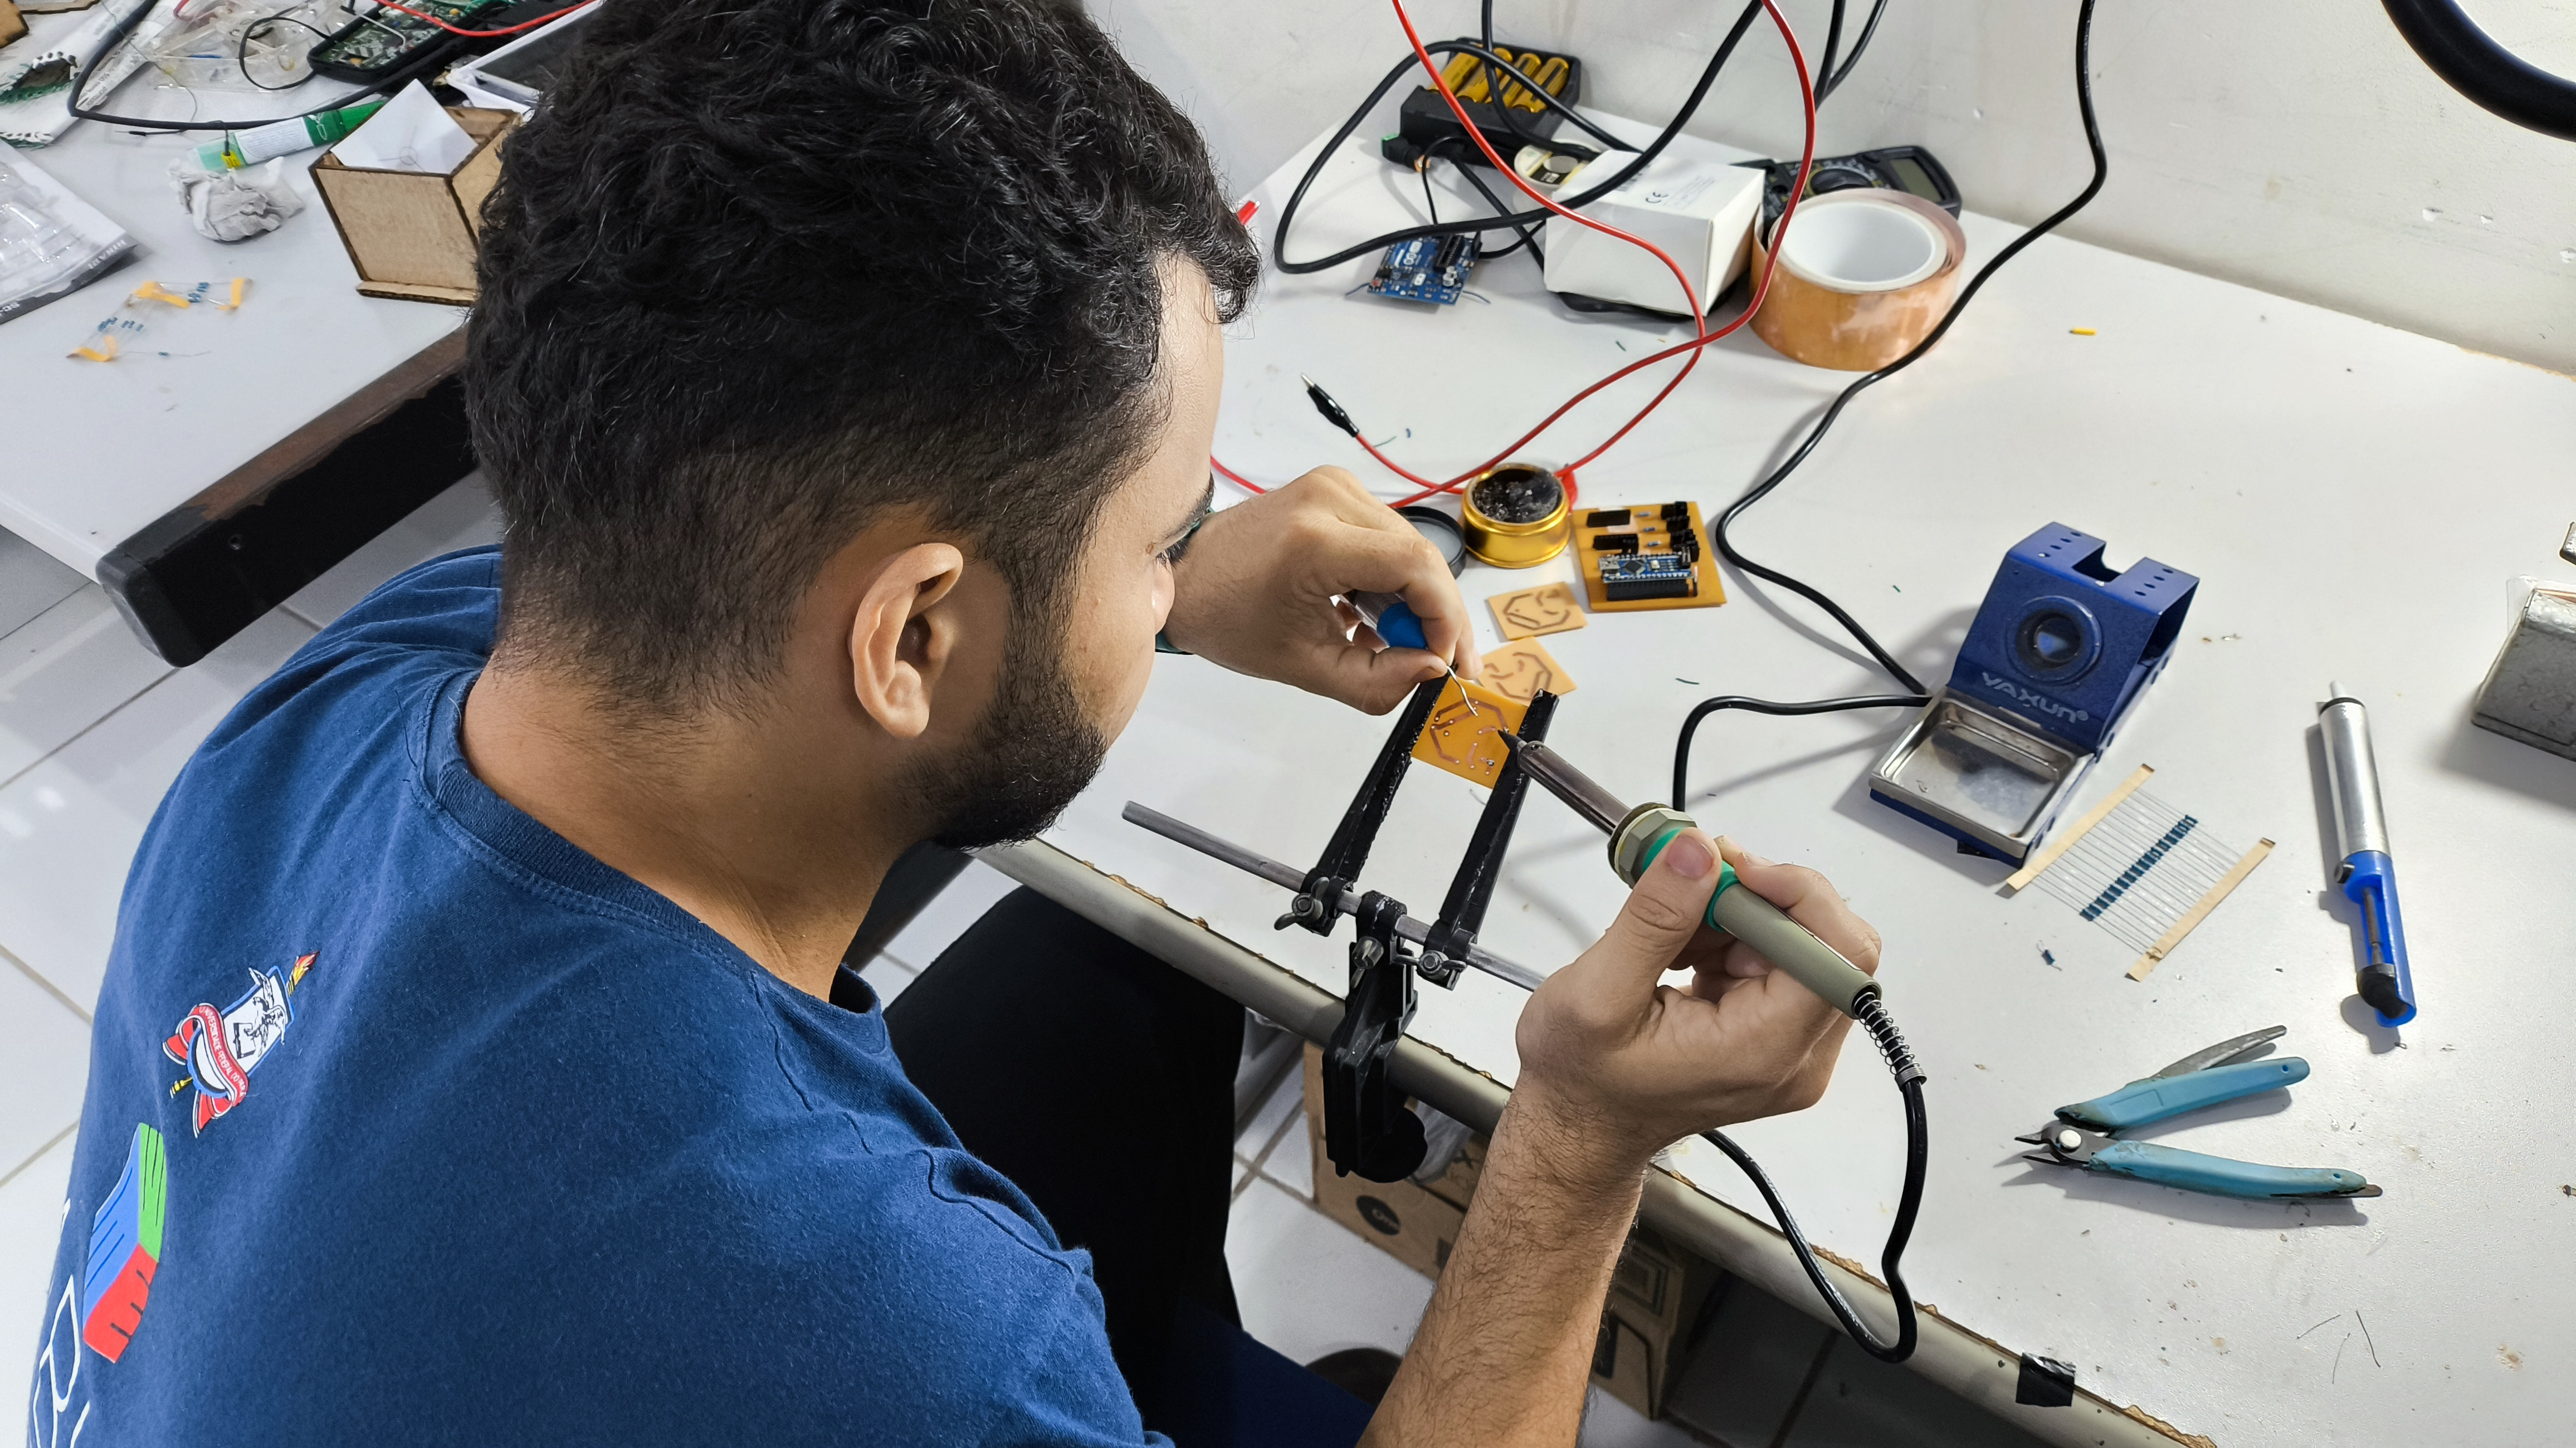
\includegraphics[width=0.55\textwidth,height=\textheight]{D:/Minha pasta/Estudos/UFPA/8º Semestre - 2024.2/Tópico Especiais em Eletrônica/Aluno/Ryan TEE/28.jpg}

Fig 29: Soldado os componentes.

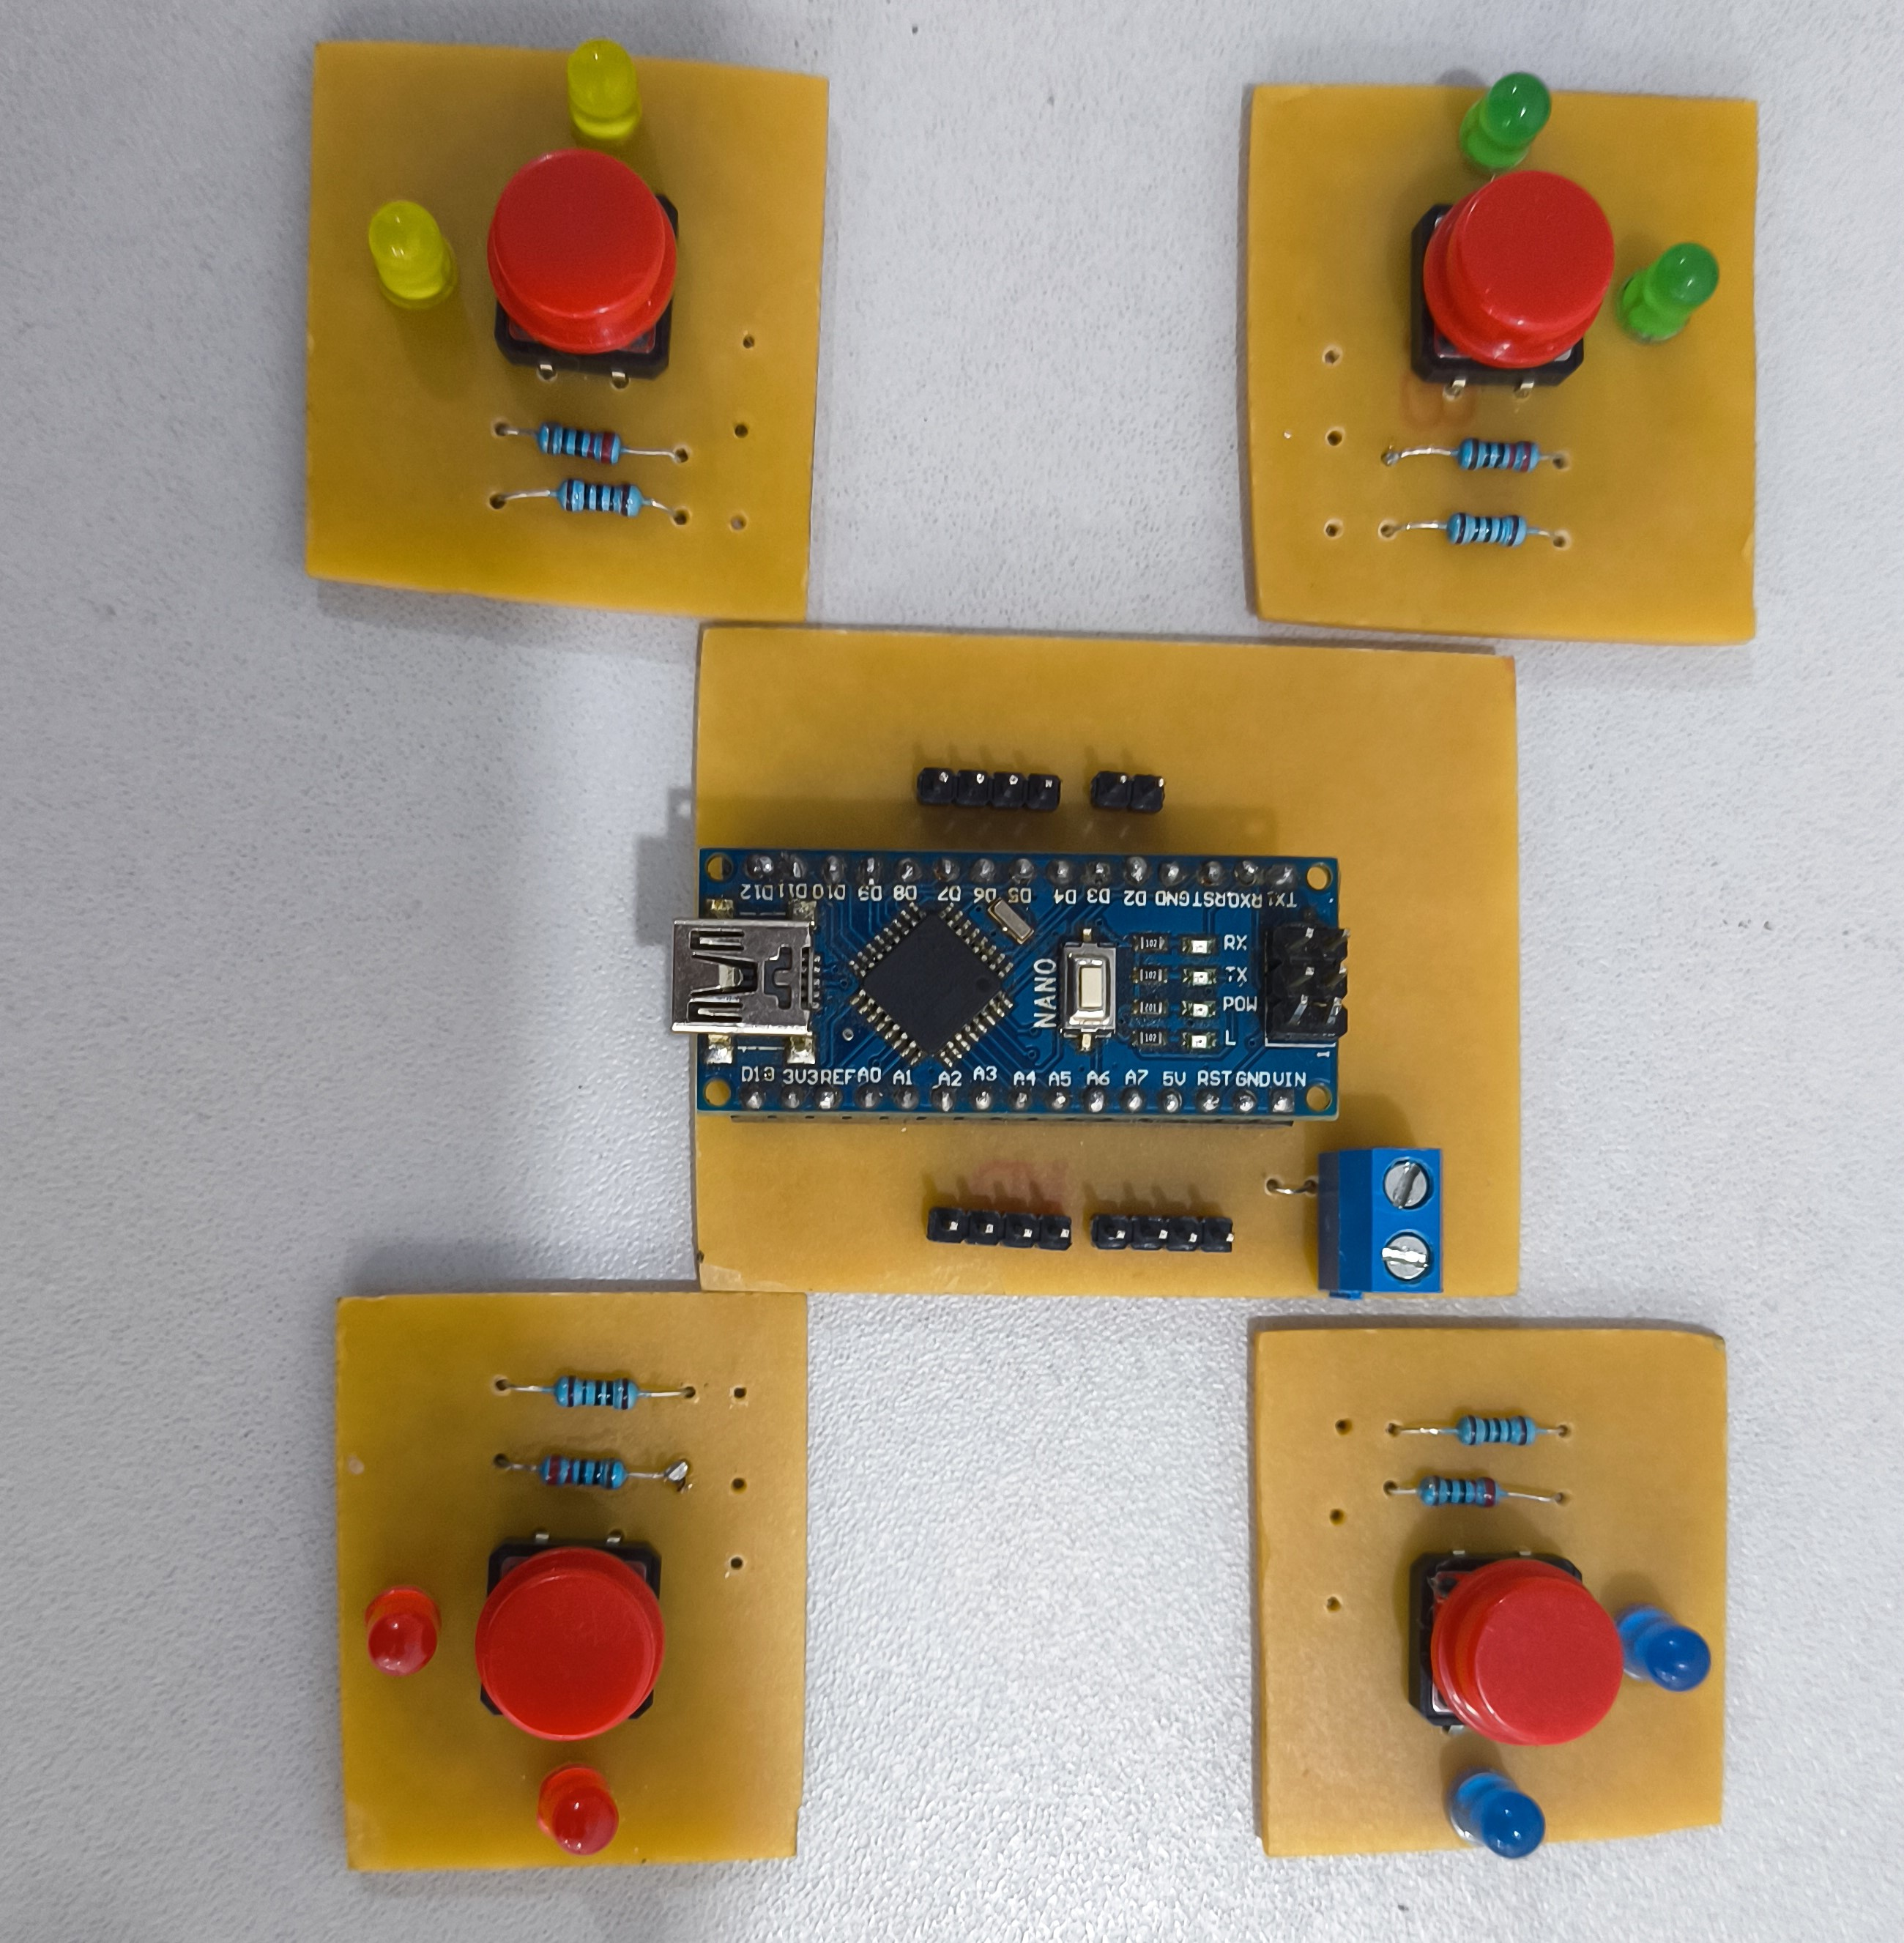
\includegraphics[width=0.4\textwidth,height=\textheight]{D:/Minha pasta/Estudos/UFPA/8º Semestre - 2024.2/Tópico Especiais em Eletrônica/Aluno/Ryan TEE/29.jpg}

Fig 30: Circuito montado.

Em seguida, conectei as cinco placas entre si e à placa principal, que é alimentada por uma bateria de 9 volts e possui uma chave liga/desliga. Testei todas as conexões e ajustei o código conforme necessário, garantindo que tudo funcionasse perfeitamente.

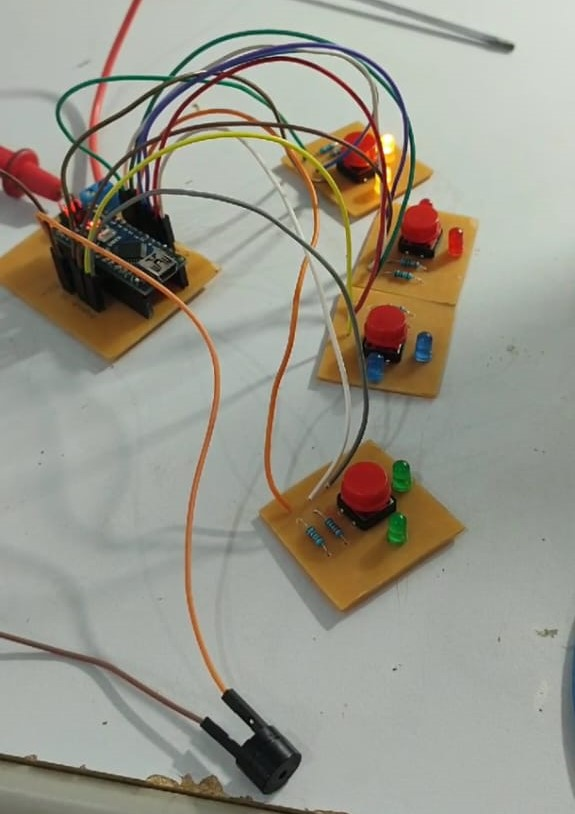
\includegraphics[width=0.37\textwidth,height=\textheight]{D:/Minha pasta/Estudos/UFPA/8º Semestre - 2024.2/Tópico Especiais em Eletrônica/Aluno/Ryan TEE/30.jpeg}

Fig 31: Teste das placas.

\section{Design da Caixa:}\label{design-da-caixa}

Após garantir que o sistema elétrico e o código estavam funcionando perfeitamente, o foco seguinte foi desenvolver a parte mecânica e estética do projeto. Para começar, utilizei o MakerCase para criar a caixa nas dimensões desejadas. Em seguida, fiz ajustes estéticos, como a inclusão do logo e nome do FABLAB, além do nome GENIUS. Também foram feitas modificações mecânicas essenciais, como a criação do espaço para as teclas dos botões, a abertura para a chave liga-desliga, o posicionamento para a saída do buzzer e uma entrada para o Arduino, possibilitando futuras melhorias ou correções no código. Optei por construir a caixa em MDF. Na imagem abaixo, é possível visualizar o arquivo que gerou o modelo da caixa.

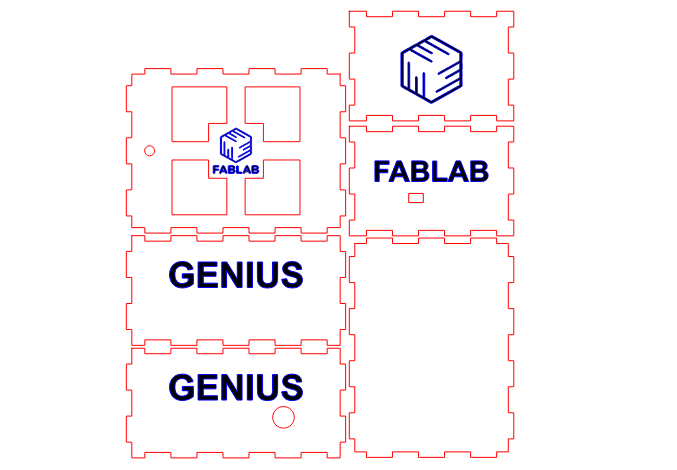
\includegraphics[width=0.6\textwidth,height=\textheight]{D:/Minha pasta/Estudos/UFPA/8º Semestre - 2024.2/Tópico Especiais em Eletrônica/Aluno/Ryan TEE/31.png}

Fig 32: Desenho da caixa.

Com a estrutura da caixa finalizada, o próximo desafio foi projetar as teclas para pressionar os botões. Decidi utilizar teclas de acrílico para permitir a visualização das luzes emitidas pelos LEDs. Para garantir que os botões ficassem suspensos de maneira adequada, desenvolvi uma base que mantém os botões na posição correta, como mostrado na imagem a seguir.

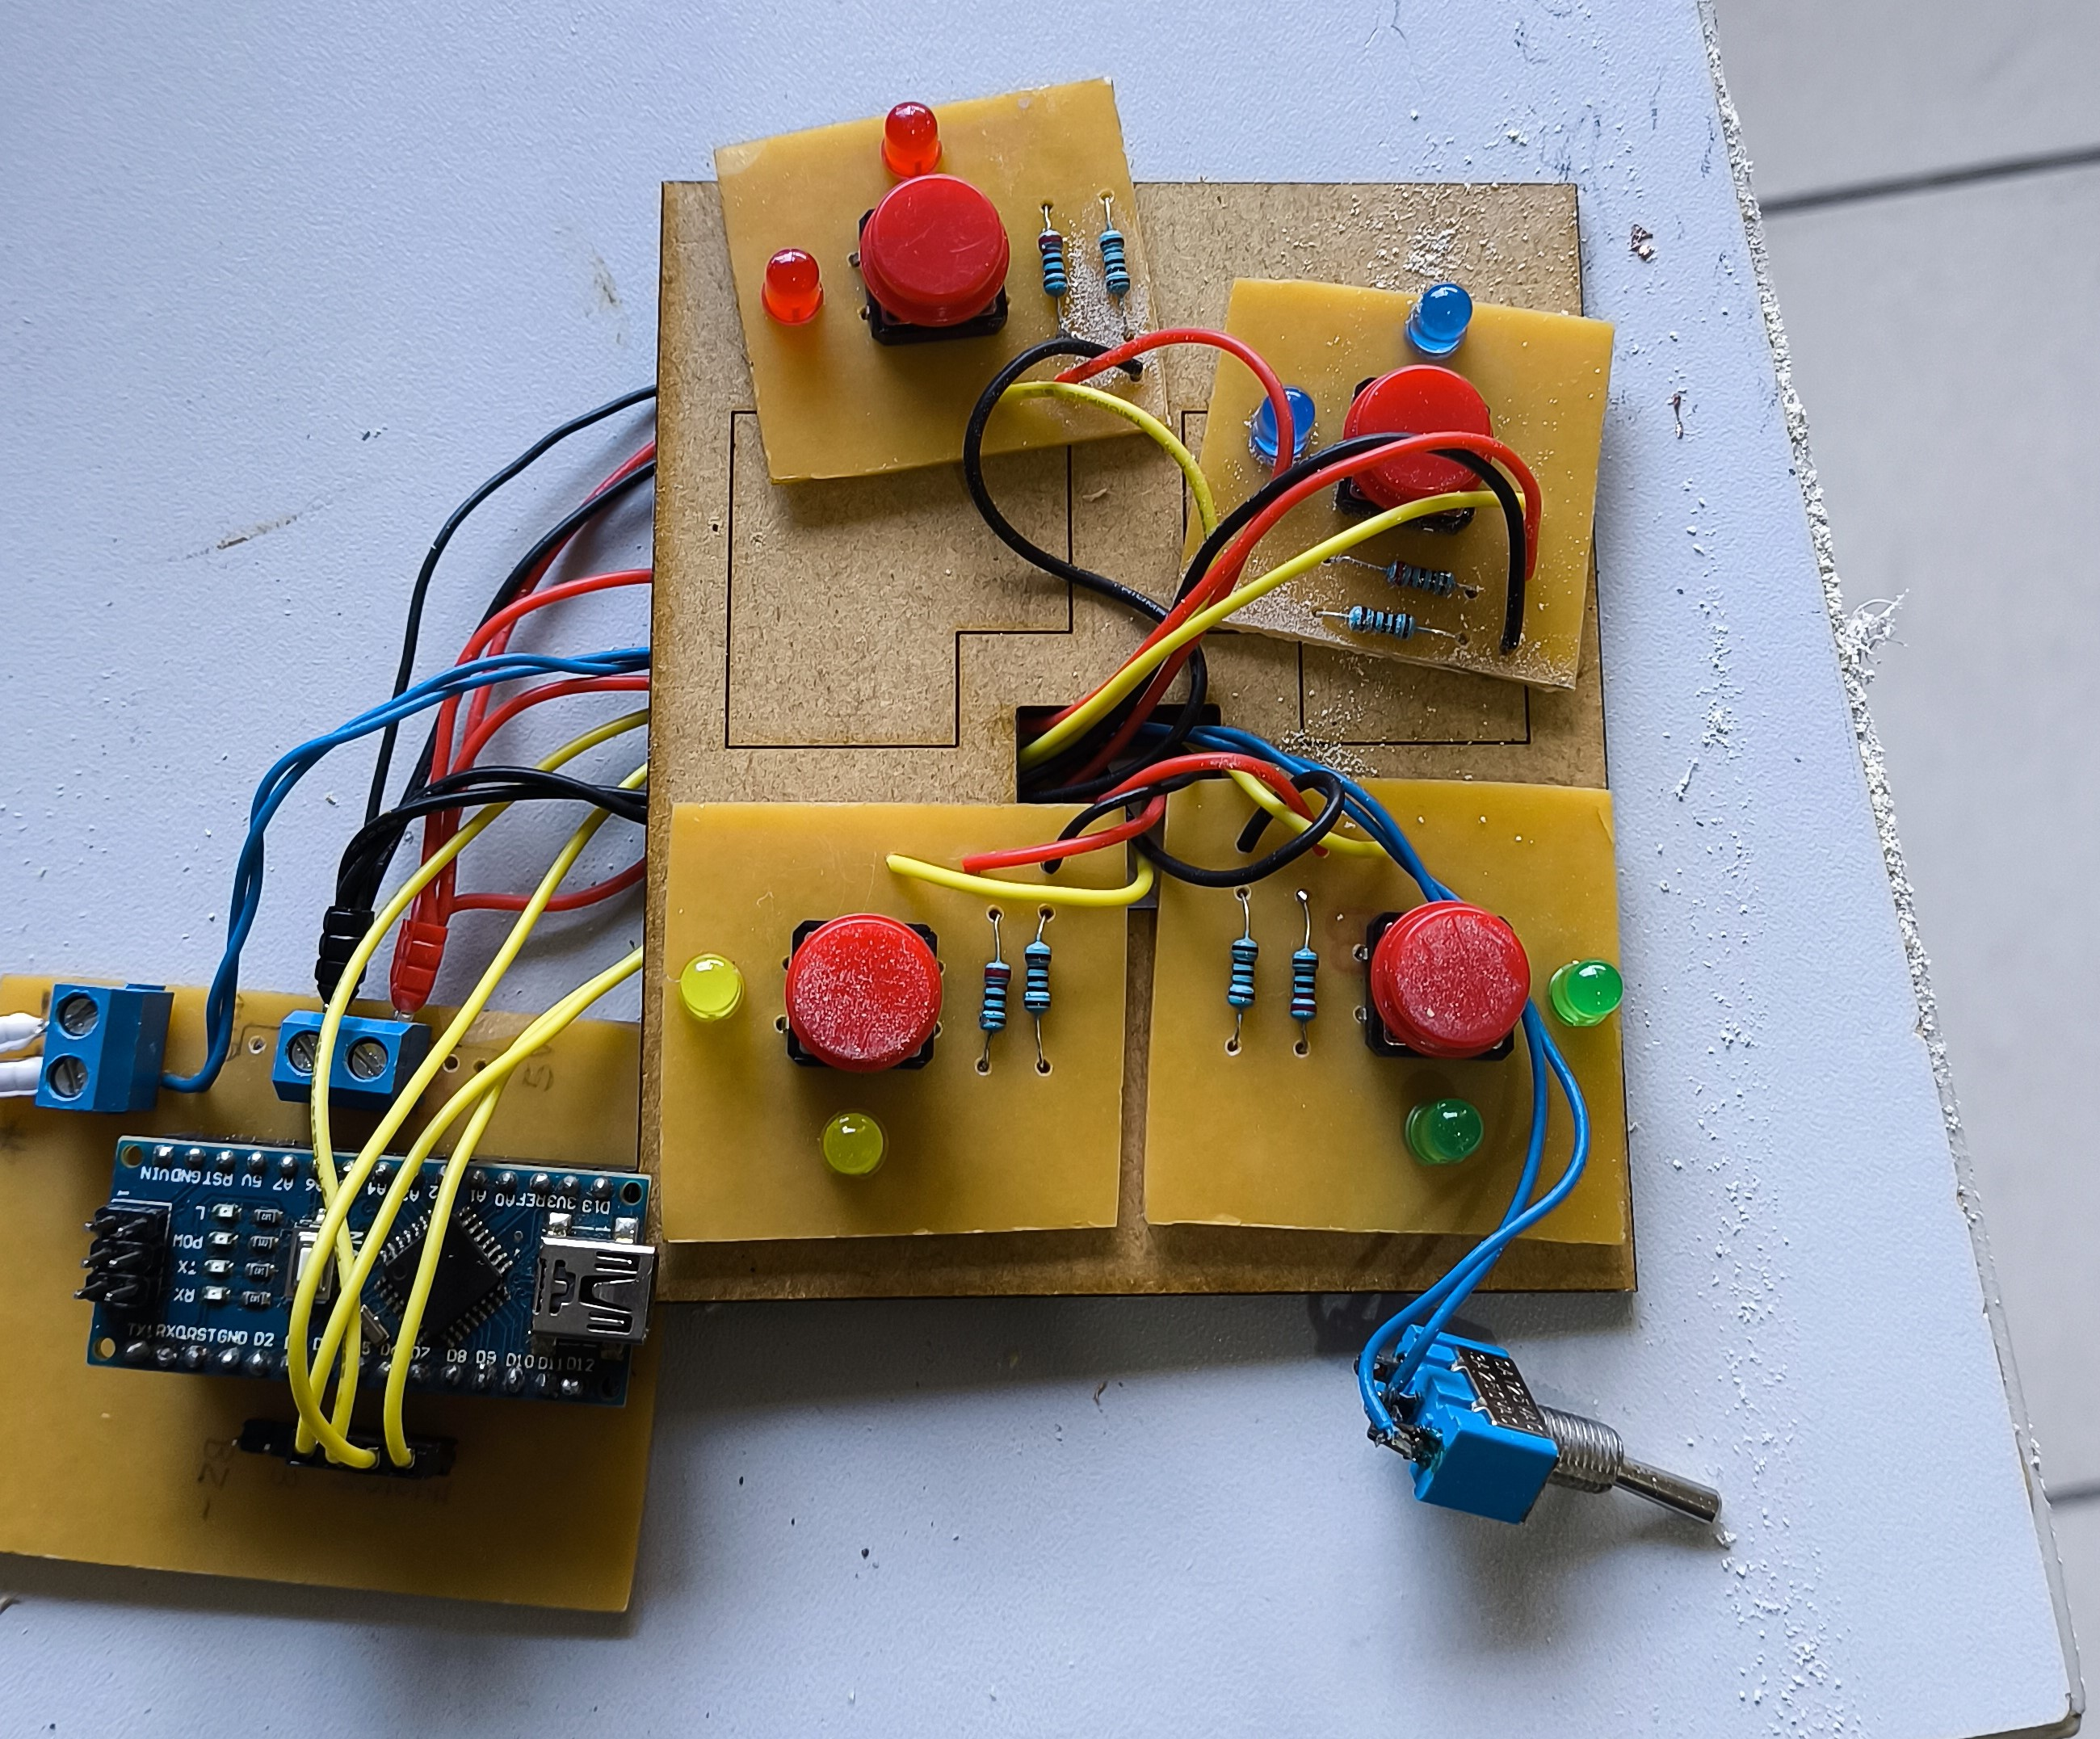
\includegraphics[width=0.4\textwidth,height=\textheight]{D:/Minha pasta/Estudos/UFPA/8º Semestre - 2024.2/Tópico Especiais em Eletrônica/Aluno/Ryan TEE/32.jpg}

Fig 33: Base para os botões.

Para manter as teclas no lugar, foi necessário cria um sistema na tampa da caixa, que as teclas ficariam entre duas peças, onde ela se movimentaria, mas sem sair do lugar, na imagem a segui temos o desenho que foi feito essa peça, sendo a parte de dentro a menor é a parte de baixo, e parte maior é a parte de cima.

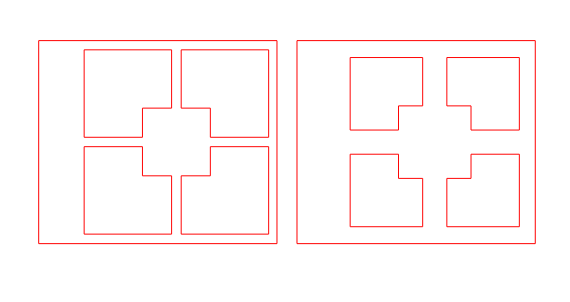
\includegraphics[width=0.6\textwidth,height=\textheight]{D:/Minha pasta/Estudos/UFPA/8º Semestre - 2024.2/Tópico Especiais em Eletrônica/Aluno/Ryan TEE/33.png}

Fig 34: Tampa para as teclas.

\section{Montagem Final:}\label{montagem-final}

Com todos os detalhes resolvidos, chegou o momento de montar a caixa de fato. Na estrutura vazia da caixa, foram adicionados apoios nos cantos para segurar a base dos botões, como pode ser observado na imagem a seguir.

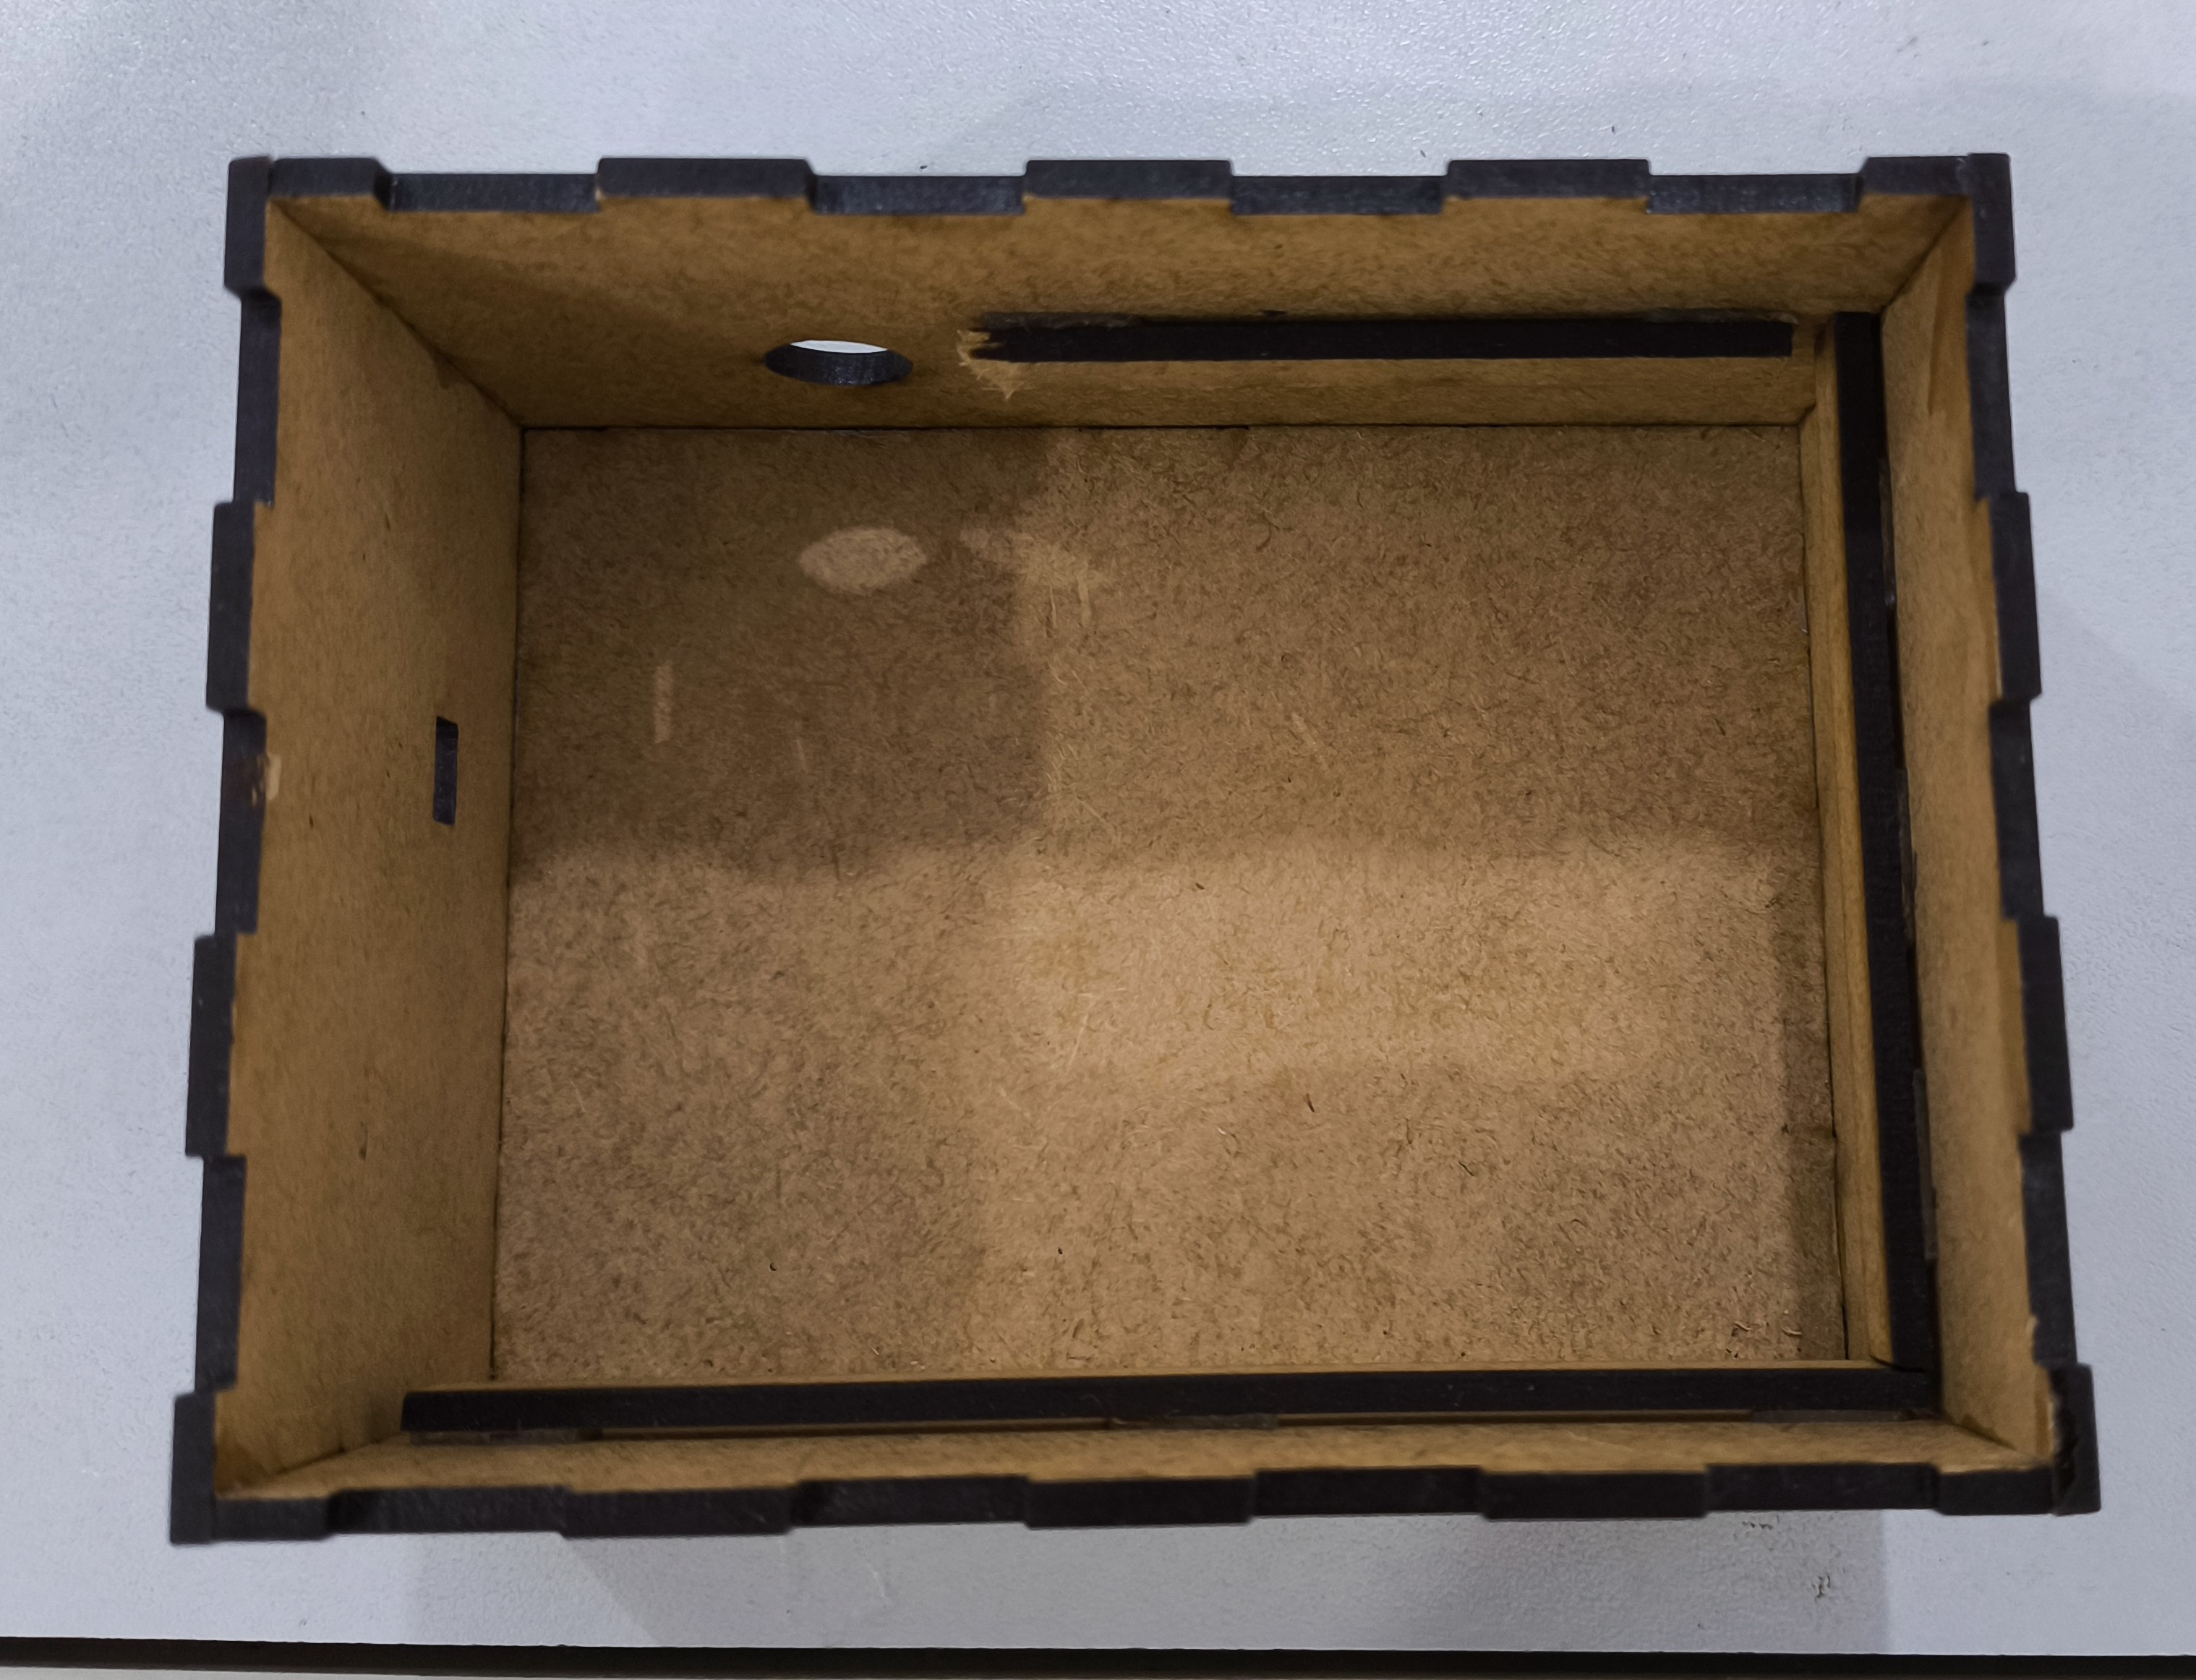
\includegraphics[width=0.5\textwidth,height=\textheight]{D:/Minha pasta/Estudos/UFPA/8º Semestre - 2024.2/Tópico Especiais em Eletrônica/Aluno/Ryan TEE/34.jpg}

Fig 35: Parte interna da caixa vazia.

Em seguida, a placa principal e a bateria foram instaladas na parte inferior da caixa, conforme mostrado na imagem a seguir.

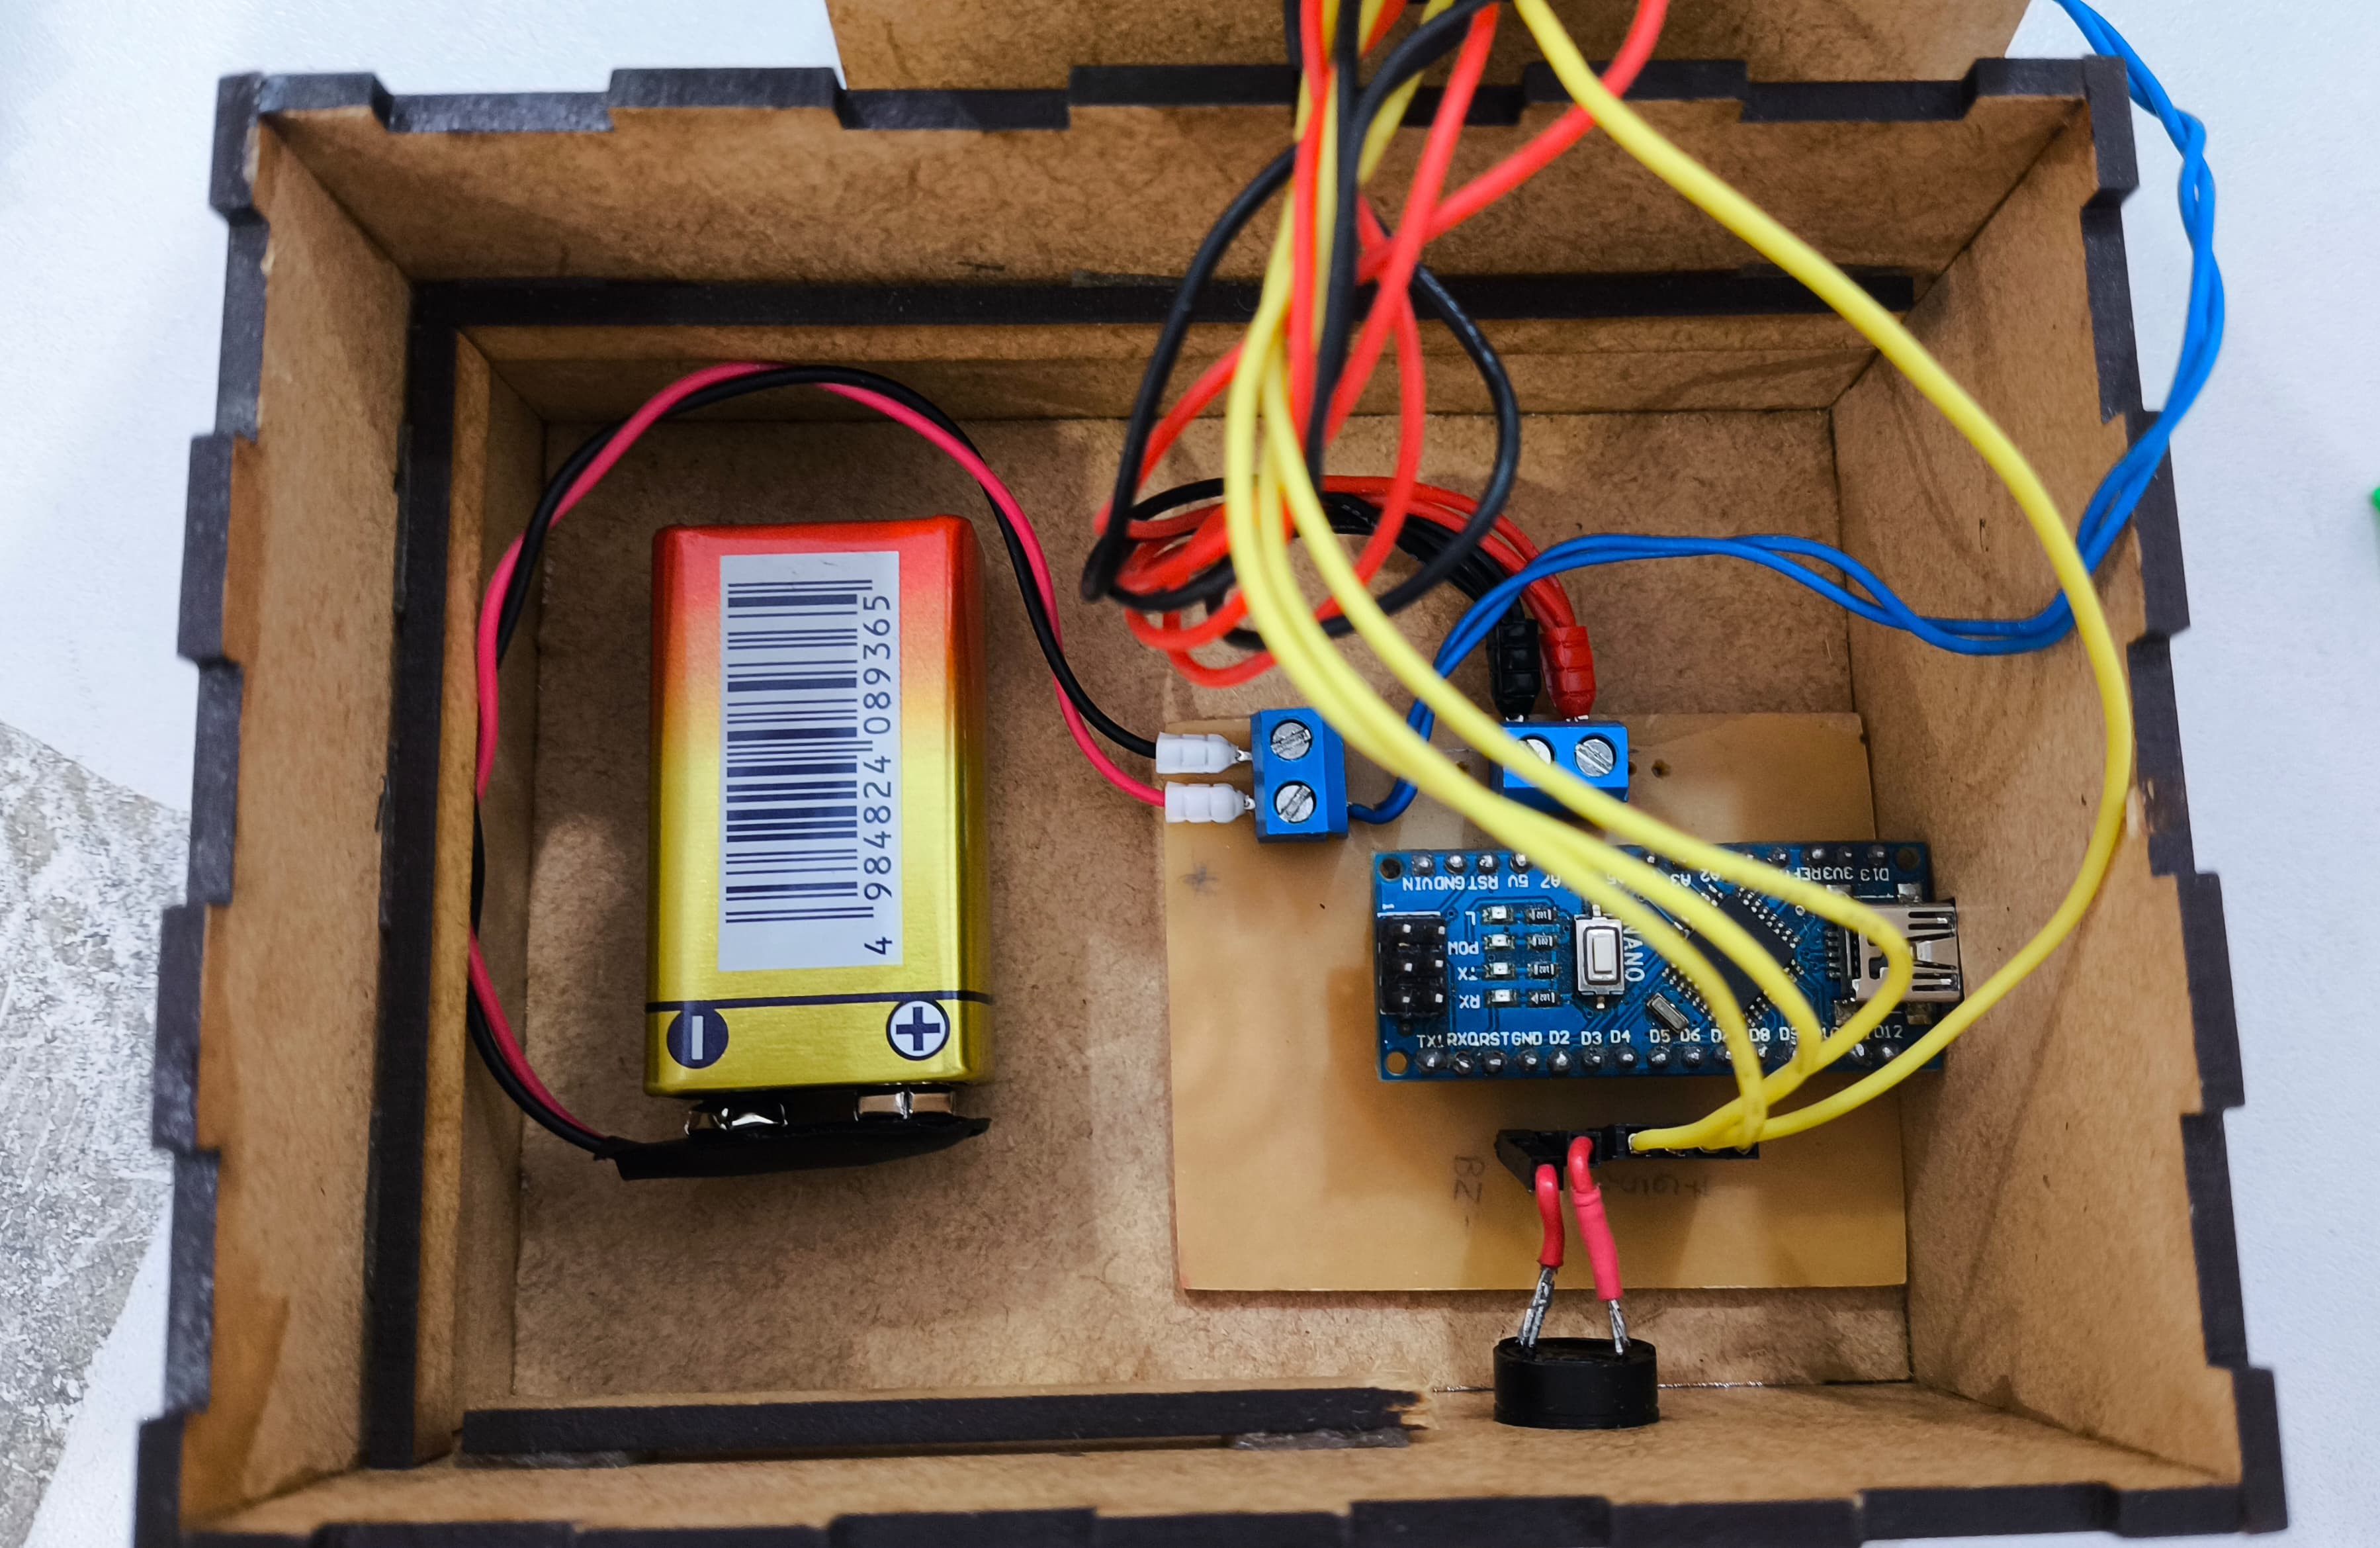
\includegraphics[width=0.5\textwidth,height=\textheight]{D:/Minha pasta/Estudos/UFPA/8º Semestre - 2024.2/Tópico Especiais em Eletrônica/Aluno/Ryan TEE/35.jpeg}

Fig 36: Parte interna da caixa com a placa principal e a bateria.

Posteriormente, os botões e os LEDs com suas bases foram posicionados sobre os suportes preparados, como mostrado na imagem.

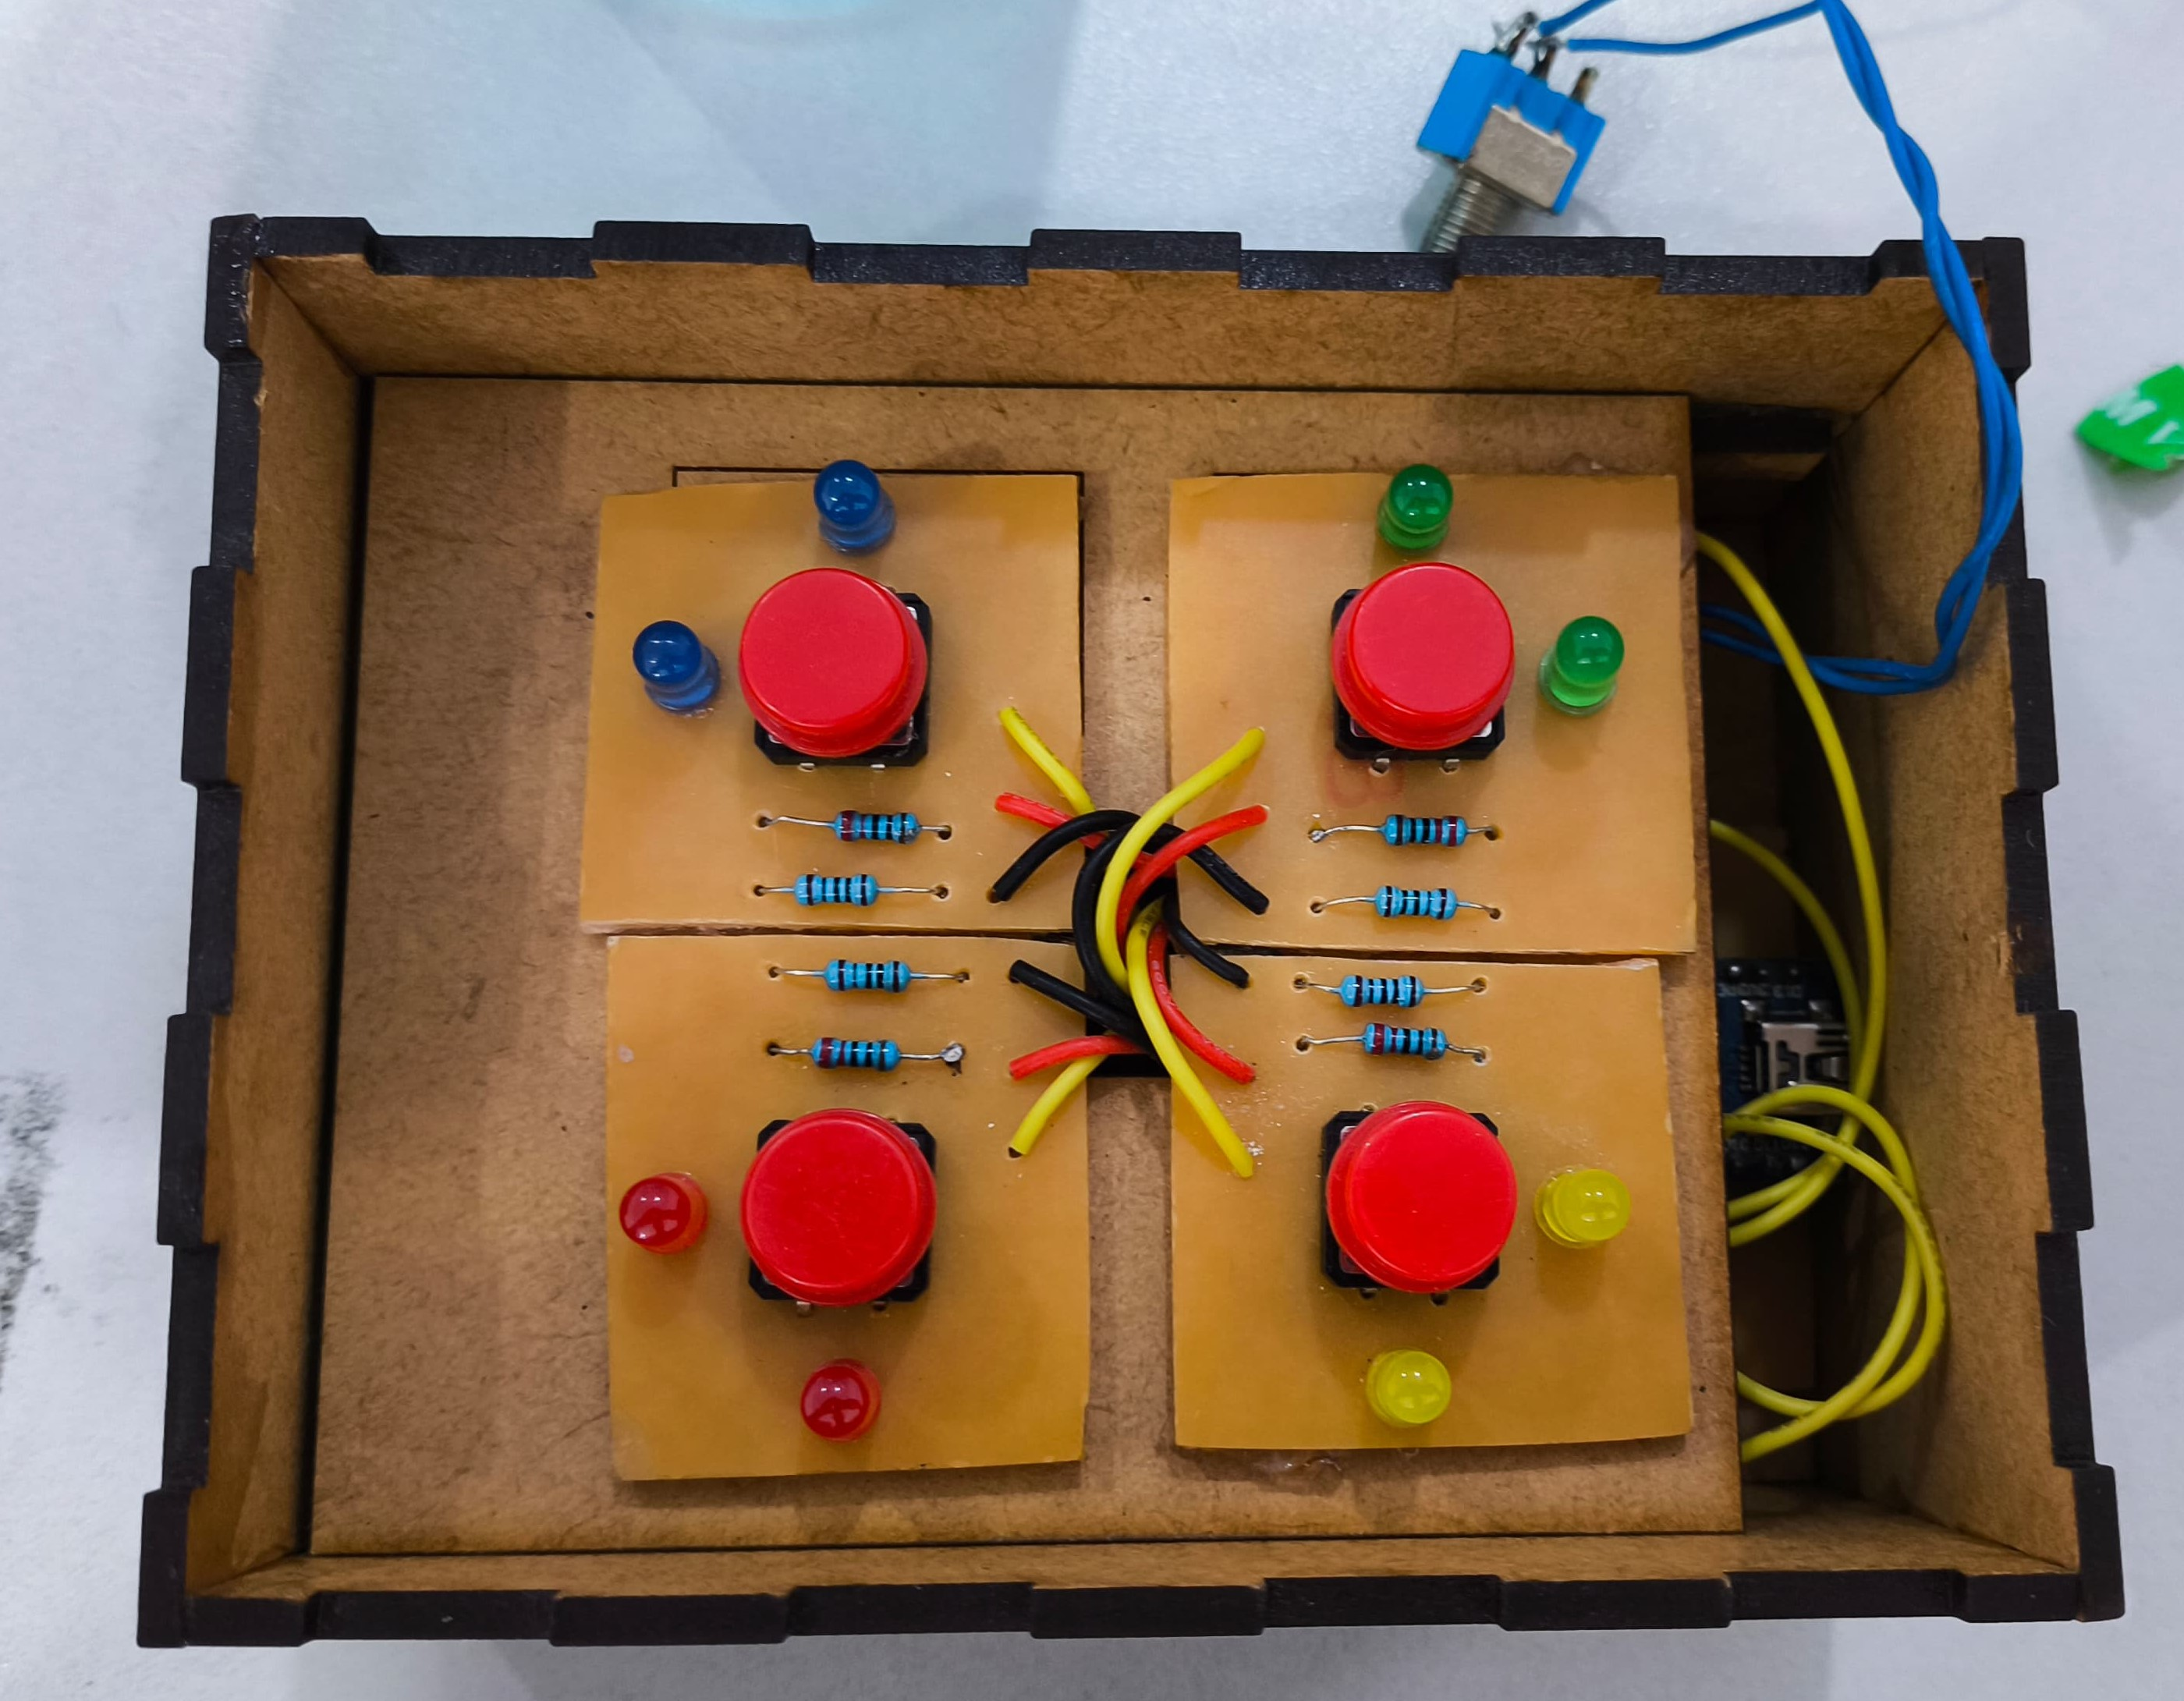
\includegraphics[width=0.5\textwidth,height=\textheight]{D:/Minha pasta/Estudos/UFPA/8º Semestre - 2024.2/Tópico Especiais em Eletrônica/Aluno/Ryan TEE/36.jpeg}

Fig 37: Parte interna da caixa com os botões.

Por fim, a tampa da caixa foi colocada, onde estão as teclas e a chave liga-desliga, como ilustrado na imagem final. Com todos os componentes montados, temos um jogo GENIUS funcional. A cada rodada, sequências aleatórias são apresentadas, proporcionando diversão ao usuário. A seguir, algumas imagens do produto final.

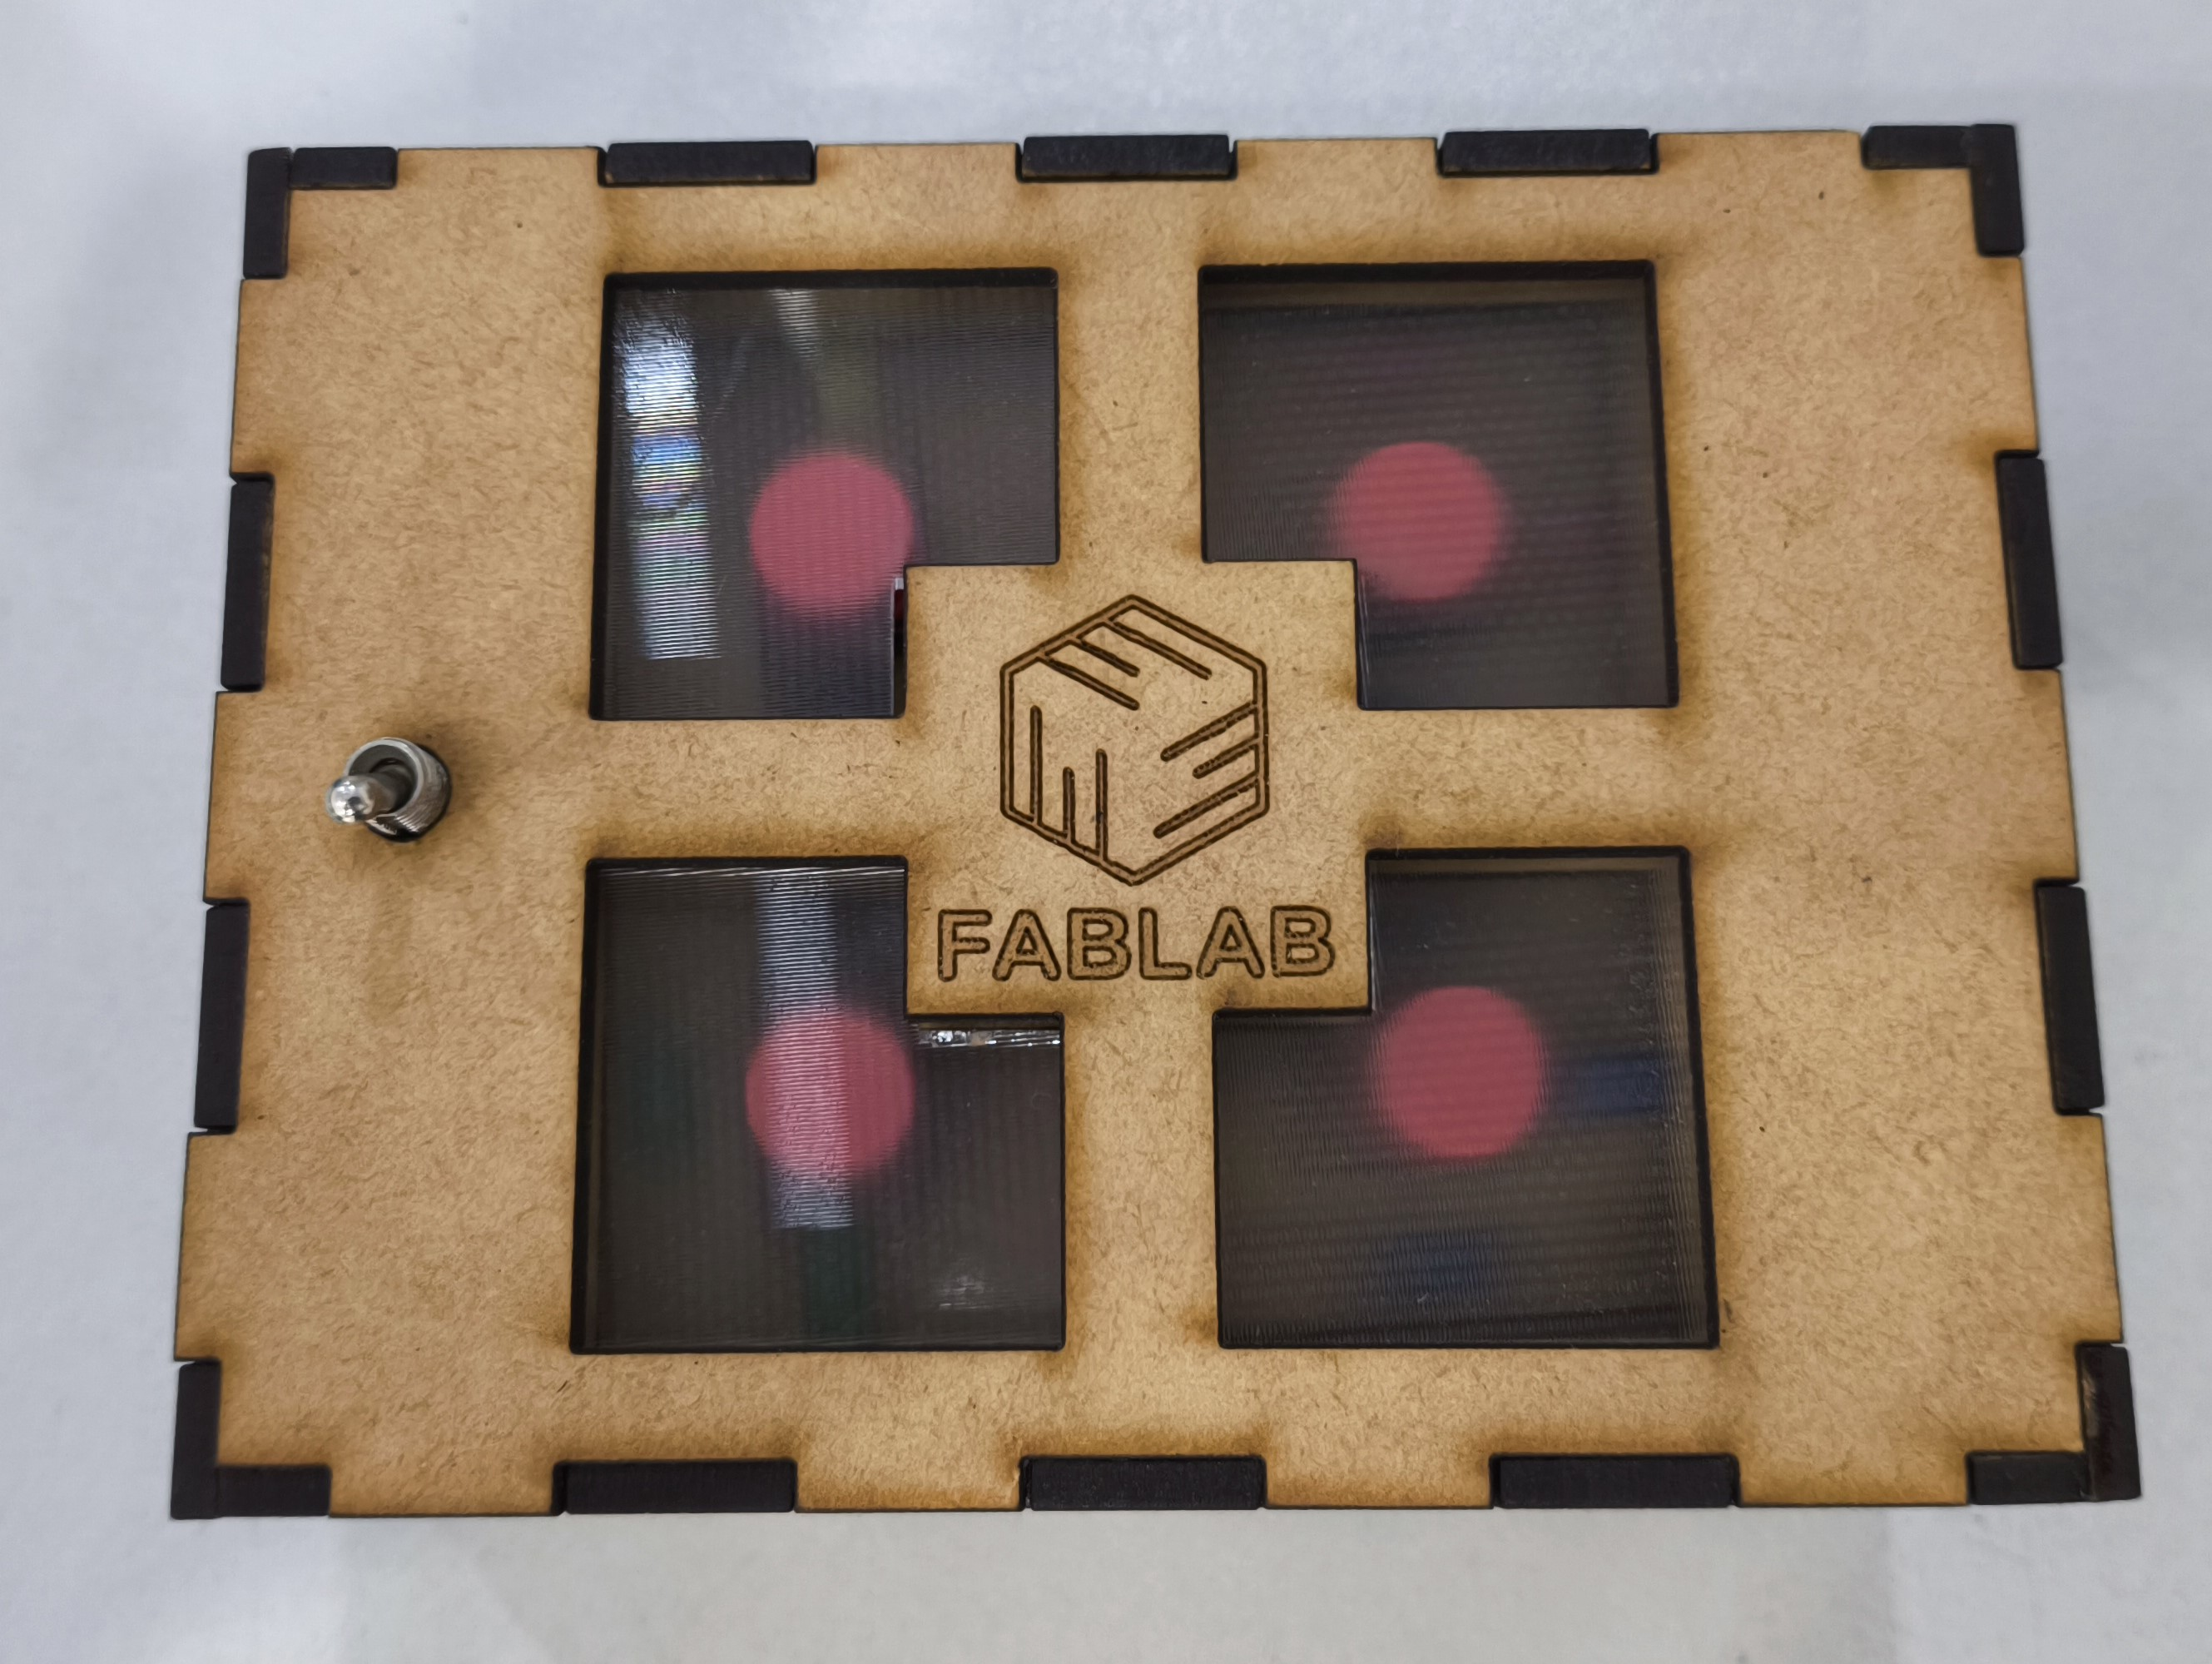
\includegraphics[width=0.5\textwidth,height=\textheight]{D:/Minha pasta/Estudos/UFPA/8º Semestre - 2024.2/Tópico Especiais em Eletrônica/Aluno/Ryan TEE/37.jpg}

Fig 38: Vista superior da caixa.

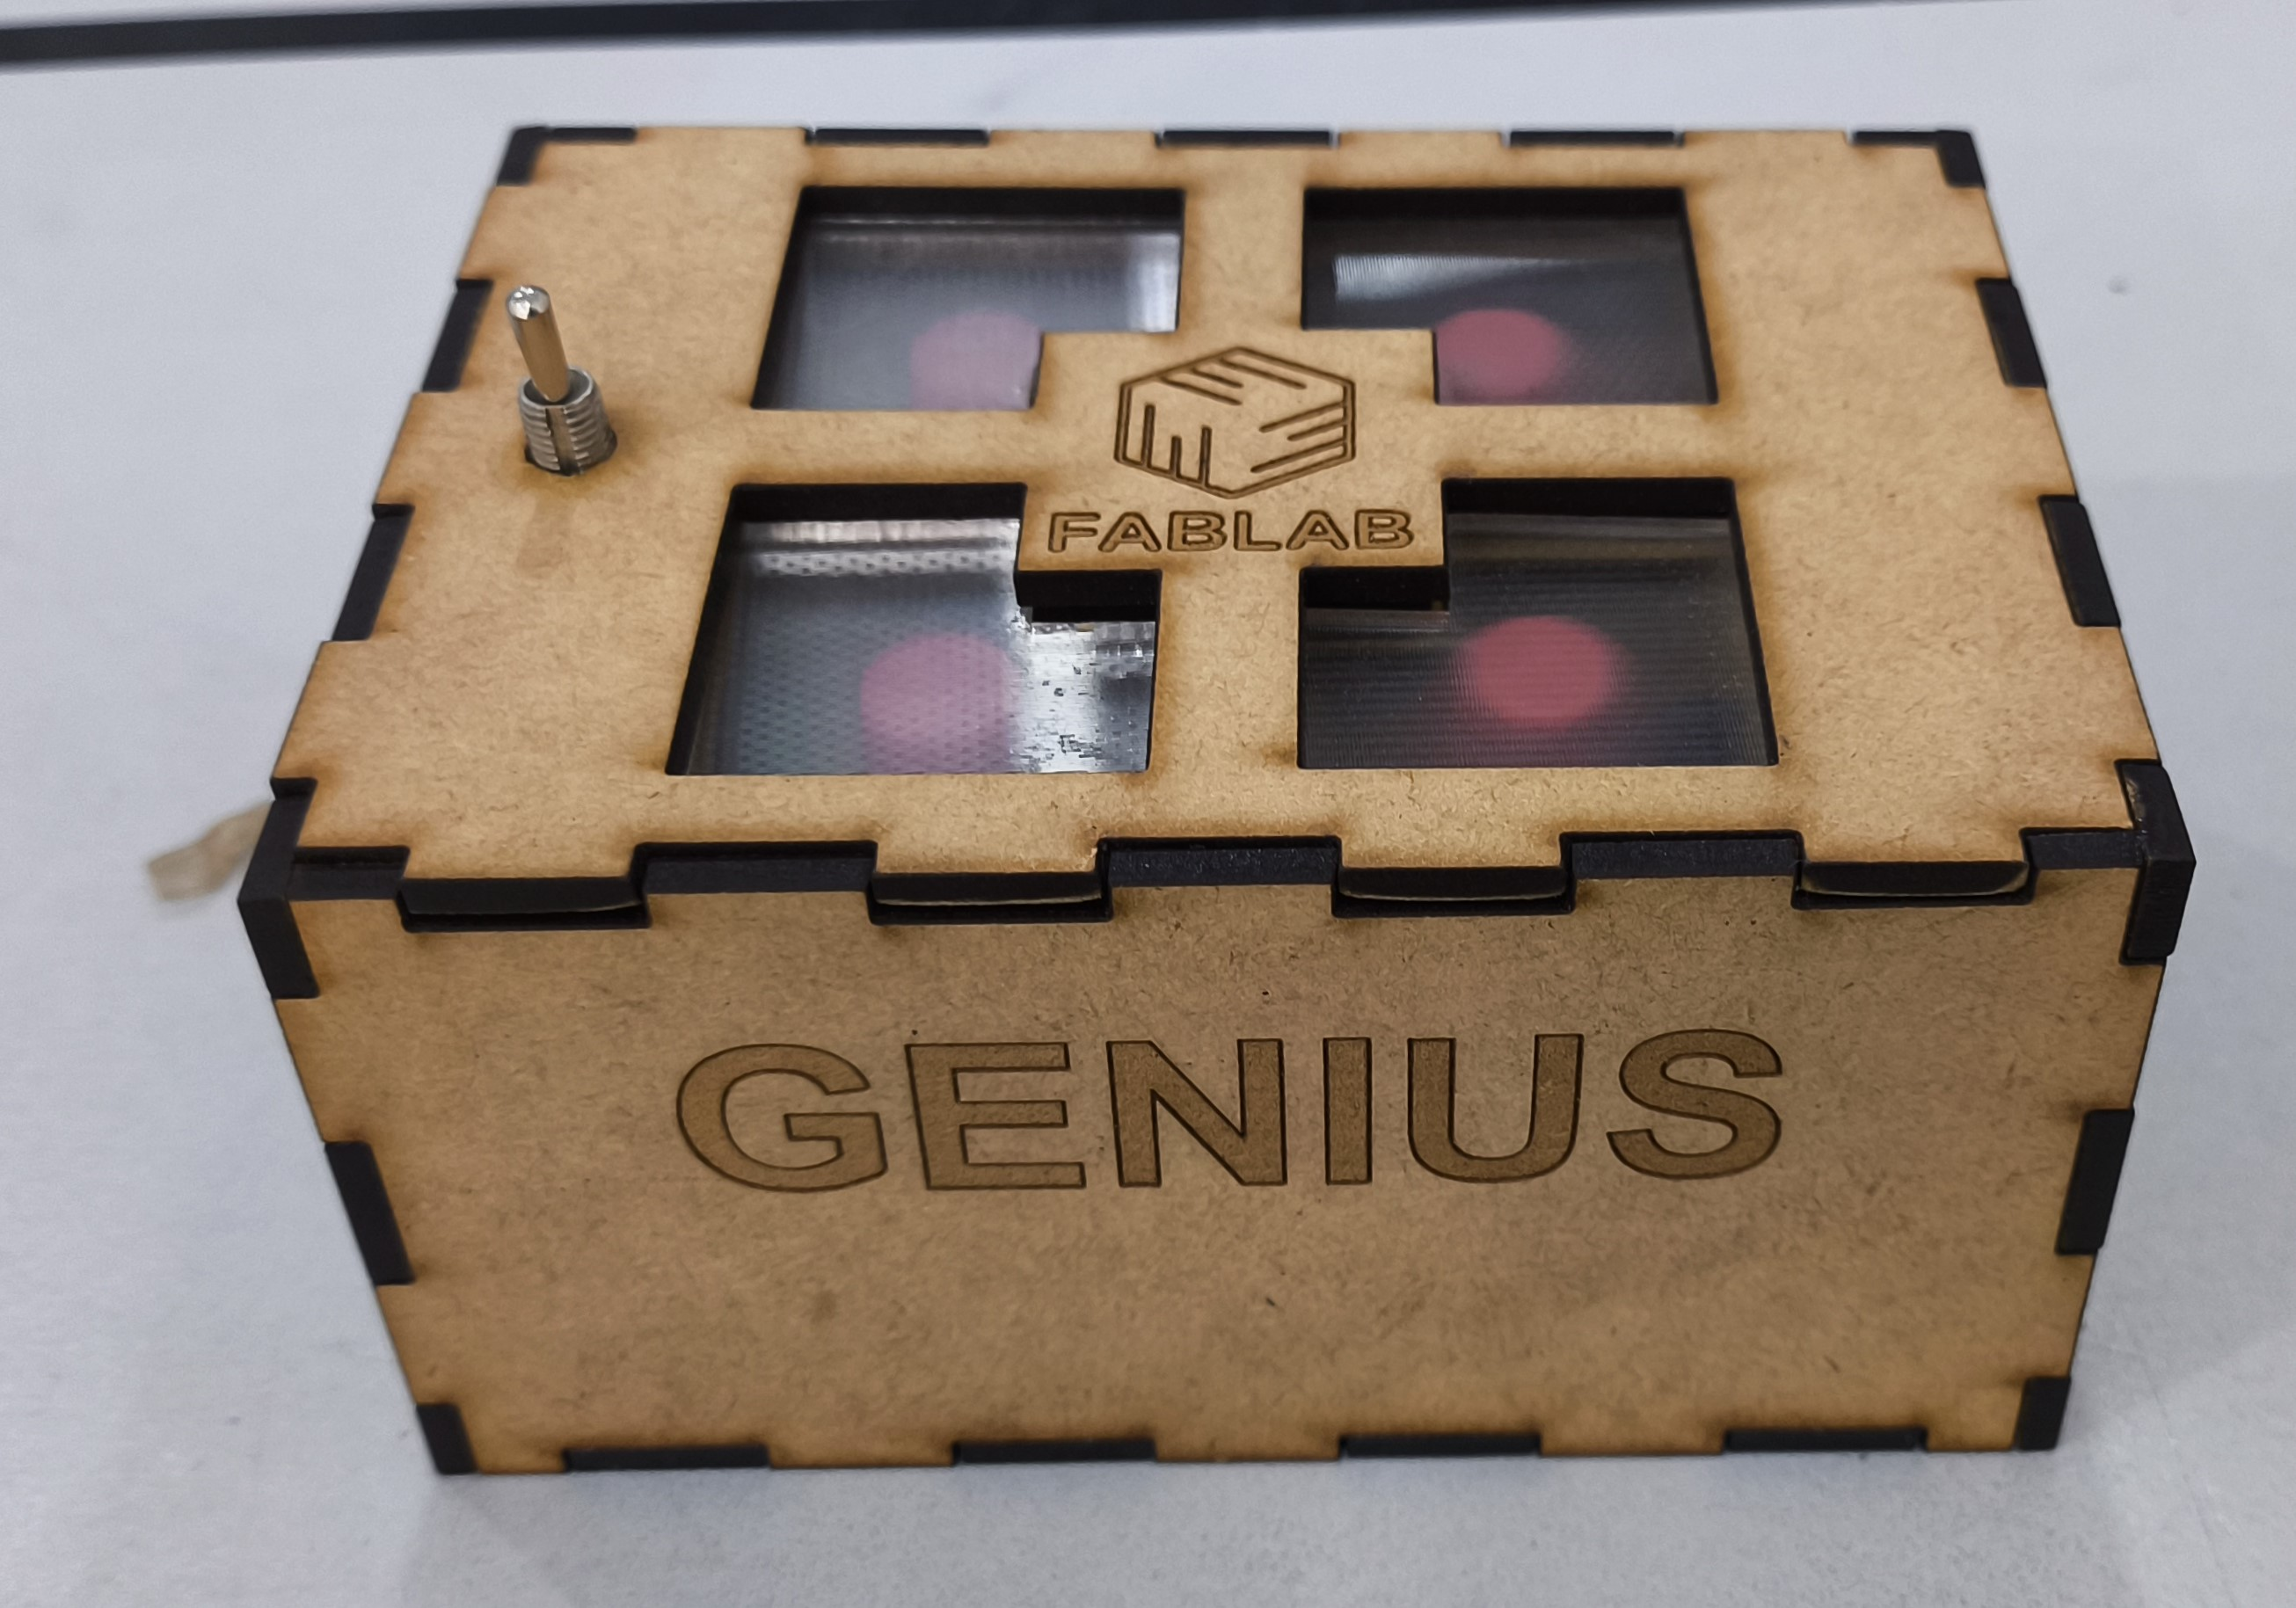
\includegraphics[width=0.5\textwidth,height=\textheight]{D:/Minha pasta/Estudos/UFPA/8º Semestre - 2024.2/Tópico Especiais em Eletrônica/Aluno/Ryan TEE/38.jpg}

Fig 39: Vista frontal da caixa.

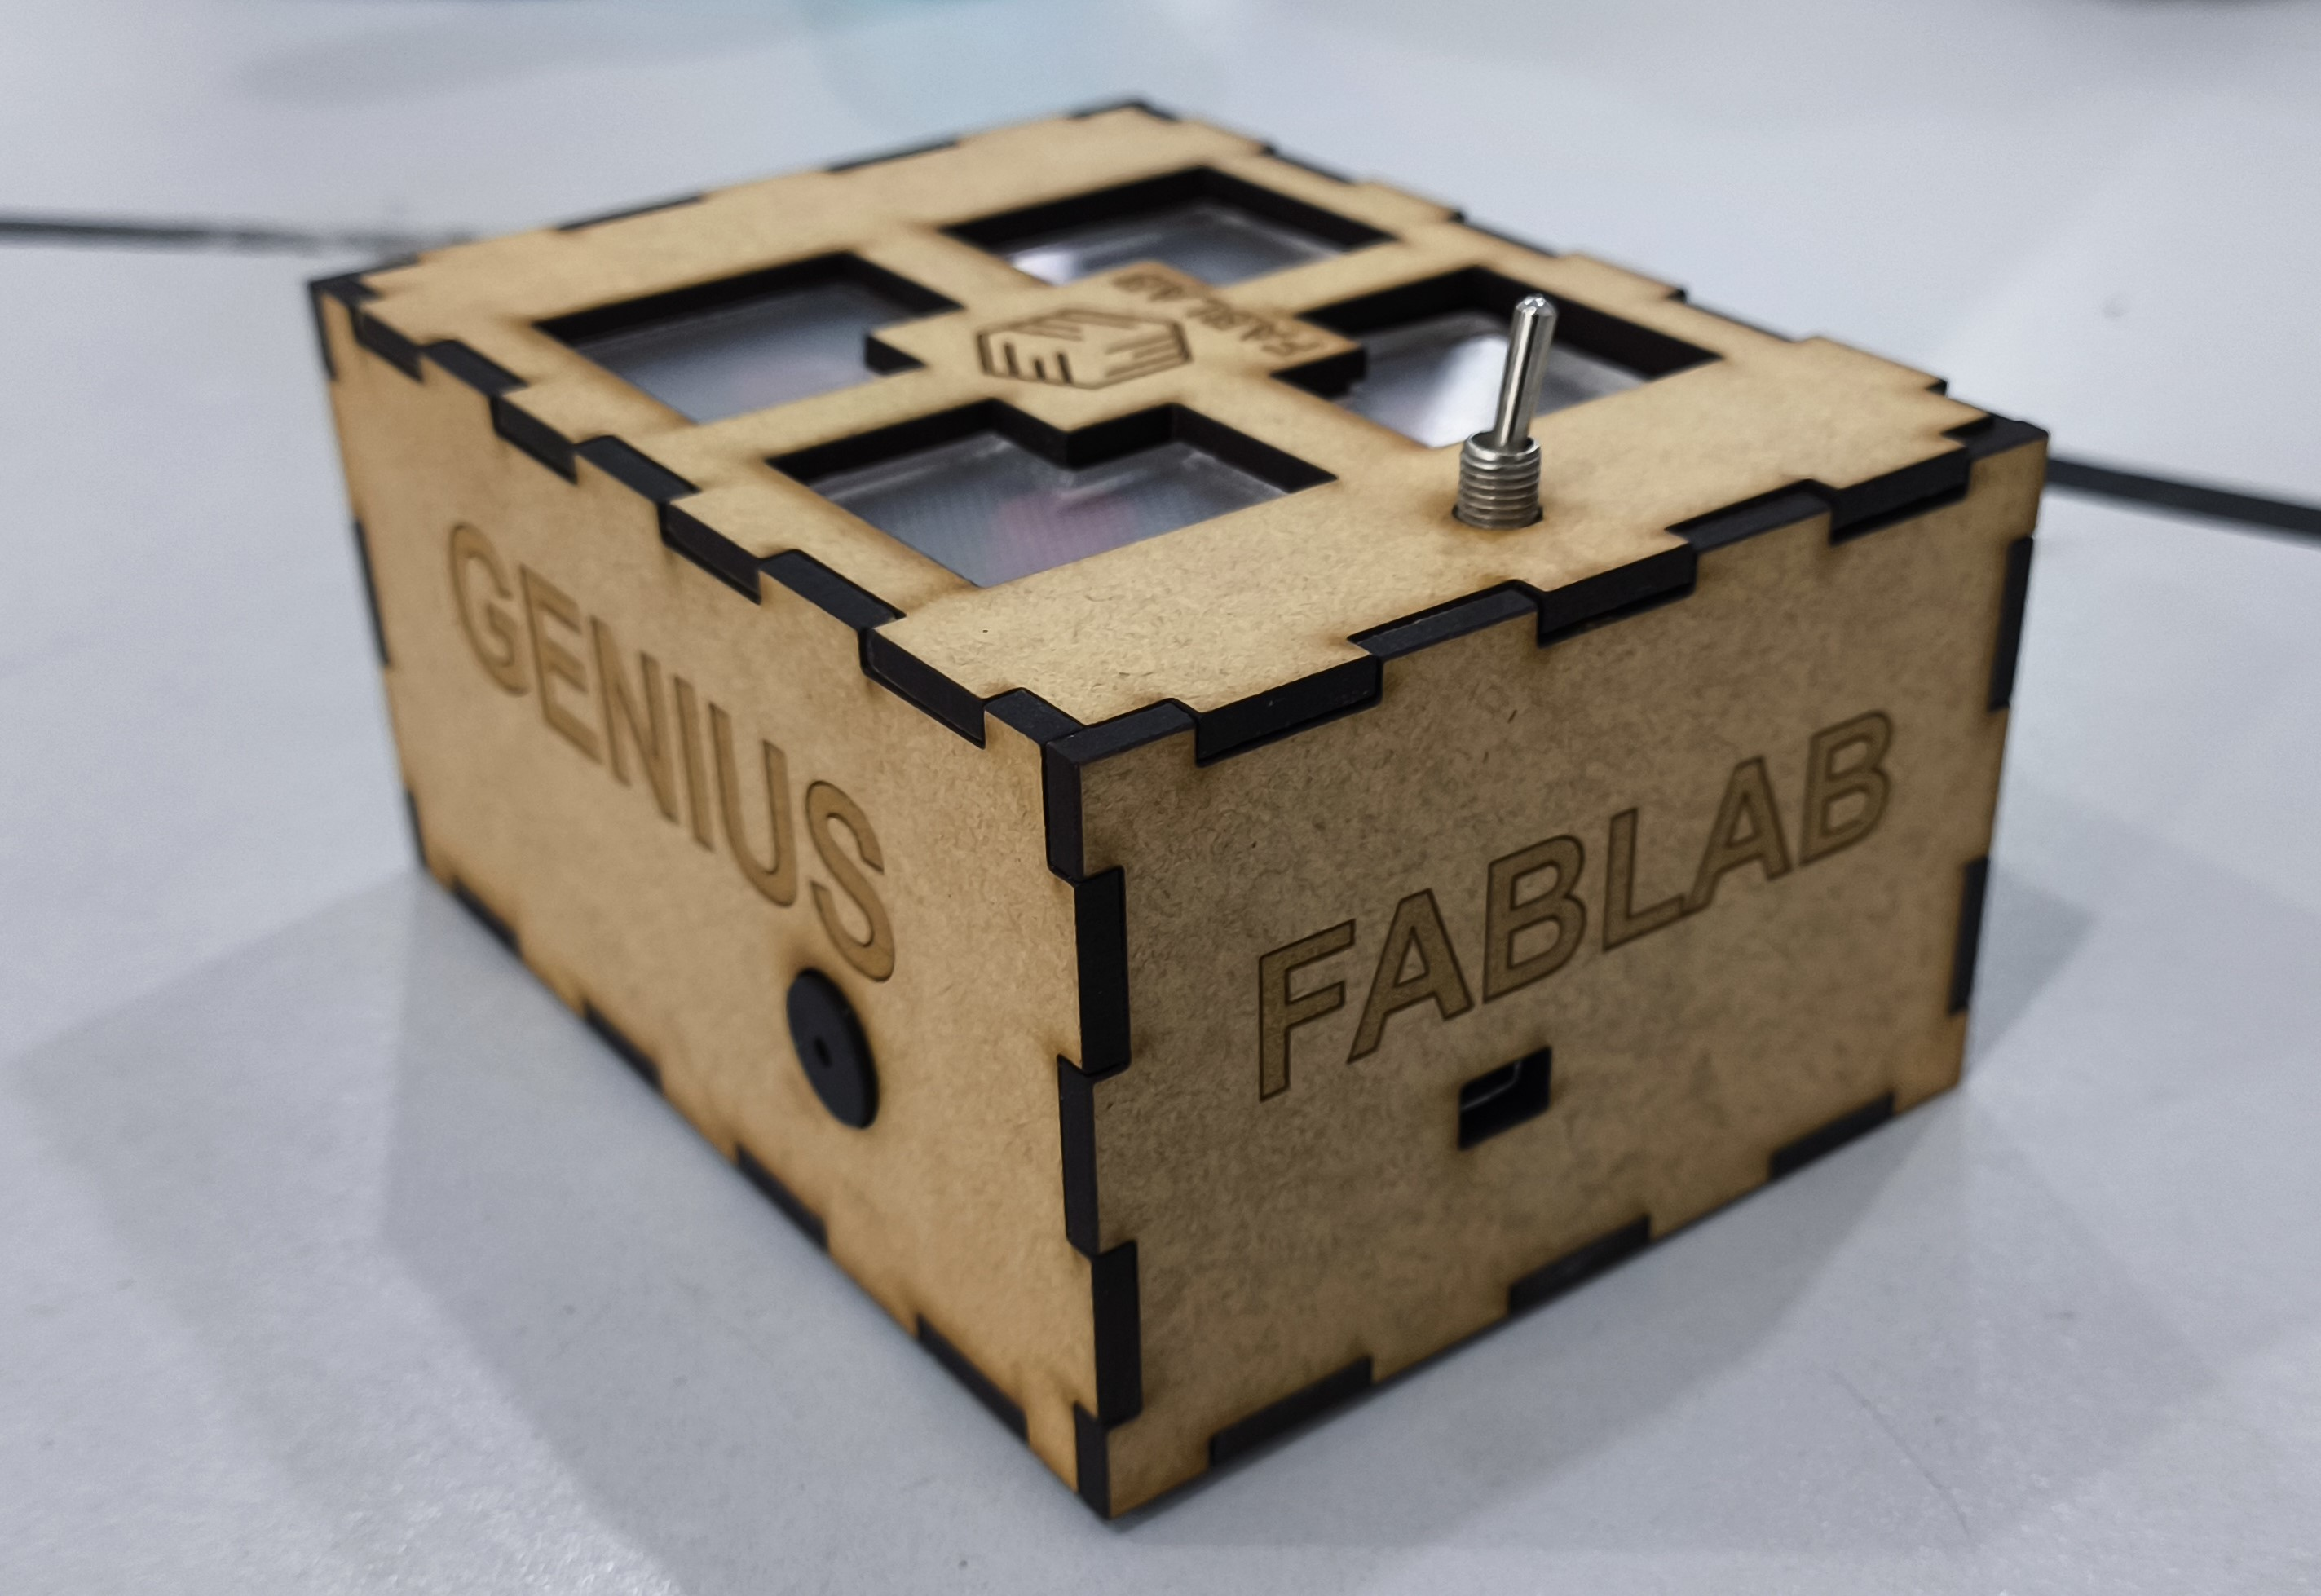
\includegraphics[width=0.5\textwidth,height=\textheight]{D:/Minha pasta/Estudos/UFPA/8º Semestre - 2024.2/Tópico Especiais em Eletrônica/Aluno/Ryan TEE/39.jpg}

Fig 40: Vista lateral da caixa.

Como monitor da disciplina, também participei ativamente no desenvolvimento dos projetos dos meus colegas. Isso incluiu auxiliar na criação de circuitos impressos, orientar na produção de peças utilizando impressoras 3D e o laser, oferecer suporte na parte mecânica dos projetos e ajudar com o código, além de prestar outras formas de assistência necessárias.

\chapter{CONCLUSÃO}\label{conclusuxe3o}

A disciplina como um todo foi extremamente proveitosa, proporcionando aos alunos conhecimentos práticos sobre máquinas e ferramentas que são muito úteis na vida acadêmica e profissional. Ela permitiu sair um pouco do meio tradicional de ensino universitário, oferecendo uma experiência mais prática.

O projeto final foi uma oportunidade única para os alunos aplicarem os conhecimentos adquiridos ao longo da disciplina e do curso como um todo. Essa prática é fundamental para estudantes prestes a se formarem, pois permite idealizar um projeto, colocá-lo em prática e vivenciar todo o processo, incluindo as dificuldades e os erros que surgem ao longo do caminho. A capacidade de resolver problemas e fazer ajustes é um conhecimento valioso que nem sempre é ensinado de maneira tradicional em sala de aula. Essa experiência é extremamente enriquecedora para os futuros engenheiros, independentemente da área de atuação que escolham seguir.

  \bibliography{book.bib,packages.bib}

\end{document}
